\documentclass[11pt]{article}
\usepackage[T1]{fontenc}
\usepackage[utf8]{inputenc}
\usepackage{lmodern}
\usepackage[margin=1in]{geometry}
\usepackage{amsmath,amssymb}
\usepackage{graphicx}
\usepackage{booktabs}
\usepackage{array}
\usepackage{tabularx}
\usepackage{multirow}
\usepackage{longtable}
\usepackage{placeins}
\usepackage{xcolor}
\usepackage[numbers,sort&compress]{natbib}
\usepackage{microtype}
\usepackage[colorlinks=true,linkcolor=blue!50!black,citecolor=blue!50!black,urlcolor=blue!50!black]{hyperref}

\usepackage{etoolbox}\makeatletter\patchcmd{\l@section}{1.5em}{2.0em}{}{}\makeatother% room for S10 in the contents
\newcommand{\gap}{\mathrm{gap}}
\newcommand{\tbd}[1]{\textcolor{red}{[#1]}}
\newcommand{\BT}{Base$\leftrightarrow$Turbo}
\newcommand{\TT}{ZIT-25}% the 25-step, CFG 4, pooled Z-Image Turbo campaign (its archive files are labelled "ZIB"/Z-Image Base)
\newcolumntype{L}{>{\raggedright\arraybackslash}X}
\graphicspath{{figures/}}

\title{What Recurs and What Is Shared:\\
Layerwise Spectral Telemetry of Generative Transformers\\[4pt]
\large Mode-I: an empirical atlas and its falsification record\\[2pt]}
\author{Zac Doyle\\ \small mode:LIMINAL\\ \small ORCID \href{https://orcid.org/0009-0006-0452-1374}{0009-0006-0452-1374}\\ \small \url{https://github.com/Z-L-D/mode-I}}
\date{November 2026\\ \small Version of 11 November 2026}

\begin{document}
\maketitle

\begin{abstract}
Comparing generative models by their internal dynamics needs an observable that follows the model rather than the capture. We record three spectral statistics of the token activation matrix (a normalised participation ratio $g$, the leading singular-value gap and the spectral entropy $H$) at every layer and sampling step of diffusion and flow transformers for images, video and audio, each at its recommended operating point, over 18 audit rounds, 17 of them with hashed preregistration. Scalar envelopes cannot compare models: their ordering of model pairs follows the capture, and an unrelated pair can outscore the same weights.

The positive result is conditional and narrow. The attention depth tangent, a cosine between depth differences of standardised layer profiles, places every related pair we measured at equal depth above its nulls and every measured unrelated pair at or inside them. It is a screen, not a detector: with no false positive among two unrelated pair types (five model pairs), the one-sided 95\% upper bound on its false-positive rate is $78\%$ ($45\%$), and the related pairs share more architecture than the unrelated ones, so the split may reflect architecture as well as training relation. Until an architecture control is run, the split is between the model families measured, not between training relations in general, and at these bounds the screen cannot serve as a decision rule where a false positive is costly. We read it on a native grid with one point per hooked layer, chosen after the preregistered 24-point analysis so that interpolation averages no layer away, and report the 24-point values beside it. Same-weights controls, a distillation family, a same-vendor successor and a sibling pair (Z-Image Base and Turbo, derived separately within one family) lie above their nulls; two kinds of unrelated pair lie at or inside them ($-0.17$ to $0.20$). The split holds on the native, 24- and 48-point grids and on the middle third of depth, not on a 12-point grid, because the lowest depth frequencies agree across unrelated pairs too and the separating signal sits in depth structure a few layers long (post hoc); the tangent is not calibrated across depth; in MLP it does not separate an unrelated pair ($0.57$; $0.69$ on 24 points), whose agreement sits in the slowest depth trends and the shared mean direction (centred, $0.27$; post hoc); and about 60 independent unrelated pairs would be needed to bound the false-positive rate at $5\%$. Within the related pairs we read an ordering hypothesis of three tiers, same weights ($0.98$--$1.00$; $0.92$ for one model across capture sessions) above the successor ($0.93$) and a documented teacher--student pair (SD3.5 Large and Large Turbo, $0.90$; its preregistered rule returns the middle tier, $0.82$ on 24 points) above the other distillation pairs ($0.80$--$0.85$), as informed speculation to be revisited. The Z-Image siblings show that separately derived models of one family still share a measurable depth dynamics, but whether they pass the lineage rule depends on the grid and where they sit depends on the rows read: $0.55$ on all rows, above both nulls by $0.26$ and short of the $0.30$ lineage rule ($0.71$ on the 24-point grid), and $0.91$ on image rows, level with the successor. The sibling value does not depend on Base's sampling shift ($0.52$ at the official shift $6$). A preregistered but coarse activation baseline (linear CKA on 36-token float16 sketches of nine models) ranks related above unrelated pairs well (rank AUC $0.97$) but does not separate them: the siblings fall below two of the 21 unrelated pairs, all of which also exceed its null, and it does not reproduce the tangent's ordering. Every statistic is of the uncentred second moment; which results survive centring or image rows is marked where they are stated.

A first-state identity check caught a mislabelled campaign but does not separate close relatives. A weak but reliable component of prompt-relational geometry is shared across unrelated image and video models. Refuted predictions are reported with equal weight, practical capture rules are given, and preregistrations, audit trail and code are released.
\end{abstract}

\begin{center}
\fbox{\begin{minipage}{0.94\linewidth}\small
\textbf{Main results at a glance.}
\begin{itemize}\setlength\itemsep{1pt}
 \item \emph{Observable hierarchy.} Scalar envelopes cannot tell a model from an unrelated one. \emph{Measured:} among the depth-matched pairs measured (six related pairs from four families plus same-weights controls; two unrelated pair types), the related pairs sit above their attention-tangent nulls and the unrelated pairs at or inside them ($-0.17$ to $0.20$ on the native grid, one point per hooked layer; up to $0.30$ on the preregistered 24-point grid), on native, 24- and 48-point grids and on the middle third of depth, not on a 12-point grid; the screen's false-positive rate is not established (\S\ref{sec:tierstatus}). \emph{Working hypothesis:} three tiers within that split, same weights ($0.98$--$1.00$ in a session; $0.92$--$1.00$ across sessions, attention), a same-vendor successor ($0.93$), distillation pairs ($0.80$--$0.90$, the upper value a documented teacher--student pair, Round 18); the boundary between the upper two is not established (\S\ref{sec:tierstatus}). A preregistered activation-CKA baseline on nine of the models does not separate related from unrelated pairs (\S\ref{sec:cka}). The Z-Image sibling pair, related through an unreleased model, sits between distillation and unrelated pairs on all rows ($0.55$; $0.71$ on 24 points) and level with the successor on image rows ($0.91$). The MLP tangent does not separate an unrelated pair ($0.57$; $0.69$ on 24 points). Cross-depth tangents are not calibrated (\S\ref{sec:depthcal}).
 \item \emph{Audit.} A first-state identity check separates Base from distilled checkpoints from one generation and caught an archive campaign whose label did not match its weights. Over all 66 different-checkpoint pairs of equal depth no value reaches $0.95$, but it reads SD3 and SD3.5 Medium as close ($0.93$--$0.94$); it is an audit heuristic, not a calibrated classifier, and a weight hash supersedes it where one is recorded.
 \item \emph{Content.} Prompt-relational geometry is shared across unrelated models, beyond wording and length, and on image-only and centred rows; it does not tier by lineage.
 \item \emph{Sampling.} Prompt geometry reaches the unconditional branch in the first 10\% of steps; distilled checkpoints are less seed-sensitive than their Base models (post hoc).
 \item \emph{Scope.} The $+,-,+,-$ depth sequence and the Z-Image MLP clock-axis contraction are properties of particular models and capture settings; Z-Image MLP statistics are caption-row statistics (Table~\ref{tab:captionmap}).
 \item \emph{Estimators.} A pooling theorem (Mode-II) fixes the sign of the capture-functional bias; the raw $\sigma_{50}$ onset is a sample-size number and is replaced.
 \item \emph{Practical use.} Never compare $g$ across capture functionals; capture the conditional branch, image rows and the weight hash; run the identity gate on every capture; read the tangent on depth-matched attention only (\S\ref{sec:practice}).
\end{itemize}
\end{minipage}}
\end{center}

\begin{table}[p]
\centering\scriptsize
\caption{Primary claims, the strength of their evidence and their scope. Evidence: OOS, preregistered before the data existed (out of sample); PA, preregistered before scoring, on archive data explored in earlier rounds; LA, preregistered with thresholds set with related data in view (lookahead, disclosed in \S\ref{sec:instrument}); KV, preregistered nulls or resampling added to values already known; PH, post hoc, a hypothesis unless replicated; R, review reproduction, not preregistered. $p$: permutation $p$ of the test named (at its resolution floor where so marked); BH $q$: Benjamini--Hochberg over the seven $p$-values in this table (descriptive). Rules without a $p$-value are threshold criteria. The tangent screen's false-positive rate is not established: a $5\%$ bound needs about 60 independent depth-matched unrelated pairs; there are two pair types (\S\ref{sec:tierstatus}).}
\label{tab:primary}
\renewcommand{\arraystretch}{0.82}\setlength\tabcolsep{4pt}\begin{tabularx}{\linewidth}{@{}>{\raggedright\arraybackslash}p{3.2cm}>{\raggedright\arraybackslash}p{1.8cm}>{\raggedright\arraybackslash}p{1.5cm}c>{\raggedright\arraybackslash}X@{}}
\toprule
Claim & Evidence & Round & $p$ (BH $q$) & Scope\\
\midrule
Low-dimensional depth--time backbone & R; OOS replication & 1; 11 & $0.001^{\dagger}$ ($0.0012$) & every transformer channel; U-Net, ACE-Step post hoc\\
Related above unrelated (attention tangent) & LA; OOS; PH (grid) & 12, 14, 16--18; RC26 & $0.0001^{\ddagger}$ ($0.0004$) & depth-matched; 8 related and 2 unrelated pair types; holds on the native grid and at 24 and 48 points, not at 12\\
Sibling pair, Z-Image & LA; KV (R15); PH (native) & 12; 15; RC33 & $0.0001^{\ddagger}$ ($0.0004$) & native grid $0.55$ attention, $0.26$ above both nulls, short of the $0.30$ rule ($p=0.0003$, 10{,}000 draws); prereg.\ 24-point value $0.71$; on image rows attention ($0.928$) fails the $0.10$ margin and sits $0.014$ below the pooled same-weights value\\
Lineage tier, ACE-Step & OOS & 14, 16 & $0.0003^{\ddagger}$ ($0.0005$) & holds at 6 and 8 steps; MLP from the last layers; attention $0.25$--$0.27$ above the surrogate p95\\
Three tiers within related pairs & hypothesis & 12--18 & -- & six pairs; same weights vs successor not separated ($0.92$ vs $0.93$); documented distillation level with the successor\\
Middle tier without distillation & OOS (rule) & 17 & -- & SD3 M$\leftrightarrow$SD3.5 M $0.93$, attention\\
Documented distillation in the middle tier & OOS (rule) & 18 & -- & SD3.5 L$\leftrightarrow$L Turbo $0.818$ on 24 points ($0.904$ native), attention\\
This coarse CKA baseline does not separate related from unrelated pairs & OOS (rules) & 18 (B) & -- & related above chance (B1), but not separated from unrelated (B2, AUC $0.968$) and not in the tangent's order (B3, $0.70$); 36-token float16 sketches\\
Unrelated pairs at or near null & PH; OOS & RC5; 17 & -- & attention only: $-0.17$ to $0.20$ native, $0.30$ on 24 points; MLP refuted ($0.57$ native, $0.69$)\\
Identity check separates checkpoints & PH & RC10, RC27 & -- & equal depth; 0 of 66 different pairs $\ge0.95$; not SD3 vs SD3.5 M ($0.94$)\\
A related-looking unrelated value in MLP & R & 15 & -- & Qwen3.5-0.8B$\leftrightarrow$Qwen2.5-1.5B MLP $0.66$ (null $0.32$); with PixArt--Cosmos MLP, why MLP is not tiered\\
Shared prompt geometry & PA & 6, 8 & $\le0.0002^{\ddagger}$ ($0.0005$) & weak but reliable ($\rho=0.13$--$0.43$ unrelated); at default operating points; beyond text and length\\
First-state domain decoding & R & 1 & $0.01^{\dagger}$ ($0.01$) & visual-stream channels\\
Text-to-latent handoff & OOS & 15 & -- & 4 of 5 channels\\
Z-Image Turbo MLP clock contraction & PA & 6 (S4) & $\le0.001^{\dagger}$ ($0.0012$) & Turbo caption rows; absent in Base\\
Caption rows carry Z-Image MLP energy & OOS (R11-7 refuted) & 11 & -- & from layer 10 on\\
Relative onset replaces $\sigma_{50}$ & PA & 6 (S3) & -- & 7 of 7 channels\\
Distilled students less seed-sensitive & PH & -- & bootstrap & two families; guidance-confounded\\
$+,-,+,-$ layer sequence & PA, descriptive & 6 & see Table~\ref{tab:beta} & per channel with surrogate class\\
\bottomrule
\end{tabularx}
\par\smallskip\raggedright\scriptsize $^{\dagger}$ at the resolution floor of the test as run (1{,}000 draws; 100 for domain decoding). $^{\ddagger}$ re-run with 10{,}000 permutations (post hoc, RC30 for the tangent rows: no draw of any related pair reaches its value except ACE-Step MLP, 1--2 draws; RC32 for the prompt Mantel tests: every unrelated cell $p\le0.0002$); $p=(k+1)/(N+1)$, so $0.0001$ is again a floor; tangent rows give the largest $p$ over their pairs and submodules. Under a global null the expected number of these seven $p$-values at or below their observed values is their sum, $0.0127$ (linearity of expectation; no independence needed; not itself a $p$-value). The tests share captures, so BH, valid under the positive dependence this plausibly induces, is descriptive, and $q$ inherits each floor; every $q\le0.01$. Under a Bonferroni correction at $0.05/7=0.0071$ the six claims at $p\le0.001$ survive and first-state domain decoding ($p=0.01$) does not. Labels: end of \S\ref{sec:intro}.
\end{table}

{\small\tableofcontents}
\newpage

%=====================================================================
%=====================================================================
\section{Introduction}\label{sec:intro}

Comparisons between generative models usually look at their outputs or at static representations of fixed inputs \citep{raghu2017svcca,kornblith2019similarity}. A diffusion or flow transformer, however, computes a trajectory: at each sampling step the network transforms its input through a stack of layers, and the sampler then moves the latent to a lower noise level \citep{ho2020denoising,song2021scorebased,lipman2023flow,liu2023flow}. The object we study is the evolution of layerwise spectral geometry along both axes of that computation, depth and sampling time.

We use a fixed passive instrument (the CoS-PAFS capture node, from the Chain-of-Steps Phase-Adaptive Flow Solver project) that records, for every layer, step and generation, three statistics of the token activation matrix: the normalised amplitude participation ratio $g$, the spectral gap and the spectral entropy. The archive holds four diffusion and flow transformers captured on a common set of prompts, with Z-Image Turbo captured twice, at its native 8 steps without guidance (ZIT) and at 25 steps with guidance and pooled capture (\TT{}; its archive files are labelled Z-Image Base, but the identity gate of \S\ref{sec:similarity} shows it is Turbo). The real Z-Image Base was captured separately (Rounds 11--12). Turbo is a few-step model distilled within the Z-Image family: the technical report describes few-step distillation of ``our foundational SFT model'' with Decoupled DMD and DMDR, and labels the distilled result Z-Image-Turbo (\citealp[\S4.5 and Fig.~13]{zimageteam2025zimage}; \citealp{liu2025decoupled}). Base is the released undistilled model of the same family \citep{tongyi2026zimage}; the report does not name it, and does not say whether it is the SFT model's initialisation. Base is therefore most likely a sibling of Turbo's teacher, not the teacher itself. We call a Base model and its distilled checkpoint a \emph{lineage pair}, and what such a pair has in common beyond unrelated models \emph{shared within a lineage}; the word names the relation, not the mechanism, and ``family'' would be an equally fair name. The design cannot separate what the distillation objective transmitted from what the two models already shared through common pretraining, data and text encoder. There are two lineage pairs: Z-Image Base and Turbo, and ACE-Step~1.5 Base and its distilled turbo checkpoint. For ACE-Step the release describes turbo as the distilled version of the model; which checkpoint served as its teacher is not documented in the material we used. Both students are also few-step models, so in Z-Image step count and distillation are not separated (in ACE-Step the Base arm separates them for the depth sign sequence, \S\ref{sec:ace}). The other pairs are unrelated architectures, a scaling pair, or the same weights under changed inference. Two further models were captured as out-of-family checks: the convolutional U-Net of Stable Diffusion~1.5 (\S\ref{sec:unet}) and the audio flow transformer ACE-Step~1.5, in both checkpoints (\S\ref{sec:ace}).

We ask empirical questions and do not assume a universal answer:
\begin{enumerate}
 \item Is the measured trajectory low-dimensional, and is that more than smoothness?
 \item Do trajectories of unrelated models resemble each other, and at which level of description?
 \item Does depth geometry carry information about prompt content, and is the content geometry shared across models?
 \item Is there a recurrent sign structure along the sampling clock or along depth, and does it survive null models?
 \item What can passive telemetry say about when a seed's outcome becomes predictable?
 \item Which interventions (guidance, ablation, scale, distillation) preserve which geometry?
\end{enumerate}

\paragraph{Release boundary.} This paper makes no claim about a separatrix or commitment boundary in the sampling dynamics, about any relation between the geometry and output quality, about per-token phases in autoregressive models, or about a renormalisation-group universality class. The data cannot support these claims, and Section~\ref{sec:limits} lists the experiments that could.

\paragraph{Contributions.}
\begin{enumerate}
 \item A multi-model telemetry atlas with named capture regimes and a released reproducer for every number (\S\ref{sec:instrument}).
 \item Low-dimensional depth--time organisation of the measured geometry, beyond smoothness (\S\ref{sec:backbone}).
 \item An observable hierarchy: scalar resemblance crosses architecture boundaries, while attention depth tangents separate related from unrelated depth-matched model pairs and suggest, as a hypothesis to be revisited, a finer ordering (same weights and a same-vendor successor above a Base--distilled pair and a sibling pair, ordered on the native grid), and MLP tangents do not; stated cell by cell, and the tangent's dependence on depth and on each coordinate is characterised (\S\ref{sec:similarity}).
 \item Semantic information in ordered depth geometry and broadly shared prompt-relational geometry (\S\ref{sec:content}).
 \item Two separately scoped sign-structure results, along the sampling clock and along depth, with bootstrap and surrogate qualification (\S\ref{sec:topology}).
 \item Calibrated estimators for seed predictability that remove a sample-size artefact (\S\ref{sec:seed}), an intervention hierarchy (\S\ref{sec:interventions}), and a falsification record that defines the claim boundary (\S\ref{sec:falsification}).
 \item Preregistered out-of-family checks on a convolutional U-Net (\S\ref{sec:unet}) and on an audio flow transformer in its distilled and undistilled checkpoints (\S\ref{sec:ace}), which separate the results that hold outside the image-transformer setting from those that do not.
 \item A model-identity check from first-state depth profiles, an audit heuristic with its behaviour on every labelled pair of equal depth, which separates Base from distilled checkpoints but not SD3 from SD3.5 Medium, and caught an archive campaign whose label did not match its weights (\S\ref{sec:gate}).
\end{enumerate}
The mathematical treatment of these results (a pooling theorem, projection degeneracy, the non-autonomous flow family and null derivations) is given in the companion paper, Mode-II. The split follows the two kinds of claim: this paper's claims are empirical, scoped to captures and falsifiable by new captures, while Mode-II's are proofs and null constructions that hold whatever the data. Each paper states the results it imports from the other with their status (Appendix~\ref{app:imports} here). One of Mode-II's results frames how every comparison below should be read: the triple is invariant to every orthogonal change of basis of the residual stream under RMSNorm, and to signed channel permutations under adaptive normalisation (Mode-II, Lemma~9 and Corollary~10), so agreement in these coordinates is necessary for a functional correspondence between two models but never sufficient. Language-model telemetry with context-invariant statistics, and the relation between a diffusion model and its text encoder, are the subject of the next paper in the series, Mode-III.

\paragraph{Reader's guide.} Table~\ref{tab:primary} lists the primary claims with their status. The core results are in \S\ref{sec:similarity} (the tiers, their depth calibration and the identity gate) and \S\ref{sec:content}; \S\ref{sec:topology}--\S\ref{sec:interventions} are scoped descriptive results, and \S\ref{sec:falsification} records what did not survive. Table~\ref{tab:retired} lists the retired claims. The appendices hold capture provenance (\ref{app:provenance}), the preregistration scorecards (\ref{app:prereg}) and the results imported from Mode-II (\ref{app:imports}); the labels used throughout are decoded in the label list at the end of this section. Detail that supports but does not carry a claim is in the Supplementary material after the appendices, with a pointer at each place it is used: tangent robustness (\ref{supp:tangent}), the identity-gate table (\ref{supp:gate}), layer-axis surrogates and per-step nulls (\ref{supp:beta}), the falsification record in full (\ref{supp:fals}), analyzer notes (\ref{app:analyzer}), estimator sensitivity (\ref{app:estimators}), legacy-instrument results (\ref{app:legacy}), capture cost (\ref{supp:cost}) and supplementary figures (\ref{app:supp}). Six practical rules are collected in \S\ref{sec:practice}. The labels used most often are: ZIT, Z-Image Turbo at its native 8 steps; \TT{}, Turbo at 25 steps with guidance, pooled (archive files labelled ZIB); Z1 and Z2, real Z-Image Base at CFG 4 and 1; Z3, Turbo at Base's settings; ACEB and ACET, ACE-Step Base and turbo; T8 and T$k$, turbo at 8 and $k$ steps; R$n$-$k$, prediction $k$ of Round $n$; RC$k$, review check $k$. Appendix~\ref{app:glossary} has the full list.

\paragraph{Labels and terms.}\label{sec:labels} The labels used throughout are decoded here. Three examples show how to read them. ``R18-1 (OOS)'' is prediction 1 of Round 18, frozen before its capture existed and scored once. ``RC33 (post hoc)'' is review check 33, run on existing captures after the values were known, so its results are hypotheses. ``Z1$\leftrightarrow$ZIT, native, $0.547$'' is the tangent between the real Base capture Z1 and Turbo at 8 steps, read on the native grid; the same pair on the preregistered 24-point grid is $0.707$.

{\small\noindent
\begin{tabularx}{\linewidth}{@{}lL@{}}
\toprule
Term & Meaning\\
\midrule
ZIT & Z-Image Turbo at its native 8 steps, CFG 1, cond-only (archive)\\
\TT{} & Z-Image Turbo at 25 steps, CFG 4, pooled capture (archive files labelled ZIB / Z-Image Base)\\
Z1, Z1U & real Z-Image Base, 25 steps, CFG 4, conditional / unconditional branch (Round 12)\\
Z2 & real Z-Image Base, CFG 1, cond-only, with row-split variants (Rounds 11 and 12)\\
Z3 & Z-Image Turbo at the Z1 settings (Round 12)\\
ACEB, ACET & ACE-Step 1.5 Base (Round 14; 50 steps, CFG 4) and turbo (Round 3; 6 steps, shift 3, no CFG) checkpoints\\
T8, T$k$ & ACE-Step turbo recaptured on the Base prompts and seeds at 8 steps and at $k$ steps (Round 16)\\
Round 17 arms & PixArt-$\Sigma$ XL (20 steps, CFG 4.5), Cosmos-Predict2 2B (35 steps, CFG 7), SD3 Medium (28 steps, CFG 7), SD3.5 Medium (40 steps, CFG 4.5); 60 prompts, seed 1001\\
Same weights & two captures of one checkpoint under changed inference or capture\\
Lineage pair & two related checkpoints: \emph{distillation lineage}, a Base model and its distilled student (Z-Image, ACE-Step); \emph{successor lineage}, a later model of one vendor and line whose training relation is not documented (SD3 Medium$\leftrightarrow$SD3.5 Medium); \emph{sibling lineage}, two models derived separately within one family, neither from the other (Z-Image Base and Turbo, whose teacher is an unreleased SFT model). The word names the relation, not the mechanism\\
Capture functional & pooled, cond-only or branch-mean recording of a CFG step (\S\ref{sec:instrument})\\
Tangent & matched-$\sigma$ cosine of depth differences of standardised profiles on the native grid (one point per hooked layer of the shallower model) or the preregistered 24-point grid (Mode-II, Def.~8)\\Native grid & a depth grid with as many points as the shallower model of a pair has hooked layers (24, 28 or 30 here); no layer is averaged away by interpolation\\
Shape & correlation of standardised, registered depth profiles\\
Identity gate & step-0 depth-profile correlation with a reference checkpoint (\S\ref{sec:gate})\\
$\beta_{\rm layer}$ & layer step $g_{\ell+1}-g_\ell$ (analyzer's layer-direction flow)\\
Relative onset & $\sigma$ at which seed predictability reaches half its own ceiling (\S\ref{sec:seed})\\
R$n$-$k$, S$k$, B$k$, C$k$ & preregistered prediction $k$ of Round $n$; Round 6 S-tests; ACE-Step (B) and U-Net (C) predictions\\
G1--G4 & standing gates for claims not made here (\S\ref{sec:instrument}, \S\ref{sec:limits})\\
RC$k$ & post hoc review check $k$ (\texttt{review/r15\_deep\_dive/review\_checks/}); not a prediction, unlike R$n$-$k$\\
D$k$, ledger card & a numbered entry of the project's internal findings ledger, with its reproducer (Mode-II cites them; the ledger is available on request)\\
Register & the release claim register, the internal list of claims with status and source fixed for the release (available on request)\\
Lineage cell & one (family, submodule) combination of a lineage pair: Z-Image or ACE-Step, attention or MLP\\
CoS-PAFS & Chain-of-Steps Phase-Adaptive Flow Solver, the project whose capture node and analyzer are used here\\
\bottomrule
\end{tabularx}
}

%=====================================================================
\section{Related work}\label{sec:related}

\paragraph{Representation geometry along depth.} Linear and nonlinear dimension estimates of hidden representations change systematically with depth \citep{ansuini2019intrinsic,recanatesi2019dimensionality}, and their coarse depth profiles recur across very different transformers \citep{valeriani2023geometry,cheng2025emergence,skean2025layer}. A recurring coarse shape is therefore expected and is not by itself evidence of shared computation. Our observable is closest to the participation ratio of neuroscience \citep{gao2017theory,litwinkumar2017optimal} and to the entropy effective rank \citep{roy2007effective,garrido2023rankme}; finite-sample bias of such ratios \citep{chun2026estimating} is why every number here is reported with its sample size. In a diffusion model, intrinsic dimension has been measured across prompts and layers \citep{kvinge2023exploring} and depth$\times$timestep roles of DiT blocks have been described \citep{chen2024deltadit}; we add the joint depth--time trajectory of the spectrum across several model families.

\paragraph{Comparing models.} Representational similarity is usually compared with CCA-type measures, CKA or RSA \citep{raghu2017svcca,morcos2018insights,kornblith2019similarity,kriegeskorte2008representational}. These measures disagree, have known pathologies and need calibration \citep{ding2021grounding,davari2023reliability,cui2022deconfounded,klabunde2025similarity}, and apparent cross-model convergence \citep{huh2024platonic} can shrink under permutation calibration \citep{groger2026revisiting}; a preregistered CKA baseline on nine of our models is in \S\ref{sec:cka}. Shape metrics \citep{williams2021generalized} formalise the registered-shape level we use. Our contribution here is empirical: on the same data, envelope, field, shape, content and tangent comparisons rank model pairs differently.

\paragraph{Distillation.} Few-step students are obtained by trajectory matching \citep{salimans2022progressive,song2023consistency}, adversarial objectives \citep{sauer2024adversarial,sauer2024fast} or distribution matching \citep{yin2024onestep,yin2024improved}, the family used for Z-Image Turbo \citep{liu2025decoupled}. Students can keep teacher concepts and pairings \citep{gandikota2026distilling,surkov2025onestep,li2026why} or restructure internal computation \citep{haskins2025distilled}, and recent language-model distillation aligns depth trajectories rather than single layers \citep{chi2026mta}. We measure, without access to the training objective, how much of the depth dynamics survives.

\paragraph{Regimes of the sampling dynamics.} Statistical-physics analyses describe symmetry breaking, speciation and collapse along the reverse process \citep{raya2023spontaneous,biroli2023generative,biroli2024dynamical,sclocchi2025phase}, and critical windows in which features are decided \citep{li2024critical}; recent work reads class commitment from conditional entropy \citep{handke2026entropic}. Sampling trajectories of ODE samplers share a low-dimensional regular shape \citep{chen2024trajectory}. These works measure outputs or clone continuations. Our telemetry is passive and internal, which is why it can describe predictability and persistence but not commitment (\S\ref{sec:seed}).

\paragraph{Nulls for trending series.} Trending series correlate spuriously \citep{yule1926why,granger1974spurious}, and circular-shift or phase-randomised surrogates can be beaten by drift alone \citep{theiler1992testing,schreiber2000surrogate,harris2020nonsense}. This literature motivates the trend-preserving, mean-field and marginal surrogates used throughout.

%=====================================================================
\section{Instrument, data and provenance}\label{sec:instrument}

\subsection{Observables}
At each sampling step and each transformer block, a forward hook takes the token activation matrix $X\in\mathbb{R}^{N\times D}$ of one submodule (the attention output or the MLP output) and computes the singular values $s_1\ge\dots\ge s_D$ of $X/\sqrt N$, i.e.\ the square roots of the eigenvalues of the uncentred second-moment matrix $X^\top X/N$. It records
\begin{equation}
 g=\frac{1}{D}\frac{(\sum_is_i)^2}{\sum_is_i^2},\qquad \gap=\frac{s_1}{s_2},\qquad H=-\sum_iq_i\log q_i,\ q_i=\frac{s_i}{\sum_js_j},
\end{equation}
with the natural logarithm throughout, so $0\le H\le\log\min(N,D)$ in nats and $1/D\le g\le\min(N,D)/D$; $H$ and $g$ are compared across models of different width only after $z$-scoring across depth. The weights $q_i$ normalise singular values, not their squares, which is the normalisation of the effective rank of \citet{roy2007effective}. What the triple is meant to capture is how many directions of the residual stream a layer's output occupies and how unevenly: $g$ and $H$ are two summaries of effective dimensionality, and the gap measures dominance by one direction. Effective and intrinsic dimension of hidden representations change systematically with depth and with what a network has learned \citep{ansuini2019intrinsic,recanatesi2022scaledependent,valeriani2023geometry}, and a single dominant direction is the signature of massive activations \citep{sun2024massive}; a cheap per-layer proxy for both is what passive logging during generation can afford. The triple keeps three functions of the spectrum and discards the rest, so it cannot see what those functions do not encode (Mode-II, Lemma~9).
$D\cdot g$ is the amplitude participation ratio, the squared ratio of nuclear to Frobenius norm; it is related to, but not the same as, the eigenvalue participation ratio \citep{gao2017theory} and the effective rank $\exp(H)$ of \citet{roy2007effective}. No mean is subtracted. Every statistic in this paper is therefore a statistic of the uncentred second moment, which a shared mean direction or a few extreme activation channels can dominate \citep{sun2024massive,gan2025massive}. The uncentred moment keeps the mean direction, which carries prompt identity and the timestep-modulated extreme channels, and it also lets them dominate. It was the instrument's design before this study began; we do not claim it was chosen for that property, and none of our results was used to select it. The archive stores only $(g,\gap,H)$ per hook, so these cannot be removed after the fact; all archive results, including the cross-model comparisons, are scoped to the uncentred statistic, and where centred statistics exist they are the more interpretable ones for questions about variation around the mean. A later recapture (Round 11, preregistered) recorded, from the same activations, image-row-only, caption-row-only, centred and top-8-channel-pruned statistics for Z-Image Base, Z-Image Turbo and SD3.5 Medium; its results are given where they bear on a claim (\S\ref{sec:similarity}, \S\ref{sec:topology}, \S\ref{sec:limits}). In joint text--image sequences the uncentred statistic can be dominated by the caption rows (in Z-Image MLP, at least 98\% of the energy in layers 10--26; energy is the caption rows' share of the squared Frobenius norm, i.e.\ of $\operatorname{tr} X^\top X$), so for such models image-row (and, where the mean direction is not the object of study, centred) statistics should be the default for new captures; where this paper reports a Z-Image value on all rows, it says so. Normalised depth is $u=(\ell-1)/(L-1)$.

\subsection{Capture regimes}
With classifier-free guidance \citep{ho2022classifierfree} every step evaluates a conditional and an unconditional branch. The hook can record the statistic of the stacked branches (\emph{pooled}), of the conditional branch only (\emph{cond-only}), or the mean of the two branch statistics (\emph{branch-mean}). These are different functionals of the same computation. Pooling provably raises $g$ above the energy-weighted branch mean (Mode-II, pooling theorem), and on identical SD3.5 Medium trajectories it raises $\log g$ by a median of $+0.040$, $+0.050$ and $+0.088$ at $1024$, $768$ and $512$ pixels. The excess follows how far the branches diverge, not matrix size: per (generation, step, layer) cell it predicts one minus the logged prompt influence with held-out $R^2=0.62$--$0.64$ at each resolution, and once that divergence is modelled, resolution adds only $\Delta R^2=0.011$, whereas an isotropic baseline with $N$ versus $2N$ independent rows ($N=4096$, $2304$ and $1024$ image tokens at $1024$, $768$ and $512$ pixels, $D=1536$) would move $\log g$ by $0.05$--$0.38$ over the same sizes (preregistered, Round 8 R8-4). That baseline is an upper bound for independent rows; the two branches share most of their rows' structure, so it is not the expected size of the pooled excess. The resolution differences are far outside sampling noise (generation-bootstrap 90\% intervals $[0.038,0.042]$, $[0.047,0.054]$ and $[0.083,0.093]$; post hoc, RC21). The regime differs across the archive (Table~\ref{tab:corpus}) and, for SD3.5, within campaigns: SD3.5 Medium switches regime inside runs and SD3.5 Large varies by domain. Every number in this paper names its regime, and absolute $g$ is never compared across regimes.

\subsection{Models and campaigns}
\begin{table}[!t]
\centering
\footnotesize
\renewcommand{\arraystretch}{0.92}
\caption{Telemetry campaigns. $L$: blocks (for the U-Net, its transformer blocks); $D$: hidden width; Gens: complete generations. Regime: capture functional (\S\ref{sec:instrument}). All Z-Image and SD3.5 captures use sampling shift $3.0$ except Z-Image Base in Round 18 ($6.0$); the Mochi shift and frame size are not recorded. Third block: the captures of Rounds 11, 12, 14 and 18 (the Round 17 controls are described in the text); Z2 is one capture that serves both the row-split tests of Round 11 and the lineage tests of Round 12, both frozen before it was made. Fourth block: language-model controls; Qwen3.5-0.8B and Gemma-3-1B are Mode-III captures used only in Round 15 (R15-6, R15-7). $^{\dagger}$Archive files labelled Z-Image Base; the model-identity gate shows the weights are Turbo (\S\ref{sec:similarity}).}
\label{tab:corpus}
\begin{tabularx}{\linewidth}{@{}>{\raggedright\arraybackslash}p{3.5cm}@{\hspace{4pt}}ccc@{\hspace{4pt}}c@{\hspace{4pt}}c@{\hspace{4pt}}L@{}}
\toprule
Model & $L$ & $D$ & Steps & CFG & Gens & Hooks; capture regime\\
\midrule
Z-Image Turbo (ZIT) & 30 & 3840 & 8 & 1.0 & 480 & attn, MLP; cond-only\\
Z-Image Turbo, 25-step campaign (\TT{})$^{\dagger}$ & 30 & 3840 & 25 & 4.0 & 476 & attn, MLP; pooled\\
Mochi 1 & 48 & 3072 & 30 & 4.5 & 478 & attn (visual stream); branch-mean\\
Mochi 1 & 48 & 3072 & 100 & 1.0 & 60 & attn; cond-only\\
SD3.5 Medium & 24 & 1536 & 40 & 4.5 & 480 & attn (image stream); pooled at step 0, mixed at step 1, branch-mean from step 2\\
SD3.5 Large & 38 & 2432 & 28 & 3.5 & 485 & attn (image stream); pooled or branch-mean by domain\\
\midrule
\TT{}, Rounds 3--4$^{\dagger}$ & 30 & 3840 & 25 & 1, 4 & 19--60 & attn, MLP; cond-only or explicit branches\\
SD3.5 M, Rounds 3--4 & 24 & 1536 & 40 & 1, 4.5 & 30--60 & attn; $512/768/1024$ px; explicit branches\\
SD1.5 U-Net (R3) & 16 & 320--1280 & 50 & 7.5 & 476 & attn, MLP; $512$ px; explicit branches\\
ACE-Step 1.5 turbo (R3) & 24 & 2048 & 6 & 1.0 & 120 & attn, MLP; audio, 180 s; cond-only\\
\midrule
Z-Image Base (Z1, R12) & 30 & 3840 & 25 & 4.0 & 479 & attn, MLP; explicit branches\\
Z-Image Base (Z2; R11 and R12) & 30 & 3840 & 25 & 1.0 & 60 & attn, MLP; cond-only; row-split variants\\
Z-Image Turbo, matched (R12 Z3) & 30 & 3840 & 25 & 4.0 & 120 & attn, MLP; explicit branches; Z1 settings\\
Z-Image Turbo (R11) & 30 & 3840 & 8 & 1.0 & 58 & attn, MLP; cond-only; row-split variants\\
SD3.5 Medium (R11) & 24 & 1536 & 40 & 1.0 & 60 & attn; cond-only; centred and pruned variants\\
ACE-Step 1.5 base (R14) & 24 & 2048 & 50 & 4.0 & 60 & attn, MLP; audio, 180 s; explicit branches\\
SD3.5 Large (R18) & 38 & 2432 & 28 & 3.5 & 60 & attn (image stream); explicit branches\\
SD3.5 Large Turbo (R18) & 38 & 2432 & 4 & 1.0 & 60 & attn (image stream); cond-only\\
Z-Image Turbo (R18) & 30 & 3840 & 8 & 1.0 & 60 & attn, MLP; cond-only; row-split variants\\
Z-Image Base, shift 6 (R18) & 30 & 3840 & 25 & 4.0 & 120 & attn, MLP; explicit branches\\
\midrule
Qwen2.5 1.5B/3B/7B & 28/36/28 & 1536--3584 & 256 tok & -- & 120 each & one hook; running statistic\\
Mistral 7B v0.3 Instr./ablated & 32 & 4096 & 256 tok & -- & 120 each & one hook; running statistic\\
Llama 3.1 8B Base/Instr. & 32 & 4096 & 256 tok & -- & 118 prompts & mixed hooks; running statistic\\
Qwen3.5-0.8B, Gemma-3-1B (Mode-III) & 24/26 & 1024/1152 & 256 tok & -- & -- & attn, MLP; windowed $w=64$ (v2.1)\\
\bottomrule
\end{tabularx}
\end{table}

The diffusion campaigns use a common pool of 120 prompts in ten researcher-defined semantic domains, about four seeds per prompt; 117 prompts are shared by the two Turbo campaigns and Mochi. The real-Base and matched-Turbo captures use the full 120-prompt list with four (Z1) or one (Z3) random seeds per prompt, and the row-split captures (Round 11) 60 of those prompts with seed 1001. Z-Image hooks read the attention output and the second MLP projection, including the 64 caption rows of the joint sequence (every caption is padded to 64 tokens); SD3.5 and Mochi hooks read the image or visual stream only. Images are $1024$ pixels except where stated. Z-Image \citep{zimageteam2025zimage}, SD3.5 \citep{esser2024scaling} and Mochi~1 \citep{genmo2024mochi} are rectified-flow or flow-matching transformers \citep{liu2023flow,lipman2023flow,peebles2023scalable}. Turbo was run with its recommended few-step, guidance-free settings \citep{tongyi2025zimageturbo}. All Z-Image and SD3.5 captures used the ComfyUI \citep{comfyui2023} sampling shift of $3.0$, verified by fitting the logged $\sigma$ schedule; the real Base captures share the 25-step schedule of \TT{} exactly, and for Base the shift is below the official value of $6.0$. ACE-Step Base was sampled at 50 steps and CFG 4; the turbo checkpoint at 6 steps, shift 3 and CFG 1 (no guidance), the settings of the working ComfyUI workflow, where its release recommends 8 steps at shift 3 \citep{gong2026acestep15}; Round 16 recaptured it at 8 steps and at 1--10 steps on the Base prompts and seeds (\S\ref{sec:ace16}). Round 17 captured PixArt-$\Sigma$ XL \citep{chen2024pixartsigma} and Cosmos-Predict2 2B text-to-image \citep{nvidia2025cosmos} (28 blocks each), SD3 Medium and SD3.5 Medium \citep{esser2024scaling} (24 blocks each) at their recommended settings on the 60 Round 11 prompts with seed 1001. Round 18 captured SD3.5 Large and SD3.5 Large Turbo, its adversarial diffusion distillation \citep{sauer2024adversarial} (38 blocks each), at the settings of their model cards (28 steps at guidance 3.5; 4 steps without guidance), on the same prompts and seed, a second Z-Image Turbo session, and Z-Image Base at shift $6.0$ on the 120 Z1 prompts; it re-ran the four Round 17 models with activation sketches (\S\ref{sec:cka}). Every other model was run at its recommended operating point (steps, guidance and sampler from its release), on purpose: those settings relate to how each model was trained, and forcing identical parameters on all of them would compare degenerate regimes. Cross-model values are therefore statements at default operating points, and the atlas is not a controlled architecture benchmark: a difference between two models may come from architecture, training or operating point; Turbo at 25 steps with guidance (\TT{}, Z3) is an extra inference arm, not a recommended setting. The language-model captures \citep{qwen2024qwen25,jiang2023mistral,grattafiori2024llama} record a running statistic over a growing context and are used only as fixed-weight and scaling controls (\S\ref{sec:interventions}).

\begin{figure}[t]
 \centering
 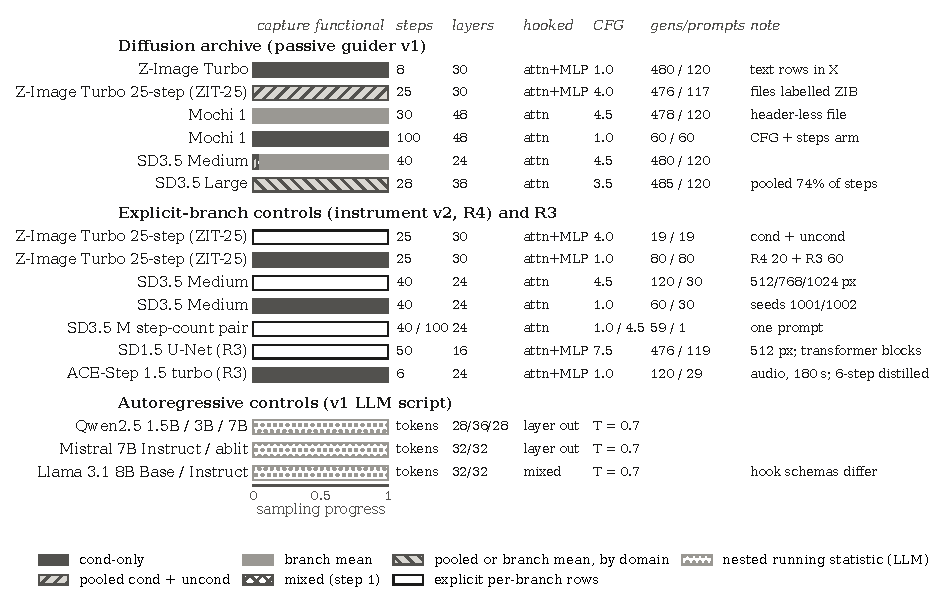
\includegraphics[width=\linewidth]{I-F1_corpus_instrument_map}
 \caption{Corpus and capture instrument. Each row is one campaign. The strip shows which capture functional the stored value records along normalized sampling progress. ZIT-25 is Z-Image Turbo at 25 steps (archive files labelled ZIB). ComfyUI's CFG batching decides this, so it differs between campaigns and can change within a run: cond-only; pooled cond\,+\,uncond; branch mean; pooled or branch mean by prompt domain; explicit per-branch rows (instrument v2); for the autoregressive models, a nested running statistic (the v1 LLM script re-encodes the full context at every token). For the SD1.5 U-Net (\S\ref{sec:unet}), layers are its 16 transformer blocks. The \TT{} archive is pooled throughout; ZIT is cond-only; SD3.5\,M is pooled at step 0, mixed at step 1 and branch-mean from step 2; SD3.5\,L is pooled in 74\% of steps, depending on domain. Columns give steps, transformer layers, hooked submodule, CFG scale and generations/prompts. Every number in this paper names its capture regime.}
 \label{fig:corpus}
\end{figure}

\subsection{Coordinates}
For diffusion models the sampling coordinate is the noise level $\sigma$. The two Turbo campaigns (8 and 25 steps) are compared at equal $\sigma$: the optimal affine time warp between them improves registered correlation by at most $0.005$ over equal-$\sigma$ matching, and per prompt equal-$\sigma$ matching loses at most $0.01$ in 99\% (attention) and 100\% (MLP) of prompts. Every one of 117 shared prompts selects zero layer shift. For one set of weights this is the expected result. Real Base and Turbo are compared at equal $\sigma$ as well. Models of different depth are compared on normalised depth $u$. Because equal $\sigma$ is not equal signal-to-noise across resolutions \citep{hoogeboom2023simple}, resolution comparisons use the SD3 resolution shift \citep{esser2024scaling}: a noise level $t_n$ at resolution with $n$ pixels maps to $t_m=\alpha t_n/(1+(\alpha-1)t_n)$ at $m$ pixels, with $\alpha=\sqrt{m/n}$.

The autoregressive captures are not per-token trajectories: in all seven language-model channels the recorded statistic is perfectly rank-correlated with context length ($|\rho|=1.000$), because it is accumulated over the growing context. We do not use them for any per-token dynamical claim.

\begin{center}
\fbox{\begin{minipage}{0.94\linewidth}\small
\textbf{Estimator definitions used throughout} (formal versions: Mode-II, Definition~8 and Appendix~A).
\begin{itemize}\setlength\itemsep{1pt}
 \item \emph{Depth profile.} For a model at one sampling state, average $(\log g,\log\gap,H)$ over generations at each layer, $z$-score each coordinate across layers, and interpolate linearly onto $n$ equally spaced values of normalised depth $u\in[0,1]$. Leading values use the native grid, $n$ equal to the number of hooked layers of the shallower model of the pair (24, 28 or 30), the smallest grid on which no layer of either model is averaged away; for pairs of equal depth it reads every layer as recorded. The preregistered values use $n=24$, fixed in Round 5 before any lineage data existed; for the 24-layer pairs the two coincide.
 \item \emph{Shape.} Pearson correlation of two flattened $24\times3$ profiles at matched $\sigma$, averaged over states.
 \item \emph{Tangent} $\rho_{\tan}$. Cosine of the first differences along $u$ of the two profiles, with equal weight on the three coordinates, at the nearest $\sigma$ of the second model to each $\sigma$ of the first, averaged over the first model's states. Calibrated only for pairs of equal depth (\S\ref{sec:depthcal}).
 \item \emph{Null p95.} 95th percentile of $\rho_{\tan}$ over random permutations of the second model's layer order (1000 unless stated).
 \item \emph{Identity gate.} Pearson $r$ of the mean-removed depth profiles of mean $\log g$ at the first sampling state (\S\ref{sec:gate}).
 \item \emph{$\beta_{\rm layer}$.} The analyzer's layer step $g_{\ell+1}-g_\ell$, binned against $g$ (\S\ref{sec:topology}).
 \item \emph{Plateau onset.} First $\sigma$ at which population state speed falls below twice its median over $\sigma<0.6$.
 \item \emph{Relative onset.} The $\sigma$ at which held-out seed predictability reaches half of its own final value (\S\ref{sec:seed}).
 \item \emph{VR(4)/walk.} Overlapping-difference four-step variance ratio of seed residual paths, divided by the value the same estimator gives on simulated random walks of the channel's own shape.
\end{itemize}
\end{minipage}}
\end{center}

\subsection{Reproducibility and preregistration}
The archive was analysed in eighteen audit rounds. From Round 2 onward, each round froze its predictions with a SHA-256 hash and a UTC time before any calculation \citep{nosek2018preregistration,simmons2011false}; preregistered and post hoc results are labelled throughout. Rounds 5 and 6 scored $13/9$ and $17/5$ (confirmed/refuted). Round 7 was a release audit of existing outputs; its eight checks are consistency checks, not new predictions. Rounds 11--14 were frozen before their captures or before any statistic was computed on them; Round 12's thresholds were set with an exploratory Base run in view, which its preregistration discloses, and Round 12 was frozen before any of the Round 11--12 Base captures (Z1, Z2) existed. Round 15 was frozen at 21:23:24 UTC on 2026-11-05; its scoring script was saved at 21:24:31 and run once, at 21:24:33--21:26:37, and no threshold was changed afterwards. Its rules were written after exploratory looks (X1--X4) at overlapping cubes, so R15-1, -2, -3, -6 and -7 are tests on captures those looks did not use, while R15-4 and R15-5 add new nulls and resampling to tangent values that were already known; they are not out-of-sample tests of those values. Rounds 16, 17 and 18 were frozen before their captures existed (2026-11-06 15:05, 2026-11-07 22:07 and 2026-11-09 10:32 UTC); Round 18's activation-baseline addendum was frozen at 12:42 UTC the same day, and its two data-handling amendments (float16 overflow in stored sketches, and an eigen-solver that failed to converge) were written after the analysis stopped and before any affected value was seen. Preregistration covers only what was written down: analyses explored and never frozen leave no trace. We apply no multiplicity correction across the 253-row ledger; the seven permutation $p$-values behind the primary claims are summarised descriptively with a Benjamini--Hochberg adjustment (Table~\ref{tab:primary}). Of the 253 scorecard rows, 197 were scored, 8 are consistency checks, and 48 were not scored: 34 were not scorable as captured, and 14 are gates, rule outputs, descriptive or report-only rows, or predictions that were not run. The post hoc layer is larger: 56 numbered review checks (RC1--RC56, of which RC50--RC52 were not run) and four exploratory analyses (X1--X4), whose output tables hold about 2{,}800 result rows. It was not counted as a family, so a family-wise correction of it is not possible; post hoc results are hypotheses unless a later round replicated them. Table~\ref{tab:confirm} separates the confirmatory core: the tangent and baseline predictions frozen before the captures they were scored on existed. The gates named in \S\ref{sec:limits} are the project's standing requirements for claims it does not make: G1, a response measurement under finite perturbation; G2, an independent distillation pair with quality labels; G3, cloned continuations for commitment; G4, context-invariant language-model statistics. Appendix~\ref{app:prereg} lists all scorecards, and every refuted prediction is reported.

\begin{table}[htbp]
\centering\scriptsize
\caption{Confirmatory core: tangent and baseline predictions frozen before the capture they were scored on existed (attention unless marked; 24-point grid, as preregistered). Each is a threshold rule, so no $p$-value or multiplicity correction applies; the falsifier is the rule's failure. Lineage rule: tangent at least the layer-permutation p95 plus $0.30$. Of nine tangent predictions, two were refuted. Everything else in this paper is preregistered with lookahead, on explored data, or post hoc (Table~\ref{tab:primary}).}
\label{tab:confirm}
\setlength\tabcolsep{3pt}\renewcommand{\arraystretch}{0.9}
\begin{tabularx}{\linewidth}{@{}>{\raggedright\arraybackslash}p{1.7cm}L>{\raggedright\arraybackslash}p{3.3cm}>{\raggedright\arraybackslash}p{1.9cm}@{}}
\toprule
Test & Prediction (rule) & Observed & Outcome\\
\midrule
R12-6 on R14 capture & ACE-Step Base$\leftrightarrow$turbo meets the lineage rule, attention and MLP & $0.850$ / $0.572$ (MLP bound $0.542$) & holds\\
R16-1 & same turbo weights across two sessions $\ge0.94$ & $0.918$ / $0.821$ & refuted\\
R16-2 & ACE-Step lineage at turbo's release setting (8 steps) meets the rule & $0.795$ / $0.594$ & holds\\
R17-1 & unrelated PixArt-$\Sigma$$\leftrightarrow$Cosmos in the bottom tier ($\le0.47$), attention and MLP & $0.303$ / $0.687$ & refuted (MLP)\\
R17-2 & rule output for the SD3 Medium$\leftrightarrow$SD3.5 Medium successor & $0.926$ & middle tier\\
R18-1 & documented SD3.5 Large$\leftrightarrow$Large Turbo meets the rule and is $\le0.95$ & $0.818$ (bound $0.601$) & holds\\
R18-2 & SD3.5 Large across sessions $\ge0.95$; cond$\leftrightarrow$uncond $\ge0.90$ & $0.994$; $0.994$ & holds\\
R18-3 & second Turbo session at the same-weights level & $1.000$ & holds (exact replay)\\
R18-4 & Base at shift 6$\leftrightarrow$Turbo within $0.10$ of shift 3 and meets the rule & $0.649$ / $0.682$ & holds\\
R18 B1--B4 & activation CKA: related above its null (B1); separates related from unrelated (B2); tangent's order (B3); distillation below same weights (B4) & B1 yes; AUC $0.968$; Spearman $0.70$; $0.625>0.612$ & 1 holds, 2 not supported, 1 refuted\\
R15 (held-out) & five tests on captures the exploratory looks did not use (R15-1, -2, -3, -6, -7) & see \S\ref{sec:content}, \S\ref{sec:seed} & 4 hold, R15-3 refuted\\
\bottomrule
\end{tabularx}
\end{table}

%=====================================================================
\section{A low-dimensional backbone}\label{sec:backbone}

For each model we stack the population depth profiles of $(\log g,\log\gap,H)$, standardised across depth at each sampling state, into a states$\times$features matrix and compute its principal components. PC1 explains $0.71$--$0.90$ of the variance and the effective rank is $1.5$--$2.5$ (Fig.~\ref{fig:backbone}); the Round 1 reproduction with the entropy effective rank gives $0.74$--$0.89$ and $1.53$--$2.37$, and definition variants move these by about $0.05$. Turbo has eight states, so its rank is at most seven by construction. As a null, every time slice's depth profile is independently circularly shifted along depth, which keeps each profile's smoothness but breaks its registration across steps; all five archive campaigns (four models) beat all 999 null campaigns ($p=0.001$), whose mean effective rank is $4.9$--$14.8$. The low rank therefore comes from depth profiles that stay registered across sampling steps, not from smoothness of individual profiles. The shifts are drawn independently per slice on purpose: one common shift for every slice permutes the columns of the states$\times$features matrix and leaves its singular values, hence its rank, exactly unchanged, so it is not a null. The SD1.5 U-Net (\S\ref{sec:unet}, post hoc) has the same backbone: PC1 $0.90$ (attention) and $0.62$ (MLP), effective rank $1.46$ and $2.24$, against null ranks of $11.1$ and $12.1$ ($p=0.001$). The audio model ACE-Step (\S\ref{sec:ace}, post hoc) gives PC1 $0.78$ and $0.56$ and effective rank $2.10$ and $2.73$ against null ranks of $3.9$ and $4.1$ ($p=0.001$ and $0.011$); with six sampled states its rank is at most five. The Round 12 and 14 Base captures give the same picture (post hoc, same null): ACE-Step Base PC1 $0.81$ and $0.71$, rank $1.87$ and $2.27$; real Z-Image Base (Z1) PC1 $0.64$ (attention) and $0.76$ (MLP), rank $2.28$ and $2.10$, $p=0.001$ throughout. The real Base attention falls below the $0.70$ PC1 level that held in every archive channel, as it does in the preregistered Round 11 Base capture ($0.638$; R11-5, refuted in 2 of 20 cells), while every cell still beats its nulls. The four Round 17 models, captured for the tier controls and not analysed for the atlas before, give the same backbone in all six channels (PC1 $0.72$--$0.91$, effective rank $1.40$--$2.21$ against null means of $9.4$--$15.3$, $p=0.001$; post hoc, RC34, Supplement~\ref{supp:posthoc}).

The same holds within every semantic domain: across 68 archive model$\times$submodule$\times$domain trajectories (the real Base captures of Rounds 11--12 are not among them) PC1 is at least $0.70$, and model and submodule identity explain $0.90$--$0.96$ of the variation in rank and slowdown summaries against $0.02$--$0.05$ for domain. This is low dimensionality of the measured spectral representation; it says nothing about the dimension of the hidden-state dynamics.

Along the sampling clock, every channel shows an early high-speed transient at $\sigma\approx1$ followed by a $\sigma$-invariant plateau. The plateau onset, defined as the first $\sigma$ at which population state speed falls below twice its median below $\sigma=0.6$, lies at $\sigma=0.78$--$0.87$ in all eight archive channels (four architectures, CFG 1--4.5, 8--100 steps),\footnote{The location is a property of this rule. With a threshold of $1.5\times$ or $3\times$ the plateau median instead of $2\times$, the eight channels give $0.57$--$0.81$ and $0.79$--$0.93$; moving the plateau window from $\sigma<0.6$ to $\sigma<0.5$ or $\sigma<0.7$ changes the range by at most $0.09$ (post hoc). Comparisons in this section use the $2\times$ rule throughout.} and is tighter in $\sigma$ than in step fraction (spread $0.32$--$0.64$). On the clean SD3.5 Medium conditional-branch captures it moves with resolution, from $0.72$ at $512$ to $0.81$ at $1024$; on the resolution-corrected clock the three resolutions give $0.81$--$0.84$. The SD1.5 U-Net, mapped to the same clock at equal signal-to-noise ratio, reaches its plateau later, at $0.58$ (attention) and $0.67$ (MLP), or $0.73$ and $0.80$ after the resolution shift (post hoc; the comparison depends on that mapping, \S\ref{sec:unet}). Under the $1.5\times$ and $3\times$ rules the eight archive channels span $0.57$--$0.93$, which contains both U-Net mappings, so ``later'' holds only under the fixed $2\times$ rule. The audio model ACE-Step, on its own flow-matching $\sigma$, reaches it at $0.90$ (attention) and $0.80$ (MLP) in the turbo checkpoint, inside the preregistered window $[0.73,0.92]$ (B8, \S\ref{sec:ace}); the window is $0.19$ wide and with six steps the plateau speed rests on a single interval, so this test had little power to fail, and at $0.79$ and $0.85$ in the 50-step Base checkpoint (B8 replayed, Round 14). On the Round 17 models and the real Base the onset spreads further (post hoc, RC36): $0.74$--$0.78$ for SD3 and SD3.5 Medium and PixArt-$\Sigma$ MLP, $0.66$ for PixArt-$\Sigma$ attention and $0.94$--$0.97$ for Cosmos (both on $t=\sigma/(1+\sigma)$), and $0.68$/$0.78$ for Z1; 6 of 10 channels fall in $[0.73,0.92]$, so the archive range describes those models and is not a general constant. At matched $\sigma$, geometry changes by at most $2$--$3\%$ between 8 or 40 and 100 sampling steps (Turbo: $g$ within $1.9\%$, on a four-generation 100-step control; SD3.5 Medium: $3\%$ at CFG 1 and no change at CFG 4.5). That bound holds for the models it was measured on: in ACE-Step turbo the depth tangent between 3 and 10 steps and 8 steps stays at $0.993$ or above in attention but falls to $0.906$ in MLP at 3 steps (Round 16, R16-4 refuted in one of 12 cells). We read the plateau as a qualitative recurrence, an early transient followed by a $\sigma$-invariant plateau in every channel; its location depends on the rule, on resolution and, across schedules, on the clock mapping, so the numbers above are reported with those choices and are not compared without them.

\begin{figure}[t]
 \centering
 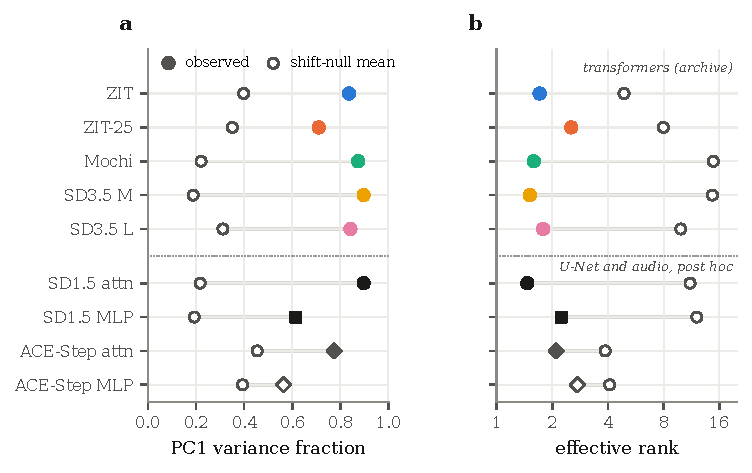
\includegraphics[width=\linewidth]{I-F2_backbone}
 \caption{Low-dimensional temporal backbone in CoS spectral coordinates (descriptive). \textbf{Left:} fraction of variance on the first principal component of the population trajectory, after within-state depth standardization; \textbf{Right:} effective rank; \textbf{Grey markers:} mean of 999 circular-shift nulls, in which each time slice is shifted in depth independently. PC1 is 0.71--0.90 against null means of 0.19--0.40, and effective rank is 1.5--2.5 against 4.9--14.8 ($p = 0.001$ for every model). ZIT has only 8 sampled states, so its rank is at most 7 by construction. \textbf{Below the dotted line} (post hoc): the SD1.5 U-Net, conditional branch, attention (circle) and MLP (square), with the same definition and null: PC1 0.90 and 0.62, rank 1.46 and 2.24 against null ranks 11.1 and 12.1 ($p=0.001$). Diamonds: the audio model ACE-Step (attention filled, MLP open; 6 states): PC1 0.78 and 0.56, rank 2.10 and 2.73 against 3.9 and 4.1 ($p=0.001$, $0.011$).}
 \label{fig:backbone}
\end{figure}

%=====================================================================
\section{Similarity depends on the observable}\label{sec:similarity}

\subsection{Scalar envelopes}
Early in the project, layer-mean attention $g$ along $\sigma$ correlated at $r=0.9405$ between the \TT{} campaign and Mochi, slightly above \TT{} and the 8-step Turbo campaign ($0.9325$), with Turbo$\leftrightarrow$Mochi at $0.8217$. These values reproduce exactly from the archive. The project first read the second value as Base against its own distillation, from the archive label; both campaigns are Turbo, so the example is stronger: the same weights under a different step count, guidance and capture correlate \emph{less} with themselves than with an unrelated video model. Each campaign has a different capture regime (\TT{} pooled, ZIT cond-only). On $\log g$ the same archive gives \TT{}$\leftrightarrow$ZIT $0.973$ against \TT{}$\leftrightarrow$Mochi $0.860$, and with the conditional branch captured explicitly (Round 4, 19 prompts) the linear-$g$ values are $0.989$ and $0.831$ (Fig.~\ref{fig:scalar}). More fundamentally, every denoising trajectory shares a coarse trend in $\sigma$, and a scalar correlation is bounded below by that shared trend whatever the residual dynamics \citep{yule1926why} (Mode-II, trend-dominance proposition). On linear $g$ the best unrelated pair (Turbo$\leftrightarrow$SD3.5 Large, $0.981$) exceeds the same-weights pair ($0.933$).

\begin{figure}[t]
 \centering
 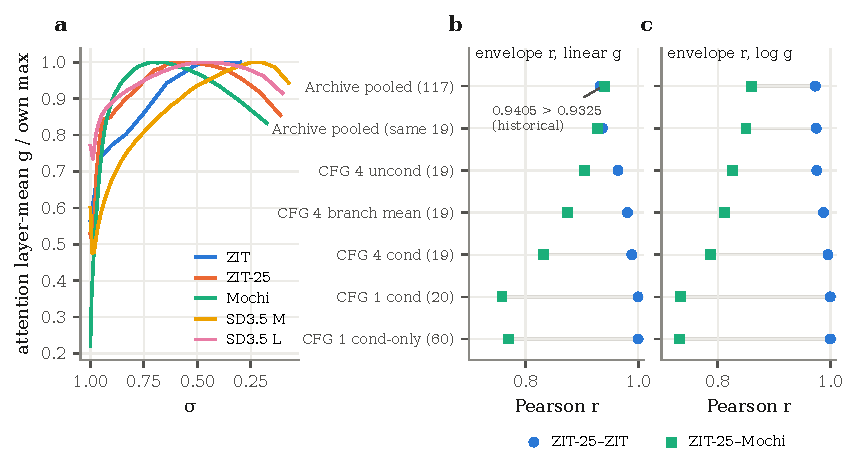
\includegraphics[width=\linewidth]{I-F4_capture_regime_reversal}
 \caption{A scalar envelope ordering that reverses with the capture regime (worked example). Every substitution in the panels is the 25-step Turbo campaign \TT{} (archive files labelled ZIB), so all comparisons are the same Turbo weights. \textbf{(a)} Layer-mean attention $g(\sigma)$, each model scaled to its own maximum. Every envelope rises, so envelope correlations are dominated by a shared monotone trend. \textbf{(b, c)} Correlation of the \TT{} envelope with ZIT (filled) and with Mochi (open) when only the \TT{} capture is substituted, on linear $g$ (b) and log $g$ (c). The historical ordering ZIB$\leftrightarrow$Mochi 0.941 $>$ ZIB$\leftrightarrow$ZIT 0.933 appears only for the pooled archive on linear $g$. It is already reversed on the same 19 prompts. It is reversed in every explicit capture (cond, uncond, branch mean, CFG\,1), and on log $g$ in every capture (archive 0.973 vs 0.860; CFG\,1 cond-only 0.9998 vs 0.732). This is an example of capture-regime sensitivity, not evidence about architecture.}
 \label{fig:scalar}
\end{figure}

\subsection{Fields, shapes and tangents}
We compare model pairs at matched $\sigma$ at four further levels: $\log g$ envelopes, the level field over (depth, $\sigma$), the depth shape (profiles standardised across depth at each state, correlated over a common 24-point depth grid), and the depth tangent (cosine of the first differences of those profiles along depth). Table~\ref{tab:hierarchy} gives, at each level, the margin of the \TT{}$\leftrightarrow$ZIT pair over the best unrelated pair (preregistered, Round 6 S1). Both campaigns are Turbo, so it is the margin of the same weights under changed inference (8 vs 25 steps, CFG 1 vs 4, cond-only vs pooled); the real lineage values follow in Table~\ref{tab:tiers}.

\begin{table}[htbp]
\centering\small
\caption{Same-weights margin by observable level . The first row is \TT{}$\leftrightarrow$ZIT, both Z-Image Turbo.}
\label{tab:hierarchy}
\begin{tabular}{lccccc}
\toprule
 & linear $g$ & $\log g$ & field & shape & tangent\\
\midrule
\TT{}$\leftrightarrow$ZIT (same weights) & 0.933 & 0.973 & 0.984 & 0.981 & 0.942\\
Best unrelated pair & 0.981 & 0.926 & 0.853 & 0.829 & 0.240\\
Margin & $-0.049$ & $+0.047$ & $+0.131$ & $+0.152$ & $+0.703$\\
\bottomrule
\end{tabular}
\end{table}

Registered shape at matched $\sigma$ is $0.981$ (attention) and $0.983$ (MLP) for \TT{}$\leftrightarrow$ZIT on the pooled archive, and $0.9997$ against Turbo at 25 steps and CFG 1 (Round 3); unrelated Z-Image$\leftrightarrow$Mochi shape still reaches $0.79$--$0.83$, so shape alone does not isolate model identity. The tangent does. Within Turbo it depends on the capture in a fixed order: $0.94$/$0.97$ (attention/MLP) for the pooled 25-step campaign against ZIT, $0.981$/$0.989$ for its unconditional branch, $0.988$/$0.991$ for the branch mean, $0.992$/$0.992$ for the conditional branch at CFG 4, and $0.999$ at CFG 1. Read as a decomposition within one model, the step count moves the tangent by about $0.001$, guidance by $0.007$ and the pooled capture by $0.025$--$0.049$. In attention the pooled shortfall sits in the deepest third of the normalised depth grid ($0.86$, against $0.97$ and $0.96$ in the first two thirds), and every third is at least $0.98$ on the conditional capture. The value does not depend on sample size: on 50 prompt-matched subsets of 60 generations it lies at $0.937$--$0.946$ (attention) and $0.965$--$0.968$ (MLP) against $0.942$ and $0.967$ on all generations (preregistered, Round 8 R8-5, R8-6, R8-13). Every unrelated archive pair has $|\cos|\le0.24$, at the 39th--92nd percentile of its own layer-permutation null (95th percentiles $0.24$/$0.20$); all of these pairs differ in depth, so these values are not calibrated levels (\S\ref{sec:depthcal}). The scaling pair SD3.5 Medium$\leftrightarrow$Large gives $-0.25$, a value that changes sign under a depth shift of $0.05$ and is not read as anti-alignment (\S\ref{sec:depthcal}). The tangent is unchanged by any rotation of the hooked activations and by embedding them in a wider space, so a width difference cannot by itself lower it; by the same token, a high tangent is necessary for an orthogonal correspondence between two models' activations but does not establish one (Mode-II, \S4.3). That the same weights stay at $0.94$--$0.999$ across steps, guidance and capture within these campaigns (and at $0.92$ across two capture sessions of ACE-Step turbo, \S\ref{sec:ace16}) means the tangent is insensitive to inference settings by construction, while distillation moves it; whether it grades the size of a weight change or the kind of relation (fine-tuning, LoRA and distillation at matched budgets) needs a dose-response capture (Mode-III).

\subsection{Tiers: same weights, lineage, unrelated}
The real lineage test was preregistered with disclosed lookahead before any real-Base capture existed (Round 12, \texttt{ad06a1bb}, 2026-10-18 06:21 UTC; the thresholds were set with an exploratory 100-step Base run in view, which the preregistration discloses). The Base cubes use the conditional branch and complete generations only. Table~\ref{tab:tiers} gives the result, and ACE-Step adds a second family (Round 14, \texttt{dc997f6d}, frozen after an identity gate and before any other statistic). Both families are depth-matched within each pair (Z-Image 30 layers, ACE-Step 24). Two lineage pairs make this an existence result; both students are few-step models, and the Z-Image Base captures use sampling shift $3.0$ (the official value is $6.0$) to share the 25-step schedule of \TT{} exactly; Round 18 repeats Base at shift $6.0$ (below). A capture of Base and Turbo at matched guidance and seed count is not part of this paper. Two later rounds, both frozen before their captures existed, test the tiers' scope: Round 16 (\texttt{a3b59c92}, 2026-11-06 15:05 UTC) recaptures ACE-Step turbo at its release setting of 8 steps and at 1--10 steps, and Round 17 (\texttt{16ccbe54}, 2026-11-07 22:07 UTC) adds a depth-matched unrelated pair within one modality (PixArt-$\Sigma$ XL$\leftrightarrow$Cosmos-Predict2 2B, 28 blocks each, two labs) and a same-vendor successor pair with no documented distillation relation (SD3 Medium$\leftrightarrow$SD3.5 Medium, 24 blocks each, the same three text encoders; whether SD3.5 Medium was initialised from SD3 Medium is not documented in the material we used, and its MMDiT-X blocks add self-attention to the first 13 layers).

\begin{table}[p]
\centering\footnotesize
\caption{Depth-tangent cosine (attention / MLP) by tier (preregistered: Round 12 for Z-Image, Rounds 14 and 16 for ACE-Step, Rounds 17 and 18 for the controls and the documented distillation pair; ``post hoc'' marks context values). Within each family, rows run from same weights (one checkpoint under changed inference, branch or capture session) through lineage (distillation: a Base model and its distilled student; successor: a later model of one vendor and line; sibling: two models derived separately within one family, Z-Image) to unrelated models. Tiers: an ordering hypothesis (\S\ref{sec:tierstatus}). Notes below.}
\label{tab:tiers}
\scriptsize\setlength\tabcolsep{1.5pt}\renewcommand{\arraystretch}{0.72}
\begin{tabularx}{\linewidth}{@{}Lccccc@{}}
\toprule
Pair & Ev. & Tangent & Subset range & Perm.\ p95 & Surr.\ p95\\
\midrule
\multicolumn{6}{@{}l}{\emph{Z-Image}}\\
Z3 $\leftrightarrow$ ZIT: same weights, two sessions & LA & 0.990 / 0.992 & .985--.991 / .990--.993 & & \\
Turbo R11 $\leftrightarrow$ ZIT, Z3: same weights, 3 sessions & PH & .997--.999 / .997--1.00 & & & \\
Z1 cond $\leftrightarrow$ uncond: same weights, same run & PH & 0.996 / 0.963 & .995--.996 / .961--.963 & & \\
\TT{} $\leftrightarrow$ ZIT: same weights, pooled capture & PA & 0.942 / 0.967 & .931--.949 / .964--.969 & & \\
\textbf{Z1 $\leftrightarrow$ ZIT: sibling lineage, native} & PH & \textbf{0.547 / 0.771} & .533--.560 / .769--.774 & 0.295 / 0.225 & 0.285 / 0.356\\
\quad 24-point grid (prereg., R12-1) & LA & 0.707 / 0.719 & .695--.718 / .716--.723 & 0.292 / 0.198 & 0.345 / 0.335\\
Z1 $\leftrightarrow$ Z3: identical settings, native & PH & 0.547 / 0.760 & .535--.557 / .757--.762 & 0.290 / 0.224 & 0.291 / 0.358\\
\quad 24-point grid (prereg., R12-4) & LA & 0.713 / 0.697 & .703--.722 / .692--.701 & 0.288 / 0.213 & 0.343 / 0.333\\
Z2 (CFG 1) $\leftrightarrow$ ZIT, native & PH & 0.559 / 0.770 & .546--.570 / .767--.772 & 0.290 / 0.225 & 0.281 / 0.352\\
\quad 24-point grid (prereg., R12-5) & LA & 0.714 / 0.718 & .702--.724 / .714--.721 & 0.273 / 0.204 & 0.343 / 0.333\\
\textbf{Z2 $\leftrightarrow$ Turbo R11, image rows, native (primary, MLP)} & PH & \textbf{0.912 / 0.737} & .907--.915 / .733--.740 & 0.226 / 0.203 & 0.370 / 0.285\\
\quad 24-point grid (RC15) & PH & 0.928 / 0.754 & .923--.931 / .749--.758 & 0.249 / 0.225 & 0.414 / 0.348\\
Turbo R18 $\leftrightarrow$ R11 (exact replay, R18-3a); Base shift 6 $\leftrightarrow$ Z1 (R18-4): same weights & OOS & 1.000 / 1.000 & & & \\
\textbf{Base shift 6 $\leftrightarrow$ ZIT: sibling lineage, native} & PH & \textbf{0.520 / 0.760} & .507--.530 / .757--.762 & 0.299 / 0.225 & 0.288 / 0.354\\
\quad 24-point grid (prereg., R18-4) & OOS & 0.649 / 0.682 & .636--.660 / .678--.685 & 0.277 / 0.201 & \\
\emph{cross-depth, not calibrated:} largest unrelated (vs Mochi, SD3.5 M, L; no MLP hooks there) & LA & 0.212 / -- & & & \\
\multicolumn{6}{@{}l}{\emph{ACE-Step}}\\
Base cond $\leftrightarrow$ uncond: same weights, same run & PH & 0.997 / 0.964 & .990--.996 / .941--.977 & & \\
Base GPU 0 $\leftrightarrow$ GPU 1 (other seeds): same weights & PH & 0.992 / 0.972 & & & \\
Turbo 3--10 $\leftrightarrow$ 8 steps: same weights, 1 session (R16-4) & OOS & .993--.999 / .906--.989 & & & \\
Turbo 8 $\leftrightarrow$ 6 steps: same weights, 2 sessions (R16-1) & OOS & 0.918 / 0.821 & .889--.940 / .764--.838 & & \\
\textbf{Base $\leftrightarrow$ Turbo: distillation lineage} & OOS & \textbf{0.850 / 0.572} & .829--.862 / .535--.592 & 0.316 / 0.242 & 0.585 / 0.279\\
\textbf{Base $\leftrightarrow$ Turbo at 8 steps, Base prompts and seeds (R16-2)} & OOS & \textbf{0.795 / 0.594} & .779--.807 / .571--.610 & 0.337 / 0.229 & 0.547 / 0.285\\
\emph{depth-matched unrelated:} vs SD3.5 M, 24 layers each (post hoc, native grid) & PH & $-0.07$ to $-0.11$ / -- & & 0.24--0.34 & \\
\emph{depth-matched unrelated:} 3 ACE-Step vs 3 SD3-family captures (post hoc) & PH & $-0.05$ to $-0.17$ / -- & & 0.30--0.36 & 0.26--0.34\\
\emph{cross-depth, not calibrated:} largest unrelated (vs image models; post hoc) & PH & 0.275 / 0.200 & & & \\
\multicolumn{6}{@{}l}{\emph{SD3}}\\
SD3.5 M in three sessions (archive, Rounds 11, 17; CFG 1, 4.5): same weights & OOS & .980--.994 / -- & .971--.985 (R17-3) & & \\
SD3 M, SD3.5 M cond $\leftrightarrow$ uncond: same run & PH & 0.995 / -- & .990--.994 & & \\
\textbf{SD3 M $\leftrightarrow$ SD3.5 M: successor lineage, no distillation (R17-2)} & OOS & \textbf{0.926} / -- & .918--.932 & 0.260 & 0.397\\
SD3.5 L, Round 18 $\leftrightarrow$ archive: same weights, two sessions, native (R18-2) & OOS & 0.998 / -- & .997--.998 & 0.325 & 0.352\\
\textbf{SD3.5 L $\leftrightarrow$ L Turbo: documented distillation, 38 layers each, native} & PH & \textbf{0.904} / -- & .893--.913 & 0.326 & 0.335\\
\quad 24-point grid (prereg., R18-1) & OOS & 0.818 / -- & .795--.837 & 0.301 & \\
\multicolumn{6}{@{}l}{\emph{Unrelated, depth-matched}}\\
PixArt-$\Sigma$, Cosmos cond $\leftrightarrow$ uncond: same run & PH & .993--.998 & & & \\
\textbf{PixArt-$\Sigma$ $\leftrightarrow$ Cosmos-Predict2 2B: 28 layers each, native} & PH & \textbf{0.196 / 0.572} & .185--.209 / .567--.577 & 0.255 / 0.205 & 0.239 / 0.273\\
\quad 24-point grid (prereg., R17-1) & OOS & 0.303 / 0.687 & .295--.311 / .682--.690 & 0.251 / 0.206 & 0.244 / 0.346\\
\bottomrule
\end{tabularx}
\par\smallskip\raggedright\tiny Empty null cell: not computed. Grid: rows marked native lead (post hoc, RC33): one point per hooked layer of the shallower model (38 for SD3.5 Large, 30 for Z-Image, 28 for PixArt-$\Sigma$ and Cosmos), with 1{,}000 permutation draws, 300 surrogate draws and 200 subset draws; the indented row beneath gives the 24-point value the preregistered rule was scored on. For 24-layer pairs the two grids coincide, and the Z-Image, PixArt-$\Sigma$ and Cosmos same-weights rows move by at most $0.01$ between grids (RC33), so they carry one value. SD3, SD3.5, PixArt and Cosmos hooks read image tokens only, SD3 and SD3.5 attention only; Z-Image values are joint-sequence statistics (image rows: Table~\ref{tab:rowsets}). Subset range: 5th--95th percentile of 200 draws of 30 generations per model without replacement (RC22; R15-5 where it covered the pair). A stability range, not a confidence interval. Null p95: layer-order permutation of the second model (1000 draws; 300 for post hoc rows) and a smoothness-preserving surrogate (300 draws; RC22, post hoc). The first-named model supplies the states (reversing a pair: $\le0.022$). Ev.: evidence class of the row's value, as in Table~\ref{tab:primary} (OOS out of sample; LA preregistered with lookahead; PA preregistered on explored archive data; PH post hoc); the subset ranges are KV (R15-5) or post hoc (RC22). Z-Image MLP all-rows values are caption-row statistics from layer 10 on (Table~\ref{tab:captionmap}), so for Z-Image MLP claims the image-row row is the primary value and the all-rows values are the variant; the Round 12 thresholds were set on all rows.
\end{table}

Every scorable Round 12 test holds: the lineage tangent is above its null (R12-1), at least $0.10$ below the same-weights values (R12-2), at least $0.30$ above the largest unrelated pair (R12-3), and the same at identical settings (R12-4) and at CFG 1 (R12-5). The consequence fixed in advance applies, and the lineage claim is restated as a middle tier: same weights ($0.99$) above lineage ($0.70$--$0.72$) above unrelated models ($\le0.21$, all cross-depth). Because Round 12's thresholds were set with an exploratory Base run in view, the ACE-Step pair (Round 14) is the cleaner out-of-sample test of the tier; the Round 13 holdout covers what distillation changed (below), not the tangent. The ACE-Step pair holds its preregistered test as well (R12-6: tangent at least $0.30$ above the null and at most $0.95$), with an attention value closer to same weights ($0.85$) and an MLP value that clears its bound by only $0.03$ ($0.572$ against $0.542$). Two lineage pairs therefore stand out from passive telemetry, in two modalities, at different strengths: one family in which both submodules clear the tier, and one in which attention does and the MLP clears it only through its last layers. The ACE-Step MLP value is carried by the last layers: with the final depth step removed it is $0.38$, and with the first and last two removed $0.16$, below its null (post hoc). The ACE-Step MLP lineage therefore shares the end-of-depth collapse, not the whole depth profile; per coordinate it sits in the gap (below). One untested hypothesis: few-step distillation, which matches outputs, constrains the last layers most strongly; a layerwise comparison of other distilled checkpoints would test it; Z-Image (both submodules) and ACE-Step attention do not move under the same trimming ($0.70$--$0.78$ and $0.83$--$0.87$). Round 15 (preregistered, \texttt{3acbb027}; frozen 69 seconds before its scoring script ran, and R15-4 and R15-5 add nulls and resampling to values already known) adds two checks. Under a conservative null that permutes layers only within each quarter of depth, and so keeps the coarse depth order, every same-weights and lineage channel stays at least $0.44$ above the null's 95th percentile except ACE-Step MLP ($0.19$), and every unrelated pair stays below it (R15-4). Resampling 30-generation subsets 200 times per pair separates the three tiers of that comparison set without overlap (R15-5). These subset ranges, here and in Table~\ref{tab:tiers}, measure stability under subsampling, not confidence intervals: small subsets lower the cosine, so a range can sit just below the full-sample value; a prompt-level bootstrap gives ranges of similar width centred on the estimate (RC26). This is within-pair stability, not separation of populations: the draws resample the same generations, the 31 channel pairs share models, and the independent lineage observations are two families with two submodules each. Per pair, the 90\% intervals of the draws do not overlap across tiers: the lowest same-weights lower bound is $0.931$ against the highest lineage upper bound $0.862$, and the lowest lineage lower bound ($0.535$, ACE-Step MLP) lies above the highest unrelated upper bound ($0.248$, all cross-depth). That resampling predates Round 17; the depth-matched PixArt-$\Sigma$$\leftrightarrow$Cosmos pair added since gives an attention range of $0.295$--$0.311$ (RC22), which also lies below $0.535$, and an MLP range of $0.682$--$0.690$, which does not. Within each family alone the lowest lineage value exceeds the highest unrelated value (Z-Image $0.70$ against $0.24$, ACE-Step $0.56$ against $0.21$; post hoc). The preregistered AUC of $1.00$ restates this ordering and is not a classification rate. Detecting a derived model from its internal representations is an established problem for language models \citep{zhang2024reef,zhu2025independence,tang2026representations}, parent--child relations between vision networks can be recovered from weights and features \citep{yu2024neural}, and distillation can be detected from weights with teacher access, including in text-to-image models \citep{shi2025knowledge}. What the tiers add is a passive, weight-free reading from three spectral scalars per layer, aligned by sampling state, that separates related from unrelated models among depth-matched pairs and suggests a finer ordering among the related ones (\S\ref{sec:tierstatus}). It is a screen whose false-positive rate is unknown, not a detector: a same-vendor language-model pair without a known distillation relation (Qwen3.5-0.8B$\leftrightarrow$Qwen2.5-1.5B MLP, windowed v2.1 instrument) reaches $0.66$ against a layer-permutation 95th percentile of $0.32$ ($0.44$ against $0.31$ with the last layer dropped; R15-6); no distillation or fine-tuning relation between the two is documented in their releases, and Round 17 finds the same in images (below). ``Lineage'' is therefore used in a broad sense: models from one line of development (vendor, recipe, encoders, depth). Within it we distinguish \emph{distillation lineage} (a Base model and its distilled student: the Z-Image and ACE-Step pairs) from \emph{successor lineage} (a later model of the same vendor and line whose training relation is not documented: SD3 Medium$\leftrightarrow$SD3.5 Medium). Weight-based tests are stronger when weights are available.

\paragraph{The tiers' scope (Rounds 16 and 17, preregistered).} Three results narrow the tiers.
\begin{itemize}
 \item \emph{The ACE-Step pair holds at the release setting.} With turbo at 8 steps on the Base prompts and seeds, Base$\leftrightarrow$turbo is $0.795$ (attention) and $0.594$ (MLP), above the lineage rule (null $0.337$/$0.229$ plus $0.30$) and within $0.06$ of the 6-step values (R16-2, R16-3). No step count from 1 to 10 brings turbo closer to Base ($0.77$--$0.82$ and $0.52$--$0.59$; exploratory).
 \item \emph{Same weights is not one number.} Within one capture session, turbo at 3 to 10 steps matches 8 steps at $0.993$--$0.999$ in attention and $0.906$--$0.989$ in MLP; between the 8-step session and the earlier 6-step session, on the same checkpoint and prompts, the value is $0.918$/$0.821$ (R16-1, refuted against its $0.94$ bar). The gap is present at the first state, where the computation does not depend on the step count (step-0 profile $r=0.926$/$0.863$ between sessions, $1.000$ within; post hoc), so it is a capture-session effect, whose source (conditioning fields, node version or seed design) the logs do not record. Across sessions the attention margin of same weights over the ACE-Step lineage pair shrinks to about $0.12$.
 \item \emph{The middle tier is reached without distillation.} SD3 Medium$\leftrightarrow$SD3.5 Medium, a same-vendor successor that is not a distilled student (whether it continues SD3 Medium's training is not documented), gives $0.926$ against a null of $0.260$ (R17-2: the frozen rule returns ``middle tier'', $0.024$ below its $0.95$ ceiling). It lies above the ACE-Step distillation pair and the Z-Image siblings and level with ACE-Step same weights across sessions. The SD3.5 Medium recapture against the Round 11 capture of the same file, at CFG 4.5 against 1, gives $0.980$, and the ordering of R17-4 holds. The fixed consequence applies: the middle tier marks relatedness in the broad sense above and is not specific to distillation. If SD3.5 Medium continues SD3 Medium's training, its value above the distillation and sibling pairs is what a grading by closeness of training history would predict, which fits the ordering below; the data cannot tell that reading from shared design alone.
 \item \emph{The bottom tier holds in attention only.} PixArt-$\Sigma$$\leftrightarrow$Cosmos-Predict2 2B, unrelated text-to-image transformers of equal depth, gives $0.303$ in attention, just above its null ($0.251$), and $0.687$ in MLP against a null of $0.206$ (R17-1, refuted: the MLP value is above $0.47$, so by the frozen rule the bottom tier did not replicate). The MLP value is inside the lineage range. Most of it comes from the last depth interval, where both MLPs change sharply: without it the value is $0.389$, and without the first two and last two intervals $0.395$ (post hoc). This is the end-of-depth behaviour that also carries the ACE-Step MLP lineage value.
\end{itemize}
\paragraph{A documented teacher--student pair, the session band and Base's shift (Round 18, preregistered).} Round 18 (frozen 2026-11-09 10:32 UTC, \texttt{6db32be7}, before any capture) answers three questions the reviews named. Its gates hold: every arm is complete (SD3.5 Large Turbo after a recapture of four prompts that had failed because its weight file was still a placeholder when the run started), every block is hooked, the step-0 identity checks and the SHA-256 of every weight file separate the checkpoints, and Base's schedule is the shift-6 image of Z1's to $8\times10^{-7}$.
\begin{itemize}
 \item \emph{A documented teacher--student pair sits in the middle tier.} SD3.5 Large against SD3.5 Large Turbo, an adversarial diffusion distillation of it documented by the vendor \citep{sauer2024adversarial}, 38 blocks each, gives $0.818$ on the preregistered 24-point grid against a null of $0.301$ (subset range $0.795$--$0.837$; R18-1 supported: above the lineage rule and at most $0.95$), and $0.904$ on the native grid, $0.58$ above its permutation null and $0.57$ above the surrogate. The same weights across two sessions give $0.998$ (Round 18 against the archive capture, on another prompt set; R18-2) and conditional against unconditional branch $0.997$. This is the third distillation pair and the first whose teacher--student relation is documented. It lies below same weights, $0.022$ below the successor and above the ACE-Step distillation pairs and the Z-Image siblings, so the tangent does not separate a documented distillation from a same-vendor successor. The step-0 identity check reads the pair as $0.986$, inside the same-weights band (\S\ref{sec:gate}).
 \item \emph{A second capture session replays the first exactly.} The second Turbo session used the prompts, seed and settings of the Round 11 session, and its 58 shared generations equal the Round 11 values in every recorded cell; so do all four Round 17 models re-run with activation sketches (60 of 60 generations each). Captures are therefore deterministic at fixed prompt, seed and settings, across sessions. R18-3a ($1.000$ on image rows and all rows) and R18-3b (Z2 against the new session, image rows $0.928$/$0.754$, the values on file) pass by their rules but add no independent measurement, because a session change alone contributes nothing; the preregistration did not anticipate this. The informative band is the prompt set: over 200 random 30/30 splits of the Turbo session the image-row tangent has a 5th percentile of $0.996$ in both submodules, against a 95th percentile of $0.931$ (attention) and $0.759$ (MLP) for Z2 against Turbo on 30 generations each (post hoc). The image-row lineage value lies below that band, which is R18-3c in its informative form.
 \item \emph{The sibling value does not depend on Base's shift.} Base at its official shift $6.0$ against Base at shift $3.0$ gives $1.000$ in both submodules, and against Turbo $0.649$/$0.682$ on 24 points (R18-4 supported: within $0.10$ of the shift-3 values $0.707$/$0.719$ and above the lineage rule) and $0.520$/$0.760$ on the native grid ($0.547$/$0.771$ at shift 3).
\end{itemize}
In attention, on the native grid, the depth-matched pairs order as same weights within a session ($0.98$--$0.999$), same weights across sessions ($0.92$ in ACE-Step, $0.98$--$1.00$ in Z-Image, SD3.5 Medium and SD3.5 Large), a same-vendor successor ($0.93$) and the documented SD3.5 Large teacher--student pair ($0.90$), the ACE-Step distillation pairs ($0.80$--$0.85$), the Z-Image siblings ($0.55$ on all rows; $0.91$ on image rows), and unrelated pairs ($-0.17$ to $0.20$). On the preregistered 24-point grid the siblings read $0.71$ and $0.93$ and the unrelated pairs up to $0.30$. \paragraph{Status of the tiers.}\label{sec:tierstatus} What is measured and what is read into it are kept apart here. \emph{Measured:} among depth-matched pairs, every related pair (same weights, the successor, the SD3.5 Large and ACE-Step distillation pairs, the Z-Image siblings) lies above its layer-permutation null, the Z-Image siblings on all rows by the smallest margin ($0.25$--$0.27$ on the native grid, short of the $0.30$ lineage rule), and every unrelated pair lies at or barely above it. The cross-modal unrelated pairs are inside their nulls and PixArt-$\Sigma$$\leftrightarrow$Cosmos is $0.05$ above it on the 24-point grid ($0.303$ against $0.251$) and below it on the native grid ($0.196$ against $0.255$; $p=0.12$), so the bottom of the scale is better described as indistinguishable from, or barely above, the null than as a calibrated level; with two unrelated pair types the false-negative rate cannot be bounded either. \emph{Read into it, as informed speculation to be revisited:} three tiers within the related pairs, same weights above a close relative above a distillation pair. The Z-Image siblings do not fit one tier: below the distillation pair on all rows and level with the successor on image rows. Their value is still informative: Turbo was distilled from an unreleased SFT model, and Base, the released undistilled model of the family, is not documented as that model or its initialisation (\S\ref{sec:intro}), so the two checkpoints we measured were derived separately, neither from the other, and they share depth dynamics well above both nulls in both submodules on every row set and grid. Three facts keep the tiers a hypothesis. The boundary between the same weights and a close relative is not established: the same ACE-Step weights across two sessions ($0.918$) and the SD3 successor ($0.926$) are level, and on Z-Image image rows the distillation value ($0.928$) fails the R12-2 margin and sits $0.014$ below the pooled-capture same-weights value ($0.942$). The order of the Z-Image siblings and the ACE-Step distillation pair depends on the depth grid (Table~\ref{tab:grid}). And the evidence is six depth-matched related pairs of different checkpoints, one of them (SD3.5 Large and Large Turbo) with a documented teacher--student relation, which sits level with the successor rather than below it. ``Relatedness'' therefore means whatever these pairs share (vendor, recipe, data, encoders, depth); the mechanism is left to tests such as M3-P1 below, and the most informative single result is that a successor with no documented distillation reaches the middle tier, which rules out ``the middle tier detects distillation''. Grouping a distillation pair and a successor in one tier is therefore descriptive: the mechanisms of inheritance differ (output matching against undocumented continued training with changed blocks), and what they share may be macroscopic design (depth, encoders, recipe) rather than a training relation. What would make the tier a measurement is a covariate that moves with it, such as a dose--response along a fine-tuning trajectory or weight-space distance after alignment; neither is in the record. The out-of-sample confirmation of the middle tier is one attention cell (ACE-Step, $0.850$) and one marginal MLP cell ($0.572$ against its bound of $0.542$), plus the successor's rule output, which predicted no direction, and the documented distillation pair ($0.818$, R18-1); Z-Image is preregistered with lookahead (Tables~\ref{tab:tiers} and \ref{tab:cells} give the class of every cell). Round 18 (above) found the documented teacher--student pair in the middle tier, measured the session band where the image-row value sits (a replay; the band is set by the prompt set) and found the sibling value unchanged at Base's official shift. In ACE-Step, distillation is confounded with guidance and step count (Base at 50 steps and CFG 4 against turbo at 8 steps and CFG 1); Z-Image has controls for both axes (Z2, Z3) and its value does not move ($0.707$--$0.714$), ACE-Step has none, so there the tier, not the value, is what survives the confound. For the frozen rules, R12-2 used the pooled \TT{} values ($0.942$/$0.967$) as its same-weights reference, the lower and therefore harder one; R12-4 recomputed it with Z3$\leftrightarrow$ZIT ($0.990$/$0.992$), and the row-set re-scoring of Table~\ref{tab:rowsets} uses split-half references. In MLP the tangent does not separate an unrelated pair from lineage, and every MLP lineage statement in this paper is read with that limit.

\paragraph{Which null defines a tier.} The frozen rules (R12-3, R12-6) are stated against the layer-permutation null, and the tier verdicts are scored that way. The smoothness-preserving surrogate below is the harder null and was added after the fact; under it ACE-Step attention is $0.25$--$0.27$ above the surrogate 95th percentile, short of the $0.30$ margin the frozen rule asks of the permutation null, so that cell passes its preregistered rule and is marginal under the harder null, and is reported as both. From Round 18 on, every tier comparison reports the surrogate margin next to the permutation margin; a rule stated on the surrogate will be frozen for Mode-III. With zero false positives among $n$ independent depth-matched unrelated pairs, the one-sided $95\%$ upper bound on the screen's false-positive rate is about $3/n$, so bounding it at $5\%$ needs about $60$ such pairs, more if pairs share models; the archive has two pair types.

\paragraph{What the screen can and cannot claim (post hoc, review checks RC53--RC56).} Three limits follow from the record, and three checks on the existing captures sharpen them.
\begin{itemize}
 \item \emph{The false-positive rate.} The depth-matched unrelated attention values on file are ten capture pair-directions (PixArt-$\Sigma$$\leftrightarrow$Cosmos and nine ACE-Step$\leftrightarrow$SD3-family combinations), which reduce to five distinct model pairs, because the ACE-Step and SD3-family captures share checkpoints, and to two pair types (Supplement Table~\ref{tab:unrelinv}). None reaches the lineage rule on either grid; one (PixArt-$\Sigma$$\leftrightarrow$Cosmos on 24 points, $0.303$ against $0.256$) lies above its permutation null. With zero false positives among $k$ independent unrelated pairs the exact one-sided 95\% upper bound on the false-positive rate is $1-0.05^{1/k}$: $0.78$ for the two pair types, $0.45$ for the five model pairs, and $0.26$ even if the ten pair-directions were independent, which they are not. The bound is uninformative; the separation is an observation on this set, not an operating characteristic (RC53). At these bounds the screen cannot yet be used as a decision rule in any setting where a false positive is costly.
 \item \emph{Architecture.} The related pairs share more of their architecture (block type, depth, normalisation, conditioning path) than the unrelated pairs, which change several of these at once. The ACE-Step even--odd pattern (\S\ref{sec:ace}) shows that the telemetry does register architecture. Two facts bound this confound without removing it: the successor pair changes its block design (SD3.5 Medium uses a modified block, MMDiT-X, with added self-attention) and stays in the middle tier, and PixArt-$\Sigma$ and Cosmos-Predict2, both 28-block text-to-image transformers, stay at their null in attention. Same-architecture checkpoints trained independently, with and without a parent--child relation, are the decisive test; none is in the record, and it is listed as a Mode-III test (\S\ref{sec:limits}). Until then the result reads: the attention tangent separates the model families tested here from the unrelated architectures tested here.
 \item \emph{Where the separating signal sits in depth.} Expanding each state's depth differences in an orthonormal cosine basis along depth (native grid) and recomputing the tangent per band locates the information (RC54, Supplement Table~\ref{tab:bands}). In the lowest quarter of depth frequencies unrelated pairs agree too ($0.36$--$0.66$ in attention, PixArt-$\Sigma$$\leftrightarrow$Cosmos $0.66$ against a band null of $0.54$), and the Z-Image siblings sit at their band null ($0.655$ against $0.651$). In the middle band related pairs give $0.72$--$1.00$ against unrelated $-0.25$ to $0.36$, and in the upper half $0.46$--$1.00$ against $-0.25$ to $0.01$, so the separation is carried by depth structure with periods of two to eight layers, where most of the difference energy also lies ($41$--$91\%$ in the upper half, periods of two to four layers). A 12-point grid can represent only the lowest 11 coefficients, where PixArt-$\Sigma$$\leftrightarrow$Cosmos reaches $0.56$; this is why the split fails there and holds at 24 points and finer (Table~\ref{tab:grid}), and it is the reason, given after the fact, to read the native grid. Linear interpolation onto 12 points is not an ideal low-pass filter: it also folds part of the unresolvable frequencies back into the resolvable ones, which carries $6$--$35\%$ of the 12-point difference energy. An ideal low-pass applied before resampling gives nearly the same 12-point tangent (correlation $0.96$ over the 17 pair--submodule cells, largest change $0.17$). Without the folding the unrelated attention pairs still rise to $0.49$--$0.65$, against $0.66$--$1.00$ for the related ones, so most of the lost separation comes from the lost frequencies; the folding removes what little gap is left, mainly by lowering the ACE-Step distillation pair from $0.67$ to $0.51$ (RC56, Supplement Table~\ref{tab:recon12}). Two limits apply. The decomposition is of depth differences, which weight fast depth variation up by construction, so RC54 explains how the estimator behaves; it is not a lineage mechanism, and it does not separate training relation from architecture. And the result is post hoc on the pairs that suggested it; confirming it on untouched pairs is a Mode-III test. The native-grid rule (one point per hooked layer of the shallower model) is fixed from here on: it is the primary grid of the first Mode-III preregistration, the architecture control (F-AC1), frozen before its captures exist; it has not yet been tested out of sample.
 \item \emph{Why MLP fails.} Three observations point the same way. The unrelated MLP agreement lies in the lowest depth frequencies ($0.90$ there, which carry $62\%$ of PixArt-$\Sigma$'s MLP difference energy) and in the shared mean direction: centring the statistic lowers PixArt-$\Sigma$$\leftrightarrow$Cosmos from $0.572$ to $0.267$, near its null ($0.211$), while the Z-Image siblings keep $0.523$ against a null of $0.166$, and removing the eight largest channels does not help ($0.757$ unrelated; RC55, RC42; Supplement Table~\ref{tab:mlpvar}). The ACE-Step MLP lineage value is carried by the last depth step (RC22), and the equal weighting of the three coordinates is load-bearing for that one cell (RC18). The MLP tangent on all rows is therefore dominated by terminal-layer and mean-direction structure. A centred MLP tangent separates the two pairs that have centred captures, by $0.26$, which is a hypothesis about a centred MLP screen resting on one related and one unrelated pair, not a result.
\end{itemize}

\paragraph{Robustness of the tiers (post hoc, round-5 review checks RC22, RC24).} Five checks on the existing captures bear on how far the ordering can be trusted.
\begin{itemize}
 \item \emph{A smoothness-preserving null.} Layer permutation destroys the smoothness of a depth profile, so smooth unrelated profiles could beat it easily. In a surrogate that keeps smoothness, the second model's depth-difference profile is phase-randomised along depth with one random phase vector shared by every sampling state and coordinate, which keeps its power spectrum (hence its depth autocorrelation), its registration across states and the coupling of its coordinates. The surrogate 95th percentile is $0.24$--$0.48$ for most pairs and $0.54$--$0.61$ for ACE-Step attention, whose 24-layer profiles are the smoothest (Table~\ref{tab:tiers}). Every related pair stays above it, by about $0.25$ or more (ACE-Step attention $0.25$ and $0.27$, the smallest margins; Z-Image $0.36$; SD3 successor $0.53$); the nine cross-modal unrelated pairs fall inside it; PixArt-$\Sigma$$\leftrightarrow$Cosmos attention ($0.303$) lies above it ($0.244$). The share of surrogate draws that reach the lineage rule (permutation p95 plus $0.30$) is at most $0.05$ for every pair, and the share that reaches $0.47$ is up to $0.17$ (ACE-Step attention). Measured against this null, the ACE-Step attention margin is below the $0.30$ the frozen rule asks of the permutation null.
 \item \emph{Trimming the end layers (MLP).} Removing the first and last two depth intervals, or the first and last hooked layer, does not separate the unrelated MLP pair from lineage: PixArt-$\Sigma$$\leftrightarrow$Cosmos falls to $0.40$--$0.42$, Z-Image lineage stays at $0.74$--$0.76$, and ACE-Step lineage falls to $0.16$--$0.50$, below the unrelated pair. The MLP failure is therefore not an artefact of the terminal block; the MLP tier claim is retired, not repaired. In attention the same trims leave every tier in place; trimming the native end layers lowers the Z-Image lineage value to $0.50$--$0.51$ (same weights $0.99$, unrelated $0.29$), so the Z-Image attention level depends on how the end layers enter the depth standardisation.
 \item \emph{Grid, interpolation and the middle third (RC26, round-6 review).} Table~\ref{tab:grid} gives every tier at depth grids of 12, 24 and 48 points with linear and cubic interpolation, each against its own permutation null. At 24 and 48 points, with either interpolation, every related pair lies above every unrelated pair in attention. At 12 points, coarser than the layer spacing of the 24-layer models, the cross-modal unrelated pairs rise to $0.38$--$0.63$ and PixArt-$\Sigma$$\leftrightarrow$Cosmos to $0.57$--$0.60$, level with ACE-Step lineage ($0.57$--$0.72$): a coarse grid keeps only the large-scale depth shape, which unrelated models share, so the grid is part of the estimator and the separation is a statement at 24 points or finer. The order of the Z-Image siblings and the ACE-Step distillation pair flips with the grid (Z-Image $0.70$--$0.74$ and ACE-Step $0.57$--$0.72$ at 12 points; $0.53$--$0.58$ and $0.79$--$0.86$ at 48), which is one reason the finer ordering is a hypothesis. On the middle third of depth alone (24-point intervals 8--16, $u\approx0.30$--$0.70$), related pairs give $0.65$--$1.00$ and unrelated pairs $0.01$--$0.42$, inside their nulls ($0.38$--$0.47$); the Z-Image lineage margin there is small ($0.65$--$0.67$ against $0.53$--$0.55$). In MLP the middle third removes the ACE-Step lineage value ($0.28$/$0.37$, inside its null) and the PixArt-$\Sigma$$\leftrightarrow$Cosmos value ($0.07$) alike, so the MLP end-of-depth values are end effects in both. A grid tied to the comparison rather than fixed, with as many points as the shallower model has hooked layers (24 for ACE-Step and the SD3 pairs, 28 for PixArt-$\Sigma$$\leftrightarrow$Cosmos, 30 for Z-Image; post hoc, RC30), keeps the split: related pairs $0.55$--$1.00$, unrelated $-0.17$ to $0.20$, PixArt-$\Sigma$$\leftrightarrow$Cosmos now below its null ($0.20$ against $0.26$). But Z-Image attention lineage falls to $0.55$, $0.25$--$0.27$ above both its permutation null and the smoothness-preserving surrogate ($p=0.0003$ with 10{,}000 draws; RC33) and short of the $0.30$ lineage rule, while its MLP rises to $0.77$ and its image-row attention stays at $0.91$. We lead with this grid because it is the one grid size the data fix. Below the number of hooked layers, linear interpolation averages neighbouring layers, a low-pass filter on the very differences the tangent reads, and values become erratic (the 12-point failure above; in a sweep from 12 to 96 points the Z-Image attention value moves between $0.49$ and $0.71$ below 30 points). At or above it, added points carry no new information and values vary less ($0.54$--$0.62$ for Z-Image attention at 30 to 96 points, $0.84$--$0.85$ for ACE-Step attention at 24 to 96; post hoc, RC30). At exactly the hooked-layer count of an equal-depth pair the grid reads every recorded layer once. For pairs of unequal depth no grid gives both models one point per layer, which is the depth-calibration problem (\S\ref{sec:depthcal}). The tangent is thus a family of statistics indexed by grid, interpolation and coordinate weighting, and the separation of related from unrelated pairs is the property shared by the members tested; the tier magnitudes, and Z-Image's place among them, are not. A depth-invariant tangent, one that needs no grid choice, is the central open estimator question (\S\ref{sec:limits}).
 \item \emph{The first state.} Dropping the first sampling state ($\sigma=1$, or $\sigma_{\max}$), where the pooled \TT{} capture carries its largest seed share, changes no tier value by more than $0.015$.
 \item \emph{The session band.} Same weights across capture sessions are tight in two of three families: Z-Image Turbo in three sessions (archive, Round 11, Round 12) gives $0.990$--$1.000$ in both submodules, and SD3.5 Medium in three sessions $0.980$--$0.994$; the ACE-Step turbo value ($0.918$/$0.821$) is the exception. Where the session band is that tight, every lineage value lies far below it. The second Z-Image image-row session (Round 18) replays the first exactly, so the image-row band is set by the prompt set (5th percentile $0.996$ over 30/30 splits) and the image-row attention value ($0.928$) lies $0.07$ below it; against the SD3.5 Medium session band on image tokens ($0.980$--$0.994$) it lies $0.05$--$0.07$ lower, and it lies above the ACE-Step session value.
 \item \emph{Field transfer at matched depth.} A residual vector field fitted on one model and applied to another (Mode-II \S5, re-implemented) transfers between the same Z-Image Turbo weights in two sessions (shortfall $\le0.06$; ACE-Step turbo across sessions $0.23$--$0.25$ in attention) and fails between depth-matched unrelated models (mean cross-model $R^2=-0.33$, shortfall $0.62$), with lineage pairs in between (shortfall $0.37$; post hoc, RC24). The non-transfer between unrelated models is therefore not an artefact of a depth mismatch. Against a same-weights null built from prompt halves (post hoc, RC28), every unrelated and every lineage shortfall has its prompt-bootstrap 5th percentile above the null 95th percentile, and the SD3$\leftrightarrow$SD3.5 Medium successor pair does not (shortfall $0.02$--$0.03$, with a low self ceiling); the shortfall separates same weights from different checkpoints but does not order lineage below unrelated (Mode-II Finding~12).
 \item \emph{Centred and channel-pruned statistics outside Z-Image (post hoc, RC42).} The Round 17 captures store the centred and top-8-removed variants that the archive lacks. On the native grid the successor gives $0.926$ on all rows, $0.848$ centred and $0.911$ pruned, SD3.5 Medium across two sessions $0.980$, $0.953$ and $0.979$, and PixArt-$\Sigma$$\leftrightarrow$Cosmos attention $0.196$, $0.130$ and $0.220$, below its permutation null in every variant. The unrelated MLP value is mostly a shared mean direction: $0.572$ on all rows, $0.267$ centred (permutation p95 $0.199$, surrogate $0.234$), $0.757$ pruned; the last MLP layer of PixArt-$\Sigma$ puts $99.9\%$ of its energy in the mean direction (Cosmos $94\%$; RC43). The attention split survives centring; the MLP bottom tier is reduced by centring, not restored.
 \item \emph{State by state (post hoc, RC49).} Computed at each sampling state instead of averaged, every related attention pair exceeds both its own permutation p95 and the largest per-state unrelated value ($0.252$) at every state (Z-Image siblings $0.385$--$0.693$, rising along the clock; ACE-Step $0.690$--$0.907$; successor $0.889$--$0.952$), and the unrelated attention pairs exceed their p95 at $0$--$5\%$ of states. The separation is therefore not an artefact of averaging over the clock.
\end{itemize}

What distillation changed in Z-Image was found on half of the prompts and then tested on the other, sealed half (Round 13: the six Z-Image predictions held on the holdout; with four ACE-Step turbo predictions that belong to Mode-III, 10 of 10). Base is more concentrated than Turbo: its image-row $g$ is lower at every layer (30 of 30, both submodules), and under identical settings its $g$ is lower at every one of 25 steps; Base image tokens share a larger common mean direction (Base above Turbo in 30 of 30 attention and 29 of 30 MLP layers), and removing that mean shrinks the Base--Turbo difference by $4.3\times$ (attention) and $2.8\times$ (MLP); and the difference sits in the first and last layers, not in the middle (layers 17--22: $0.16$/$0.11$, against $0.60$/$1.09$ early and $1.06$/$0.93$ late). The lower-$g$ direction is not a general signature of distillation: in ACE-Step, Base is below Turbo in only 14 of 24 attention and 10 of 24 MLP layers at matched $\sigma$ (R14-2, refuted).

Two features of the Z-Image capture bear on these values. First, both Z-Image hooks include the 64 caption rows of the joint sequence, whose input comes from the same text encoder in Base and Turbo. Round 11 recorded row-split statistics (Base at CFG 1 against Turbo, 60 prompts), and Table~\ref{tab:rowsets} gives the three tiers per row set (post hoc). On image rows alone the Base$\leftrightarrow$Turbo tangent is $0.928$ in attention and $0.754$ in MLP (all rows: $0.720$, $0.714$); centred, $0.762$ and $0.615$; with the 8 largest channels removed, $0.679$ and $0.435$. Re-scoring the frozen Round 12 criteria on every row set (Table~\ref{tab:rowsets}, last column; post hoc, RC15), the lineage stays above its null and far above the unrelated pair everywhere, and is at least $0.10$ below the same-weights reference in 9 of 10 cells. The exception is the row set this paper recommends as the default: on image rows the attention lineage value ($0.928$) is $0.069$ below the split-half same-weights reference ($0.997$) and only $0.014$ below the pooled-capture same-weights value ($0.942$), so there the attention middle tier is not separated from same weights by the preregistered margin. On image rows, the evidence for a middle tier is Z-Image MLP ($0.754$), ACE-Step attention and the end-layer ACE-Step MLP value. The caption rows do not inflate the lineage value in attention; they lower it. They are not a copy of the shared encoder's output: the hooks read the denoiser's own layers at the caption positions, and on caption rows alone the lineage tangent is $0.70$ in both submodules ($0.699$/$0.703$) against $1.00$ for the same weights. If content shared through the encoder were manufacturing the middle tier, it should be strongest at the caption positions, where the encoder's output enters; it is weakest there, below the all-rows values. Shared encoder content therefore does not raise the lineage tangent in this capture, and encoder sharing is a bounded threat to the Z-Image values rather than an open one; the definitive test is a capture of the encoder's activations with the denoiser fixed (Mode-III). The image-row attention value ($0.928$) is the cell that most needs a reading. One reading, untested and offered as a hypothesis: at image positions, attention is dominated by spatial routing among latent patches, which both checkpoints learn from the same images and the same VAE latent space and which output-matching distillation has no reason to change, whereas the MLPs, which transform per-token features toward a few-step target, change more ($0.754$); in the all-rows capture the caption rows dilute the attention value toward $0.72$. A layerwise comparison of attention maps at image positions would test it; we register it as a Mode-III prediction (M3-P1: on image rows, Base$\leftrightarrow$student attention-map similarity at matched $\sigma$ exceeds the MLP output similarity, layer by layer, in both distillation families). The predictions that image rows and centring would keep the tangent at $\ge0.95$ and $\ge0.90$ (R11-1, R11-2) are refuted, but their thresholds were anchored on archive values that turned out to be a same-weights pair. Against unrelated SD3.5 Medium the tangent stays inside its null in every variant ($-0.13$ to $0.02$; R11-3), and the lineage margin over it is $0.74$--$0.75$ when centred or pruned (R11-4). Second, the uncentred statistic is dominated by the caption rows in Z-Image MLP from layer 10 on (\S\ref{sec:topology}), so the Z-Image MLP values here are mostly statistics of caption tokens. The dominance is a property of the rows, not of one extreme channel (post hoc, RC9, Round 11 captures): averaged over layers 8--29 the caption rows hold $0.96$ (Turbo) and $0.99$ (Base) of the MLP energy, and at least $0.98$ in every layer from 10 to 26 in both; layers 8 and 9 are transitional ($0.85$--$0.98$) and Turbo's last three layers fall to $0.71$--$0.91$. The largest single channel holds $0.07$--$0.13$ on average and fewer than two channels per layer exceed $100\times$ the median.

\begin{table}[htbp]
\centering\small
\caption{The three tiers by row set (post hoc; Round 11 row-split captures, 60 prompts, Base at CFG 1 against Turbo at 8 steps). Same weights: prompt-disjoint split halves of one capture (Turbo / Base), an upper reference rather than a value under changed inference. Unrelated: against SD3.5 Medium (Turbo / Base; attention only). Null: 95th percentile of 300 layer permutations for the lineage pair. Last column: the frozen Round 12 criteria re-scored on each row set (RC15): R12-1 lineage above its null; R12-2 at least $0.10$ below the lower same-weights value; R12-3 at least $0.30$ above the larger unrelated value (attention only).}
\label{tab:rowsets}
\setlength\tabcolsep{4pt}\begin{tabular}{llccccc}
\toprule
Hook & Rows & Same wts.\ (split-half ref.) & Lineage & Unrelated & Null & R12-1/2/3\\
\midrule
attn & all rows & 0.999 / 1.000 & 0.720 & $-0.09$ / $-0.02$ & 0.29 & \checkmark\,\checkmark\,\checkmark\\
 & image rows & 0.997 / 0.999 & 0.928 & $-0.12$ / $-0.13$ & 0.24 & \checkmark\,$\times$\,\checkmark\\
 & caption rows & 1.000 / 1.000 & 0.699 & -- & 0.28 & \checkmark\,\checkmark\,--\\
 & centred & 0.952 / 0.969 & 0.762 & $0.00$ / $0.02$ & 0.19 & \checkmark\,\checkmark\,\checkmark\\
 & top-8 removed & 0.998 / 0.999 & 0.679 & $-0.07$ / $-0.10$ & 0.26 & \checkmark\,\checkmark\,\checkmark\\
MLP & all rows & 1.000 / 1.000 & 0.714 & -- & 0.23 & \checkmark\,\checkmark\,--\\
 & image rows & 0.998 / 0.999 & 0.754 & -- & 0.23 & \checkmark\,\checkmark\,--\\
 & caption rows & 1.000 / 1.000 & 0.703 & -- & 0.30 & \checkmark\,\checkmark\,--\\
 & centred & 0.990 / 0.994 & 0.615 & -- & 0.22 & \checkmark\,\checkmark\,--\\
 & top-8 removed & 0.998 / 0.999 & 0.435 & -- & 0.22 & \checkmark\,\checkmark\,--\\
\bottomrule
\end{tabular}
\end{table}

\begin{table}[htbp]
\centering\small
\caption{Where the caption rows matter: Z-Image claims by row set (Round 11 row-split captures and RC-checks; post hoc unless marked). In 17 (Turbo) and 21 (Base) of the 30 MLP layers the caption rows hold at least $98\%$ of the uncentred energy, so all-rows Z-Image MLP values in those layers describe 64 caption tokens.}
\label{tab:captionmap}
\begin{tabularx}{\linewidth}{@{}LlL@{}}
\toprule
Claim & Rows used & On image rows / centred\\
\midrule
Tangent middle tier (R12) & all rows & attention $0.93$, within $0.07$ of same weights (fails R12-2); MLP $0.75$ holds; centred holds\\
Base more concentrated than Turbo (R13) & image rows & stated on image rows; centring shrinks it $2.8$--$4.3\times$\\
Turbo MLP clock-axis contraction (S4) & all rows & disappears on image rows, centred and pruned (R11-6, prereg.)\\
Base MLP $+,-,+,-$ at CFG 1 (Z2) & all rows & one crossing on image rows\\
Shared prompt geometry & all rows & holds on image rows and centred (RC16)\\
First-state domain decoding & all rows & holds on image rows, caption rows, centred and pruned ($0.29$--$0.47$, every row set above every baseline; RC45)\\
Seed share, Base vs Turbo & all rows & not recomputed on row sets\\
Identity gate & all rows & Base vs Turbo $0.655$/$0.585$ on all rows but $0.945$/$0.930$ on image rows (undecided band): the separation comes from the caption rows (RC44)\\
\bottomrule
\end{tabularx}
\end{table}

\begin{table}[htbp]
\centering\small
\caption{The four lineage cells (depth-tangent cosine, depth-matched pairs; Z-Image is the sibling pair). Z-Image values: native 30-point grid, with the preregistered 24-point value in parentheses; null p95 on the native grid (RC33); ACE-Step grids coincide. Prereg.: Round 12 criteria R12-1 to R12-5 (Z-Image) and R12-6 (ACE-Step) on all rows. Image rows: Round 11 row-split capture (post hoc; Table~\ref{tab:rowsets}); ACE-Step has no caption rows. Per coordinate: $\log g$ / gap / $H$ alone (post hoc, RC18). Ev.: evidence class of the all-rows value; image-row and per-coordinate values are post hoc. For Z-Image MLP the image-row value is the primary one (caption rows dominate all rows).}
\label{tab:cells}
\setlength\tabcolsep{4pt}\begin{tabularx}{\linewidth}{@{}lllccccL@{}}
\toprule
Family & Hook & Ev. & All rows & Image rows & Null p95 & Per coordinate & Verdict\\
\midrule
Z-Image & attn & LA; PH & 0.547 (.707) & 0.912 (.928) & 0.29 & 0.77 / 0.65 / 0.75 & prereg.\ pass at 24 points; native $0.26$ above both nulls, short of the $0.30$ rule; on image rows (24 points) within $0.07$ of same weights (fails R12-2)\\
Z-Image & MLP & LA; PH & 0.771 (.719) & 0.737 (.754) & 0.23 & 0.61 / 0.82 / 0.64 & prereg.\ pass; passes on every row set and on both grids\\
ACE-Step & attn & OOS & 0.850 & -- & 0.32 & 0.91 / 0.74 / 0.88 & prereg.\ pass (out of sample)\\
ACE-Step & MLP & OOS & 0.572 & -- & 0.24 & 0.88 / 0.22 / 0.97 & prereg.\ pass by $0.03$ ($86\%$ of resamples); $0.38$ without the last depth step; gap below its null\\
\bottomrule
\end{tabularx}
\end{table}

\begin{table}[htbp]
\centering\small
\caption{Attention tangent by depth grid and interpolation (post hoc, RC26; all rows, depth-matched pairs; ranges over the pairs of each group). Lin./cub.: linear or not-a-knot cubic interpolation onto the grid. Mid.\ third: 24-point grid, intervals 8--16 only, with its permutation 95th percentile. Permutation 95th percentiles at 12, 24 and 48 points: $0.28$--$0.52$, $0.21$--$0.39$ and $0.21$--$0.41$ over all pairs. Native: a grid with as many points as the pair's shallower model has hooked layers (24, 28 or 30; post hoc, RC30), a rule tied to the comparison rather than fixed, with its 1{,}000-draw permutation 95th percentile. The grid is part of the estimator: the 24-point column is the preregistered one and the others are the same statistic at other settings, not corrections of it.}
\label{tab:grid}
\scriptsize\setlength\tabcolsep{3pt}
\resizebox{\linewidth}{!}{\begin{tabular}{@{}lcccccccc@{}}
\toprule
Group (pairs) & 12 lin. & 12 cub. & 24 lin. & 24 cub. & 48 lin. & 48 cub. & Mid.\ third (p95) & Native (p95)\\
\midrule
Same weights, one session (9) & .98--1.00 & .98--1.00 & .99--1.00 & .99--1.00 & .99--1.00 & .99 & .98--1.00 (.32--.54) & .99--1.00 (.22--.36)\\
Same weights, across sessions (6) & .98--1.00 & .98--1.00 & .98--1.00 & .98--1.00 & .98--1.00 & .98--1.00 & .98--1.00 (.30--.48) & .98--1.00 (.27--.29)\\
ACE-Step turbo, two sessions & .89 & .89 & .92 & .92 & .92 & .93 & .89 (.50) & .92 (.33)\\
\TT{}$\leftrightarrow$ZIT, pooled capture & .92 & .93 & .94 & .94 & .94 & .94 & .95 (.44) & .95 (.25)\\
Successor, SD3 M$\leftrightarrow$SD3.5 M (2) & .90--.94 & .90--.93 & .90--.93 & .90--.93 & .91--.93 & .91--.93 & .90--.94 (.32) & .90--.93 (.28)\\
Siblings, Z-Image (4) & .70--.73 & .71--.74 & .71--.72 & .71--.72 & .57--.58 & .53--.54 & .65--.67 (.53--.55) & .55--.56 (.29)\\
Distillation, ACE-Step (2) & .57--.72 & .58--.72 & .79--.85 & .79--.85 & .79--.85 & .80--.86 & .86--.87 (.48--.50) & .79--.85 (.31--.32)\\
Unrelated, PixArt-$\Sigma$$\leftrightarrow$Cosmos & .60 & .57 & .30 & .27 & .24 & .19 & .01 (.41) & .20 (.26)\\
Unrelated, cross-modal (9) & .39--.62 & .38--.63 & $-$.17--$-$.05 & $-$.17--$-$.05 & $-$.19--$-$.06 & $-$.24--$-$.12 & .16--.42 (.38--.47) & $-$.17--$-$.05 (.33--.38)\\
\bottomrule
\end{tabular}}
\end{table}

\FloatBarrier
\subsection{The tangent is calibrated for equal depth}\label{sec:depthcal}
The tangent compares first differences of two profiles interpolated to a common depth grid (the native grid of the pair, or the preregistered 24 points). First differences are a high-pass operator, so structure at the scale of single layers, such as the parity zig-zag of ACE-Step, lands on the grid differently at different depths. Every same-weights and lineage pair above is depth-matched; every unrelated image pair is not. We therefore tested the estimator on depth-mismatched copies of the same model (post hoc, review checks RC5--RC7). A model against a copy of itself with every other layer kept, or with its layers resampled to 24, keeps $0.90$--$0.99$. At other depth ratios it does not: Mochi against a 38-layer subsample of itself gives $0.15$, SD3.5 Large against a 30-layer subsample $0.08$, and interpolated copies at 30 or 38 layers $0.53$--$0.64$; at 16 layers the values are $0.31$--$0.81$. The one unrelated pair at matched depth, ACE-Step against SD3.5 Medium (both 24 layers), gives $-0.07$ to $-0.11$ on the native grid without interpolation, inside its null (95th percentile $0.24$--$0.34$). The SD3.5 Medium$\leftrightarrow$Large value of $-0.25$ moves to $+0.34$ and $+0.37$ when one profile is shifted by $0.05$ of depth, so it is a phase effect of the mismatch, not anti-alignment. Smoothing the profiles across depth before differencing restores most self-copies ($0.75$--$0.98$ at a bandwidth of $0.04$--$0.12$ of depth) but lifts unrelated pairs to $0.5$--$0.84$, so the tiers merge: the tangent separates pairs because it is sensitive to fine depth structure, and the same sensitivity makes values across depths uncalibrated. The tiers are therefore stated for depth-matched pairs. The unrelated tier is calibrated in attention by two depth-matched pairs, one cross-modal ($-0.07$ to $-0.11$) and one within images ($0.30$ on 24 points, $0.20$ native, Round 17); in MLP the image pair reaches $0.69$ ($0.57$ native), so there is no MLP calibration of the bottom tier. Cross-depth values are reported, but not as levels.

Within that scope the estimator is stable: it is nearly symmetric (reversing the pair changes no tier value by more than $0.022$), the grid size moves magnitudes by up to $0.25$ and keeps related above unrelated on the native grid and at 24 and 48 points but not at 12 (Table~\ref{tab:grid}), three generations per model already separate the tiers, and on $\log g$ or $H$ alone the order holds in every lineage cell; on the gap alone ACE-Step MLP falls below its null, so the equal weighting of the three coordinates is load-bearing for that one cell (post hoc, RC1--RC3, RC6, RC18; details in Supplement~\ref{supp:tangent}). Table~\ref{tab:cells} collects the four lineage cells.

\subsection{Identity-gate audit behaviour}\label{sec:gate}
The gate compares the depth profile of mean $\log g$ at the first state with a reference (Pearson $r$ of the mean-removed profiles; \texttt{fingerprint\_check.py}). On every labelled pair available (post hoc; Table~\ref{tab:gate}), 22 same-weights comparisons, which change steps, guidance, branch, resolution, seed, GPU or capture node, give $r=0.937$--$1.000$, and eight comparisons of different checkpoints give at most $0.70$; one generation suffices for the pairs tested (200 single-generation draws over the available pairs, so this is a statement about those pairs, not a sample-size rule). Rounds 16 and 17 add three cases. ACE-Step turbo across two capture sessions gives $0.863$--$0.927$, inside the gate's band for same weights but below the archive range; the SD3.5 Medium recapture against Round 11 gives $1.000$; and PixArt-$\Sigma$ against Cosmos gives $0.10$ (attention) and $0.67$ (MLP). SD3 Medium against SD3.5 Medium gives $0.940$: the gate reads two different checkpoints of one vendor as the same (R17-0c failed on that pair; the files differ, since the same-weights recapture gives $1.000$). The gate therefore separates a Base model from its distilled checkpoint and unrelated models from each other, but not close relatives. Its limits belong next to these numbers. The thresholds ($0.95$ and $0.98$ for Z-Image) were written when the mislabel was found, before the 30 comparisons were assembled, so they are labelled points, not a calibration set, and no false-positive or false-negative rate is available; a gate whose edges were written against the same record it is then checked on is at risk of optimistic operating characteristics, which a weight hash removes. The reference chain is internal to the archive, because the weight files' hashes were not recorded at capture time. The gate needs equal layer counts, uses the conditional branch, and was calibrated after the failure it caught; a swap between two closely related checkpoints passes it (SD3 and SD3.5 Medium). In use, we read the gate in three bands: $r\ge0.98$ as the same weights; $0.85\le r<0.98$ as undecided, a close relative or the same weights under a different capture session (ACE-Step turbo across sessions $0.86$--$0.93$, SD3 against SD3.5 Medium $0.94$); and $r<0.85$ as different weights. No pair of different checkpoints in Table~\ref{tab:gate} or Rounds 16--17 reached $0.98$, so no mislabel in the opposite direction was observed, but the bands are not a calibrated classifier. The gate needs only the first sampling state, so its cost is one denoiser evaluation per prompt at $\sigma_{\max}$ with the hook attached, about one twenty-fifth to one fiftieth of a full capture at 25--50 steps; one prompt suffices for the pairs tested, and the 60-prompt version used here is the conservative one. Supplement~\ref{supp:gate} gives the table, the alternative statistics and the resolution sensitivity.

\paragraph{Every pair of captured checkpoints (post hoc, RC27, round-6 review).} To give the bands at least an empirical error count, the check was run on every pair of the 25 separate runs in the record with equal hooked-layer counts (conditional branch; within-run splits left out), each run labelled with the weights the record establishes (the archive ``Base'' campaign as Turbo). In attention, none of the 66 different-checkpoint pairs reaches $0.95$; the three in the undecided band are SD3 against SD3.5 Medium ($0.931$--$0.940$, three SD3.5 Medium sessions), and the rest are at most $0.65$ (Z-Image Base against Turbo $0.64$--$0.66$, ACE-Step Base against turbo $0.17$--$0.34$, PixArt-$\Sigma$ against Cosmos $0.10$). Same weights give at least $0.985$ across runs except the ACE-Step turbo session pair ($0.926$, nine runs of one session against the earlier one). In MLP the 19 different-checkpoint pairs reach at most $0.70$ and same weights at least $0.86$. Leaving any one run out changes none of these counts at the $0.98$ and $0.85$ edges. So in this record the $0.98$ edge has no false positive (0 of 66) and one false-negative session pair (ACE-Step), and the $0.85$ edge admits close relatives (3 of 66). These are counts on correlated pairs that share runs, from a labelled set the gate's edges were written against, not error rates. The check is an audit heuristic: where the weight file's SHA-256 is recorded, the hash supersedes it, and the check remains useful when a run's metadata is wrong or missing, which is how it found the mislabelled campaign. It gives no positive proof that every other attribution in the record is right; it shows that every run sits with its labelled checkpoint and away from the others at the edges above.


\begin{figure}[t]
 \centering
 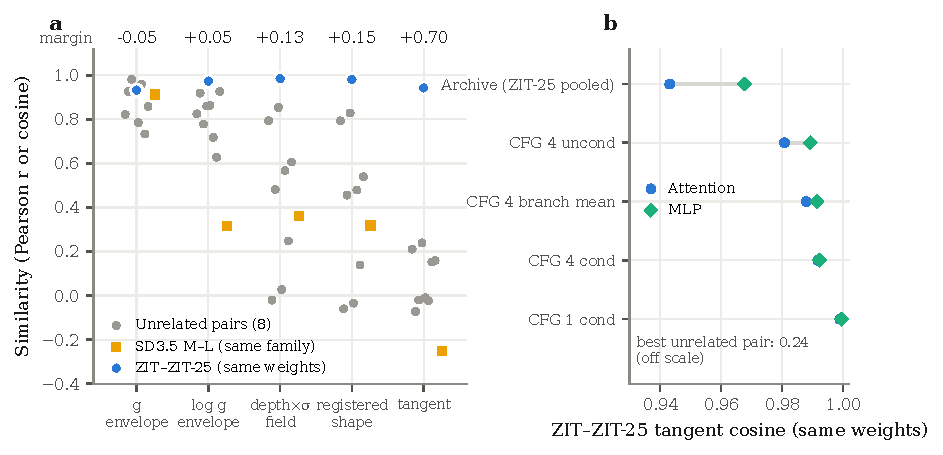
\includegraphics[width=\linewidth]{I-F3_observable_hierarchy}
 \caption{Model identity becomes visible only at the level of the local depth derivative. \textbf{(a)} Similarity of \TT{}$\leftrightarrow$ZIT (the same Turbo weights under changed inference), SD3.5\,M$\leftrightarrow$L (same family) and the eight unrelated pairs, at five observable levels (attention): L0: scalar envelope, linear and log $g$; L1: population field; L2: registered depth shape; L3: matched-$\sigma$ tangent cosine. On the scalar envelope an unrelated pair, ZIT$\leftrightarrow$SD3.5\,L (0.981), beats the same-weights pair (0.933). The tangent separates it: 0.94 against $\le 0.24$ for every unrelated pair. The dashed level marks the real Base$\leftrightarrow$Turbo lineage tangent (0.71 on the preregistered 24-point grid, Round 12; 0.55 native). \textbf{(b)} Tangent of the 25-step Turbo campaign against ZIT under every capture functional, attention and MLP: 0.942/0.967 (archive, pooled), 0.981/0.989 (CFG\,4 uncond), 0.988/0.991 (branch mean), 0.992/0.992 (CFG\,4 cond), 0.999/0.999 (CFG\,1 cond-only). The best unrelated pair is at 0.24.}
 \label{fig:hierarchy}
\end{figure}

\subsection{Aligning states does not align dynamics}
Can unrelated models be made to agree by aligning their state spaces? Procrustes, linear and CCA maps fitted on state landmarks, without derivative labels, visibly improve state alignment between unrelated population fields. Their matched depth derivatives remain near zero or anti-aligned: the best map for each unrelated pair averages a derivative correlation of $0.007$, while the same-weights pair \TT{}$\leftrightarrow$ZIT averages $0.937$ across maps and channels (Fig.~\ref{fig:d10}). The test has not been repeated on the real lineage pair.

\begin{figure}[t]
 \centering
 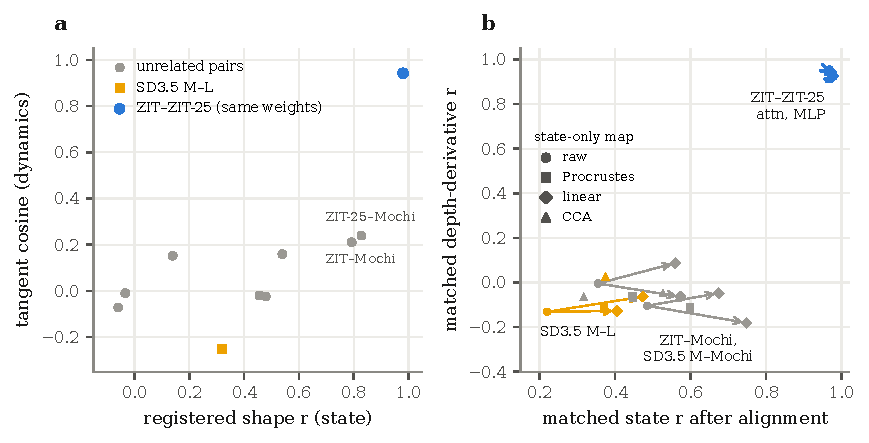
\includegraphics[width=\linewidth]{I-F9_state_vs_dynamics}
 \caption{Aligned states do not imply aligned local dynamics. \textbf{(a)} Registered depth-shape correlation (state) against matched-$\sigma$ tangent cosine (dynamics) for all 10 model pairs (attention). ZIT$\leftrightarrow$Mochi and \TT{}$\leftrightarrow$Mochi have state similarity 0.79--0.83 but tangent cosines of only 0.21--0.24. Only the same-weights Turbo pair is high on both (0.98, 0.94). \textbf{(b)} State-only alignment maps (raw, Procrustes, linear, CCA), learned from state landmarks without derivative labels. They raise the matched state correlation of unrelated and same-family fields (up to 0.75), while the matched depth-derivative correlation stays near zero ($-0.18$ to $0.09$). The same-weights Turbo pair keeps a derivative correlation of 0.92--0.95 under every map.}
 \label{fig:d10}
\end{figure}

\subsection{An activation baseline (Round 18 addendum B, preregistered)}\label{sec:cka}
The reviews asked what the tangent adds over activation-based similarity \citep{kornblith2019similarity,raghu2017svcca}. Addendum B of Round 18 (frozen 2026-11-09 12:42 UTC, \texttt{24a739d4}, before any capture) had the capture node store, for every attention and MLP hook of the conditional branch, the token mean and 36 image tokens at fixed image positions, in float16, at the first state and at the states nearest flow time $0.75$, $0.5$ and $0.25$. It covers the four Round 18 arms, the four Round 17 models re-run, and SD3.5 Medium at CFG 1 as a same-weights reference, on the 60 shared prompts. The primary statistic is linear CKA on token rows (60 prompts $\times$ 36 tokens) for every layer pair, summarised by the symmetric best match ($\tfrac12(\overline{\max_j S_{ij}}+\overline{\max_i S_{ij}})$, which assumes no layer correspondence and so is defined across depth) and averaged over the four states; its null permutes the second model's prompts (200 draws). Attention is primary. Two data-handling amendments were written after the analysis had stopped and before any affected value was seen. Activations beyond the float16 range were stored as infinite in Z-Image (Base: 12 of 30 attention layers at the first state, 2 at the middle states, up to 9 MLP layers), and such a layer is left out of every statistic of that state, in the observed value and in every null draw. The secondary Procrustes similarity is computed from singular values, the same quantity, because an eigen-solver failed to converge.

\begin{table}[htbp]
\centering\footnotesize
\caption{Activation CKA (token rows, best match, mean of four states; attention) against the native-grid attention tangent of the same sessions (Round 18 addendum B; tangent values post hoc). Null: 95th percentile of 200 prompt permutations; every listed pair has $p=0.005$, the smallest possible.}
\label{tab:cka}
\begin{tabularx}{\linewidth}{@{}Lccc@{}}
\toprule
Pair & CKA & CKA null p95 & Tangent (native)\\
\midrule
SD3.5 M at CFG 4.5 $\leftrightarrow$ CFG 1: same weights & 0.612 & 0.385 & 0.984\\
SD3.5 L $\leftrightarrow$ L Turbo: documented distillation & 0.625 & 0.352 & 0.904\\
SD3 M $\leftrightarrow$ SD3.5 M: successor & 0.462 & 0.266 & 0.926\\
Z-Image Base (shift 6) $\leftrightarrow$ Turbo (R18): siblings & 0.344 & 0.132 & 0.521\\
SD3.5 L or L Turbo $\leftrightarrow$ SD3 M or SD3.5 M: same vendor, relation undocumented (4) & 0.367--0.454 & 0.253--0.294 & cross-depth\\
Unrelated, different developers (21) & 0.233--0.364 & 0.133--0.289 & \\
\quad of which PixArt-$\Sigma$ $\leftrightarrow$ Cosmos, depth-matched & 0.338 & 0.243 & 0.196\\
\bottomrule
\end{tabularx}
\end{table}

B1 holds: the same-weights pair and the three related pairs lie above their nulls. By the decision rules, CKA does not separate related from unrelated pairs (B2): the siblings ($0.344$) lie below two unrelated pairs (SD3.5 Medium and SD3.5 Large against PixArt-$\Sigma$, $0.364$ and $0.353$; rank AUC $0.968$). It does not reproduce the tangent's ordering of the five depth-matched pairs (B3: Spearman $0.70$, where five pairs need $0.9$): both put the siblings and the unrelated PixArt-$\Sigma$$\leftrightarrow$Cosmos pair at the bottom, but CKA ranks the documented distillation pair above the same weights at another guidance (B4 refuted, $0.625$ against $0.612$) and the successor below both. Every one of the 21 unrelated pairs also lies above its own prompt-permutation null: that null asks whether two models order the prompts alike, which unrelated image models do (\S\ref{sec:content}), so for CKA ``above the null'' carries no relatedness information, while the tangent's layer-order null places the unrelated pairs at or inside it. Post hoc, the secondary statistics separate the groups in attention, with small margins: CKA at matched depth ($0.326$ against $0.281$), prompt-level and debiased CKA, and Procrustes ($0.863$ against $0.851$); so does the primary statistic without its first state, where the input is noise and Z-Image Base lost the most layers (margins $0.00$--$0.01$ per state). In MLP the Z-Image siblings ($0.239$) lie below PixArt-$\Sigma$$\leftrightarrow$Cosmos ($0.302$). As preregistered, neither instrument is declared the reference. What this shows at this resolution is that the attention tangent's separation of related from unrelated pairs is not a restatement of this coarse activation baseline: CKA ranks the pairs well (AUC $0.968$), which is good discrimination on this set, but the preregistered statistic does not separate them, and the variants that do leave margins of $0.01$--$0.05$, against $0.33$ for the attention tangent (siblings $0.52$ against $0.20$ for the depth-matched unrelated pair), at three scalars per layer and step instead of stored activations. The sketches are coarse (36 tokens, float16, four states), the related pairs are four, and only relatedness was tested; a float32, full-token comparison with matched-depth and best-match variants is needed before any statement about activation similarity in general (\S\ref{sec:limits}).

%=====================================================================
\FloatBarrier
\section{Content geometry}\label{sec:content}

\subsection{Semantic domains are decodable from ordered depth geometry}
A multinomial decoder given only the ordered layerwise profile of $(g,\gap,H)$ at the first measured state recovers the ten prompt domains at $0.45$--$0.61$ with prompt-grouped cross-validation (chance $0.10$; recomputed for this paper with the Round 1 decoder, which gave $0.43$--$0.61$). Layer-averaged scalars give $0.11$--$0.29$ and a prompt-length control $0.15$--$0.18$; a TF-IDF decoder on the prompt text itself reaches $0.38$--$0.42$ (Table~\ref{tab:decode}). Scrambling the layer order within each generation, which keeps every per-layer value, destroys the signal: the real decoder beats all 99 scramble realisations in every channel ($p=0.01$; scramble maximum $\le0.19$). Because the SD3.5 capture regime varies by domain, the decoder could in principle read the regime. On the matched Round 3 captures, where the regime is the same for every prompt, the signal remains (post hoc; 60 prompts, 6 per domain): $0.45$ (attention) and $0.35$ (MLP) for Z-Image Turbo at 25 steps and CFG 1 (cond-only) and $0.32$ for SD3.5 Medium at CFG 1, against a TF-IDF decoder at $0.28$ and a scramble maximum of $0.17$--$0.27$ ($p=0.01$ in every arm); pooled SD3.5 Medium on the same prompts gives $0.29$. Per-domain recall is above chance in every domain and channel except one cell (Fig.~\ref{fig:S5}): abstract and prehistoric prompts are decoded best ($0.71$--$1.00$) and cinematic prompts worst ($0.10$--$0.46$); cinematic prompts describe style and framing more than subject matter, so their domain has the least shared content for the depth profile to carry. The best-decoded domains are also the most lexically distinctive: the text decoder recalls abstract prompts at $1.00$ and prehistoric prompts at $0.50$--$0.67$, so the telemetry's lead over text comes from other domains, most clearly natural landscapes ($0.45$--$0.60$ against $0.00$--$0.08$; post hoc, ZIT, \TT{}, Mochi and SD3.5 Medium attention). The Z-Image channels include the caption rows, which carry prompt identity by construction; the visual-stream channels (SD3.5, Mochi) are the cleaner evidence. The SD1.5 U-Net (post hoc) also beats every scramble, but only at the level of the text decoder: $0.38$ (attention) and $0.42$ (MLP) against TF-IDF $0.40$ (Table~\ref{tab:decode}, Fig.~\ref{fig:decode}). For the audio model ACE-Step the test is not informative: its 29 music prompts give only two or three prompts per domain, so with prompt-grouped folds even the text decoder is at chance ($0.10$), and the telemetry gives $0.11$ (attention) and $0.12$ (MLP). Within regime-homogeneous subsets decoding remains $4.0$--$5.0\times$ chance for pooled SD3.5 Large (9 domains, $0.45$--$0.55$) and $2.3$--$3.4\times$ chance for branch-mean subsets ($0.58$--$0.82$ on 4 SD3.5 Large domains; $0.30$--$0.34$ on 10 SD3.5 Medium domains). Across the seven transformer channels (four models; two pairs of channels are the same Turbo weights), first-state decoding tracks the first-state prompt variance share (Spearman $\rho=0.64$, stable to leaving out any channel; preregistered, Round 9 R9-A4).

\begin{table}[htbp]
\centering\small
\caption{Ten-way domain decoding at the first state (archive regimes; chance $0.10$). Scramble: maximum over 99 layer-order scrambles. \TT{}: the 25-step Turbo campaign; on the real Base captures (Z1, 479 generations) it gives $0.54$ (attention) and $0.46$ (MLP) against scramble maxima of $0.15$ and $0.14$ (post hoc, RC46). Below the line: the SD1.5 U-Net (\S\ref{sec:unet}; post hoc, conditional branch, 476 generations, 119 prompts), same decoder and features. ACE-Step (\S\ref{sec:ace}; post hoc, cond-only, 120 generations, 29 prompts, 2--3 per domain) is not informative: every decoder, including TF-IDF, is near chance.}
\label{tab:decode}
\begin{tabular}{lccccc}
\toprule
Channel & Ordered profile & Layer-averaged & Prompt length & TF-IDF on text & Scramble max\\
\midrule
ZIT attn & 0.548 & 0.285 & 0.175 & 0.410 & 0.167\\
ZIT MLP & 0.554 & 0.190 & 0.175 & 0.410 & 0.135\\
\TT{} attn & 0.489 & 0.191 & 0.168 & 0.406 & 0.139\\
\TT{} MLP & 0.460 & 0.113 & 0.168 & 0.406 & 0.135\\
Mochi attn & 0.609 & 0.283 & 0.159 & 0.412 & 0.140\\
SD3.5 M attn & 0.448 & 0.185 & 0.150 & 0.417 & 0.167\\
SD3.5 L attn & 0.548 & 0.243 & 0.157 & 0.382 & 0.188\\
\midrule
SD1.5 attn & 0.379 & 0.187 & 0.134 & 0.395 & 0.172\\
SD1.5 MLP & 0.424 & 0.183 & 0.134 & 0.395 & 0.187\\
ACE-Step attn & 0.108 & 0.033 & 0.100 & 0.100 & 0.108\\
ACE-Step MLP & 0.117 & 0.067 & 0.100 & 0.100 & 0.175\\
\bottomrule
\end{tabular}
\end{table}

The domains are prompt categories in text-conditioned models. Decoding them shows that the conditioning signal is written into ordered depth geometry; it is not spontaneous class formation of the kind studied in unconditional diffusion \citep{biroli2024dynamical,sclocchi2025phase}.

\begin{figure}[t]
 \centering
 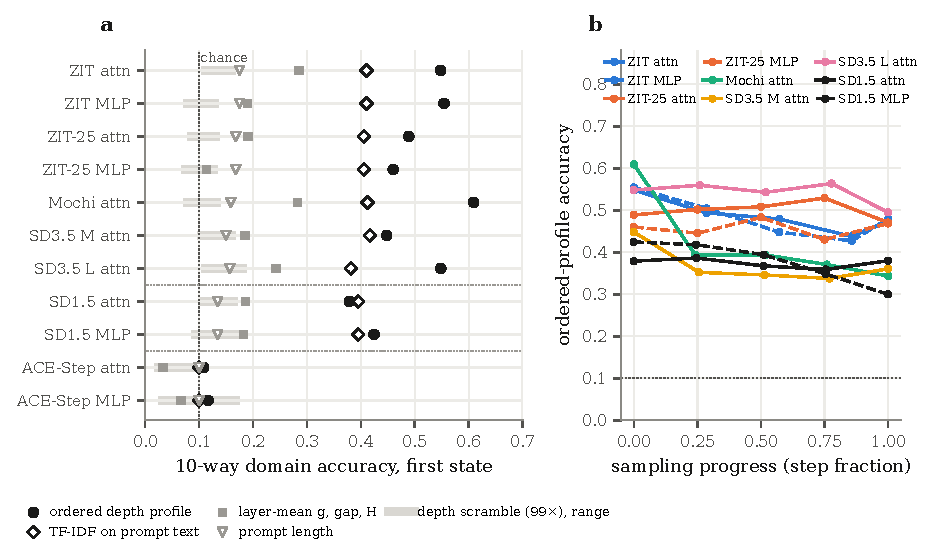
\includegraphics[width=\linewidth]{I-F5_semantic_decoding}
 \caption{Ten-way semantic-domain decoding from telemetry. Decoder: logistic regression on $\log|[g, \mathrm{gap}, H]|$ per layer, 5-fold cross-validation grouped by prompt; chance 0.10. \textbf{(a)} At the first measured state the ordered depth profile reaches 0.45--0.61 across seven channels. This beats: the layer-mean scalars (0.11--0.29); prompt length (0.15--0.18); a TF-IDF decoder on the prompt text itself (0.38--0.42); every one of 99 depth-scrambled realizations (layer order permuted per generation; maximum 0.19, $p = 0.01$). \textbf{(b)} Along sampling the ordered profile stays at 0.34--0.61, above the layer mean in every channel and at every step. Black (post hoc): the SD1.5 U-Net, conditional branch, on 119 prompts. Its ordered profile gives 0.38 (attention) and 0.42 (MLP) at the first state, about the TF-IDF level, and 0.30--0.42 along sampling, still above its layer mean (0.14--0.19). Diamonds in (a), right of the second line: ACE-Step (audio; 29 prompts, 2--3 per domain), where every decoder including TF-IDF is near chance, so the test is uninformative.}
 \label{fig:decode}
\end{figure}

\subsection{A weak but reliable prompt-relational component is shared across models}
For each model and sampling state we form the matrix of distances between prompt-mean depth profiles and compare models by representational similarity analysis \citep{kriegeskorte2008representational} with Mantel permutation tests \citep{mantel1967detection}. The prompt-relational structure is shared across all five archive campaigns (preregistered, Round 6 S2): Mantel $\rho=0.13$--$0.43$ for unrelated pairs and $0.56$--$0.62$ for the two Turbo campaigns (same weights), every $p\le0.0005$. It persists within themes (29 of 30 cells), after partialling out prompt-text overlap (TF-IDF vectors with scikit-learn defaults, no stop-word removal and $\ell_2$ normalisation; distance one minus cosine; the same text representation decodes domains at $0.38$--$0.42$, so it is not a weak control of wording), and after partialling out prompt length (partial Mantel on character-length differences: partial over full $\rho\ge0.998$ in all 24 unrelated-pair cells, so length removes at most $0.2\%$ of the effect, every $p\le0.0001$; preregistered, Round 8 R8-12). Shared text encoders do not explain it: Z-Image$\leftrightarrow$Mochi ($0.39$) exceeds SD3.5 Medium$\leftrightarrow$Large ($0.31$), which share encoders (a refuted prediction, S2e). The S2e ordering, preregistered as ``lineage above family'', is therefore an ordering of same weights above family. Each model in it runs at its recommended operating point, and prompt RSA depends on that point: the same SD3.5 Medium weights at CFG 1 (conditional branch) and at CFG 4.5 (pooled) give $\rho=0.75$ at the first step and $0.38$ later (post hoc). Cross-model RSA orderings are therefore statements at default operating points, not architecture or encoder effects independent of them. On the real Base captures (post hoc), Base$\leftrightarrow$Turbo attention gives $\rho=0.61$--$0.67$ at the three steps, at the level of the same weights, against $0.21$--$0.39$ between Base and the unrelated models; the MLP gives $0.34$--$0.45$. This overlaps the same-weights range ($0.56$--$0.62$) by design of the comparison: content geometry does not tier by lineage, while the depth tangent drops to the middle tier (\S\ref{sec:similarity}). The shared geometry is not a caption-row effect: on the Round 11 row-split captures (60 prompts, post hoc, RC16) unrelated Z-Image$\leftrightarrow$SD3.5 Medium attention keeps $\rho=0.11$--$0.32$ on image rows and $0.20$--$0.43$ centred, and the lineage pair $0.41$--$0.62$ and $0.36$--$0.51$ (every $p\le0.006$); the caption rows carry the strongest lineage value ($0.79$--$0.84$). What is shared is relational structure, not coordinates or mechanism. The same test in ACE-Step does not replicate ($\rho\le0.07$, $p\ge0.09$; Round 15, preregistered, R15-3), and it had little power (post hoc, RC23A). With two seeds per prompt, the split-half reliability of ACE-Step Base's prompt geometry is only $0.10$--$0.53$ (Spearman--Brown), against $0.70$--$0.99$ for Z-Image and ACE-Step turbo, so the observable Base$\leftrightarrow$turbo $\rho$ is capped at $0.32$--$0.71$; a true $\rho=0.30$ would appear as $0.10$--$0.21$ against a null 95th percentile of $0.09$--$0.10$. Even the same weights reach only $0.05$--$0.50$ (Base, two GPUs with different seeds) and $0.06$--$0.23$ (turbo across two sessions). We read R15-3 as an open non-replication with low power, not as evidence against shared geometry in audio. Shared geometry does not mean shared coordinates: a domain decoder trained on one model's first-state attention profiles transfers between the Turbo captures ($0.40$--$0.83$) and partly between Base and Turbo ($0.22$--$0.39$), but across families it stays at $0.09$--$0.22$ (chance $0.10$; post hoc). Two language models reading the same image prompts (Qwen2.5-1.5B and Qwen3.5-0.8B) share a weak but reliable prompt geometry with Z-Image Base ($\rho=0.09$--$0.14$, every $p=0.001$; R15-7), below every pair of diffusion models. The SD1.5 U-Net shares it too (post hoc, bottom row of Fig.~\ref{fig:rsa}): on the 116 prompts common to all six models its attention gives $\rho=0.11$--$0.35$ against the five transformers, every $p=0.0005$. The language models share it too, at matched context (preregistered, Round 9 R9-B6 and its text-control addendum). The prompt-mean depth profiles are compared at the prompt and at generated tokens 128 and 255, residualised on log context length,\footnote{The prefill value is a single statistic of the full prompt matrix, not a nested running statistic, so the context-clock artefact of \S\ref{sec:falsification} does not apply to it; at tokens 128 and 255 every model is compared at the same context length.} with the Mantel test partialled on context-length and TF-IDF text distance. Mistral 7B Instruct and Llama~3.1 8B Instruct, from different developers with different tokenizers and training data, give $\rho=0.44$--$0.48$ on 118 shared prompts, and the three Qwen2.5 sizes give $0.72$--$0.89$ on 24 prompts, every $p=0.0001$. The text controls remove at most $3\%$ of the effect, as they do for the diffusion pairs (unrelated pairs at the first state $0.23$--$0.38$ under the same two controls, at most $5\%$ removed). Each model's own agreement with the text distance is only $0.11$--$0.23$. Because a language model's measured tokens include the prompt itself, the reading is that unrelated models organise the same text alike, beyond its wording and length.

\begin{figure}[t]
 \centering
 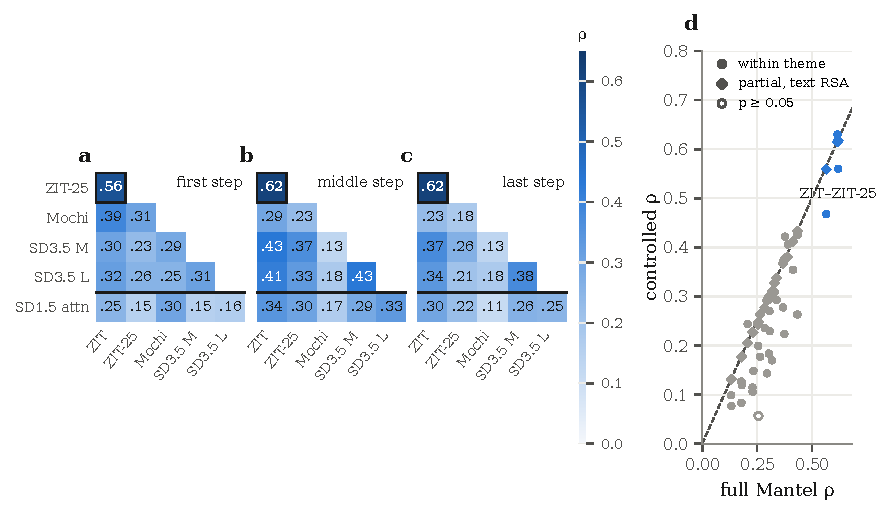
\includegraphics[width=\linewidth]{I-F6_prompt_rsa}
 \caption{Prompt-similarity structure is shared across unrelated models and is strongest for the same weights. \textbf{(a--c)} Mantel $\rho$ between the $117\times117$ prompt-dissimilarity matrices of every model pair at the first, middle and last sampling step. The outlined cell is the two Turbo campaigns (ZIT and \TT{}): 0.56--0.62; Unrelated pairs: 0.13--0.43; Same family (SD3.5\,M$\leftrightarrow$L): 0.31--0.43; Every cell has $p = 0.0005$ against its own 2000-permutation null (null p95 $\approx 0.02$). Bottom row, below the line (post hoc): SD1.5 U-Net attention against each transformer on the 116 prompts shared by all six models (0.11--0.35, every $p=0.0005$); the transformer cells use 117 prompts. \textbf{(d)} Robustness (post hoc). Full RSA against within-theme RSA (theme means removed, theme-preserving null) and against partial Mantel controlling for prompt-text RSA, for all 10 pairs $\times$ 3 steps. The shared structure persists within themes and after the prompt-text overlap is removed. Operating points (archive captures, pooled where guided): ZIT 8 steps CFG 1; \TT{} 25 steps CFG 4; Mochi CFG 4.5; SD3.5\,M 40 steps CFG 4.5; SD3.5\,L 28 steps CFG 3.5; each value holds at these points only, since RSA moves with the operating point (\S\ref{sec:content}). Partial Mantel tests can be anti-conservative under autocorrelation; a multiple-regression-on-distance-matrices check is listed as open.}
 \label{fig:rsa}
\end{figure}

\subsection{Variance shares}
Across the archive, the system$\times$time scaffold accounts for $96\%$ of normalised depth-geometry variance and theme, prompt and seed for the remaining $4\%$. That share is mostly between models and between sampling states. Within a fixed (model, state) cell, prompt identity explains $51\%$--$96\%$ of the variance as a naive share (between-prompt over total sum of squares) and $36\%$--$95\%$ after correcting for seed replication (the one-way random-effects ANOVA estimate $\hat\sigma^2_{\rm prompt}=(\mathrm{MS}_{\rm between}-\mathrm{MS}_{\rm within})/n_0$, with $n_0$ the effective number of seeds per prompt, as a share of $\hat\sigma^2_{\rm prompt}+\mathrm{MS}_{\rm within}$, summed over standardised features and layers); the lowest values are \TT{} at $\sigma=1$, where the pooled first step carries a large seed share. The SD1.5 U-Net falls inside both ranges ($0.67$--$0.75$ naive, $0.56$--$0.67$ corrected; post hoc). The audio model ACE-Step lies at the top in its turbo checkpoint ($0.86$--$0.97$ naive, $0.82$--$0.96$ corrected); its share is highest at $\sigma=1$ and dips at $\sigma=0.60$, so it does not rise first as in every image channel (B10, refuted; \S\ref{sec:ace}). The 50-step Base checkpoint, with two seeds per prompt at CFG 4, has a much lower share ($0.59$--$0.75$ naive, $0.22$--$0.52$ corrected), and its share does rise first (B10 holds; Round 14). Both statements are true, and the second is the relevant one for content.

\paragraph{Prompt content reaches the unconditional branch early.} With explicit branches, the unconditional forward never sees the prompt; it can differ across prompts only through the latent the guided sampler has written. Its prompt geometry therefore times the transfer of content from the text input into the latent. In Z-Image Base the first-state domain decoder reads the conditional branch at $0.54$ (attention) and $0.46$ (MLP) and the unconditional branch at chance ($0.08$, $0.11$), as it must. One step later ($\sigma=0.986$) the RSA between the two branches is $0.61$ in attention, rising to $0.90$ by $\sigma=0.82$ and $0.97$ at the end, and the unconditional branch decodes the domain at $0.24$, rising to $0.42$; ACE-Step Base reaches $0.92$ by $\sigma=0.95$ (post hoc). Round 15 tested this on captures with one global seed per arm, where every prompt starts from the same noise, so shared seed noise cannot produce it (R15-1, preregistered): within the first 10\% of steps the branch RSA reaches $0.68$ (SD3.5 Medium), $0.81$--$0.83$ (Z-Image Turbo at 25 steps) and $0.67$--$0.85$ (SD1.5 U-Net), from $\le0.12$ at step 0, and ends at $0.80$--$1.00$ (four of five channels meet every threshold; Turbo MLP ends at $0.797$ against $0.80$). Prompt-specific internal geometry is thus in the latent within the first few percent of the noise schedule, in all three architectures and in audio. This bears on when guidance can act: \citet{kynkaanniemi2024applying} find guidance harmful at the highest noise levels and most useful in a middle interval, and our data show that by the start of that interval the prompt-specific geometry is already in the latent.

\subsection{Theme residuals}
After removing each model's scaffold, the alignment of theme residuals between models is strongest for the two Turbo campaigns at every state ($0.678$, $0.750$, $0.626$ at the first, middle and last states), but unrelated pairs reach $0.48$ by the middle state and $0.52$ at the end, while at the first state they lie at $0.07$--$0.22$. Theme alignment is specific to the same weights only at the first state (Fig.~\ref{fig:S1}); whether theme alignment is shared under distillation is not tested. Across the ten pairs with both measurements, content similarity and tangent similarity are not detectably rank-coupled (Spearman $0.297$, $p=0.41$; a low-powered test).

%=====================================================================
\section{Sign structure along two axes}\label{sec:topology}

The archive supports two different three-segment statements. They are measured on different axes and are reported separately.

\subsection{Along the sampling clock: Z-Image Turbo MLP}
Layer-mean MLP $g$ in Z-Image Turbo follows expansion, contraction (by about $50\%$) and re-expansion as $\sigma$ decreases. A two-breakpoint piecewise-linear fit \citep{muggeo2003estimating} recovers the order $+,-,+$ in 1000 of 1000 prompt bootstraps, on the archive and on clean explicit-branch captures at CFG 1 and CFG 4 (preregistered, S4). For the 25-step channel no time-order permutation fits comparably (0 of 1000 in all three captures); the 8-step channel's eight states are too few for that test (38 of 1000). Every one of these captures is Turbo. The real Base MLP does not contract: the preregistered prediction that it would show $+,-,+$ in at least $90\%$ of bootstraps fails in every variant (R11-6: $+,+,+$ for all rows, image rows and centred statistics, $+,+,-$ with the 8 largest channels removed; $+,-,+$ in $0\%$), and the primary Base capture Z1 gives $+,+,+$ as well (post hoc). Within Turbo, the contraction is carried by the caption rows: it holds for all rows in $100\%$ of bootstraps and disappears in image rows, centred and pruned statistics (R11-6). From layer 10 on, the 64 caption rows carry at least $98\%$ of the uncentred MLP energy in every layer up to 26 in both Base and Turbo (layer means over 8--29: $0.96$ Turbo, $0.99$ Base; RC9), and $40$--$100\%$ in deep attention layers (R11-7: the prediction that they stay below $10\%$ fails in $56$--$79\%$ of cells); where that share exceeds $0.99$, the all-rows $g$ equals the caption-only $g$. The clock-axis contraction is therefore a property of Turbo's caption-token statistics, not of image tokens and not of the Z-Image family. Attention $g$ instead rises and then falls late, $+,+,-$, in all five archive campaigns (post hoc) and in real Base (Z1, post hoc), and in PixArt-$\Sigma$ and Cosmos in both submodules; SD3 Medium and the Round 17 SD3.5 Medium capture, which ran a different sampler (Appendix~\ref{app:provenance}), give $+,+,+$ in every bootstrap (post hoc, RC37), so the late fall is common but not universal. The SD1.5 U-Net (\S\ref{sec:unet}) has MLP hooks, and neither of its envelopes follows either pattern: with the same fit on the matched clock $t=\sigma/(1+\sigma)$, MLP and attention $g$ both rise over the whole schedule, $+,+,+$ in 1000 of 1000 prompt bootstraps (the MLP levels off and ends $0.6\%$ below its maximum), on raw $\sigma$ and on the resolution-shifted clock as well (post hoc; its schedule covers $t=0.94$--$0.12$). The time-averaged MLP depth profile peaks at layer 5, has a floor in the middle layers and rises over the last layers (post hoc, descriptive). The audio model ACE-Step (\S\ref{sec:ace}, post hoc) shows neither pattern either: on its six turbo steps both envelopes peak at $\sigma=1$, drop by $16\%$ (MLP) and $19\%$ (attention) at the first step, partly recover and then fall, $-,+,-$ in 1000 of 1000 prompt bootstraps (six points barely constrain a three-segment fit, so this is descriptive). On the 50 Base steps the point fits are $-,+,+$ (attention) and $+,+,-$ (MLP), with $+,-,+$ in none of 1000 bootstraps.

\begin{figure}[t]
 \centering
 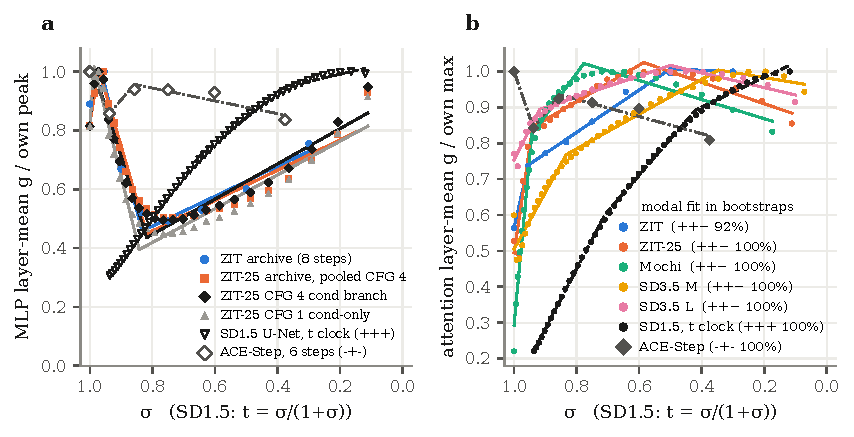
\includegraphics[width=\linewidth]{I-F7_sigma_three_regime}
 \caption{Along $\sigma$, Z-Image Turbo MLP expands, contracts and re-expands; attention does not. All four MLP captures in (a) are Z-Image Turbo; ZIT-25 rows are 25-step Turbo campaigns. Real Base MLP gives $+\,+\,+$ (Round 11, not drawn). \textbf{(a)} Population-mean layer-mean MLP $g(\sigma)$, scaled to its own peak, with the continuous three-segment piecewise-linear fit, for four captures: archive ZIT (8 steps); archive \TT{} (pooled, CFG\,4); the clean 25-step CFG\,4 cond branch; 25-step CFG\,1 cond-only. Every channel gives $+\,-\,+$ in 100\% of 1000 prompt bootstraps, with a contraction of about 50\% ($49.7\%$ in the pooled archive, $50.5\%$--$50.8\%$ in the 8-step archive and the CFG 4 conditional branch, $55\%$--$56\%$ at CFG 1). In the 25-step channels 0/1000 time-order permutations fit comparably; ZIT's 8 points cannot carry that test (38/1000). \textbf{(b)} The same fit on attention in all five models gives $+\,+\,-$ (a rise followed by a late fall), in 92--100\% of bootstraps, not $+\,-\,+$. Black, dashed (post hoc): the SD1.5 U-Net, conditional branch, MLP in (a) and attention in (b), drawn on the matched clock $t=\sigma/(1+\sigma)$. Both rise over the whole schedule ($+\,+\,+$ in 100\% of bootstraps), with no contraction and no late fall. Diamonds, dash-dot (post hoc): the audio model ACE-Step (6 steps, cond-only), MLP in (a) and attention in (b): $-\,+\,-$ in 100\% of bootstraps, with the maximum at $\sigma=1$.}
 \label{fig:sigma}
\end{figure}

\subsection{Along depth: the layer step of $g$}
The CoS-PAFS analyzer measures the layer-direction flow as $\beta=g(\ell+1)-g(\ell)$, bins all (generation, step, layer) points of $\beta$ against $g$ into 29 bins with at least 10 points each, and reports the sign pattern and zero crossings of the binned mean. We ran the analyzer's own function, unchanged. The three-crossing pattern $+,-,+,-$ appears in several archive channels, with different surrogate classes (Table~\ref{tab:beta}): in all 100 generation bootstraps for SD3.5 Medium and Large attention, in $90\%$ and $84\%$ for the 8- and 25-step Turbo MLP channels, and in $67\%$ for 25-step Turbo attention. At a single noise level it appears in every archive architecture at some stage of sampling: SD3.5 Large in 24 of 28 steps ($\sigma$ from $0.96$ to $0.19$), Mochi in 18 of 30, SD3.5 Medium in 13 of 40 (early, $\sigma\ge0.86$), 25-step Turbo MLP in 9 of 25 and 8-step Turbo MLP in 3 of 8.

It is not a property of the Z-Image family or of image data. With the same analyzer function and 100 prompt bootstraps (Round 12, R12-8, descriptive), the real Base conditional branch has one crossing in attention (modal in $50\%$ of bootstraps; three crossings in $11\%$) and in MLP ($100\%$), and so does Turbo run at Base's settings (Z3, $100\%$ in both). At CFG 1 the Base MLP all-rows cloud (Z2, 60 generations; Round 11 recapture, descriptive) does have three crossings, in $74\%$ of bootstraps, but on image rows alone it has one crossing in $100\%$, so there the sequence comes from the caption rows. In the 25-step pooled Turbo campaign the pattern is modal in $59\%$ (attention) and $69\%$ (MLP) of prompt bootstraps, and in the 8-step campaign's MLP in $65\%$. Only the Base unconditional branch gives a three-crossing point estimate in attention ($44\%$ of bootstraps). The same Turbo weights therefore show or lose the pattern with step count, guidance and capture, and the Base weights show it only in the CFG 1 MLP cloud, through the caption rows. In SD3.5 Medium, the Round 11 recapture keeps it on all rows ($98\%$) and with the 8 largest channels removed ($100\%$), and loses it when the activations are centred ($0\%$): it is a property of the uncentred moment, i.e.\ of the shared mean direction.

Two surrogate classes and a step-joint null qualify the pattern (Supplement~\ref{supp:beta}, Table~\ref{tab:beta}). In SD3.5 Medium attention and in 25-step Turbo attention and MLP neither a marginal nor a mean-field surrogate reproduces it (0 of 1000 draws each), so it requires within-generation coupling across layers; in 8-step Turbo MLP it follows from the mean field; in SD3.5 Large it is null-generic in the pooled cloud but not at about half of its single noise levels. ACE-Step has a single crossing in both checkpoints (B6 refuted). No universal crossing location or interval ratio exists (the middle segment spans $3\%$--$77\%$ of the range), and the crossing count depends on the capture regime, on whether attention and MLP are pooled, on which steps enter the cloud, on sample size and on the number of bins: with the analyzer's computation at 15, 20, 29, 40 and 50 bins, only SD3.5 Large keeps three crossings at every count; SD3.5 Medium, 25-step Turbo and Mochi change between one and three, and 8-step Turbo MLP between three and five (post hoc, RC29). The robust statement is the sign sequence with its bootstrap rate and surrogate class, per channel and per $\sigma$.

\begin{figure}[tp]
 \centering
 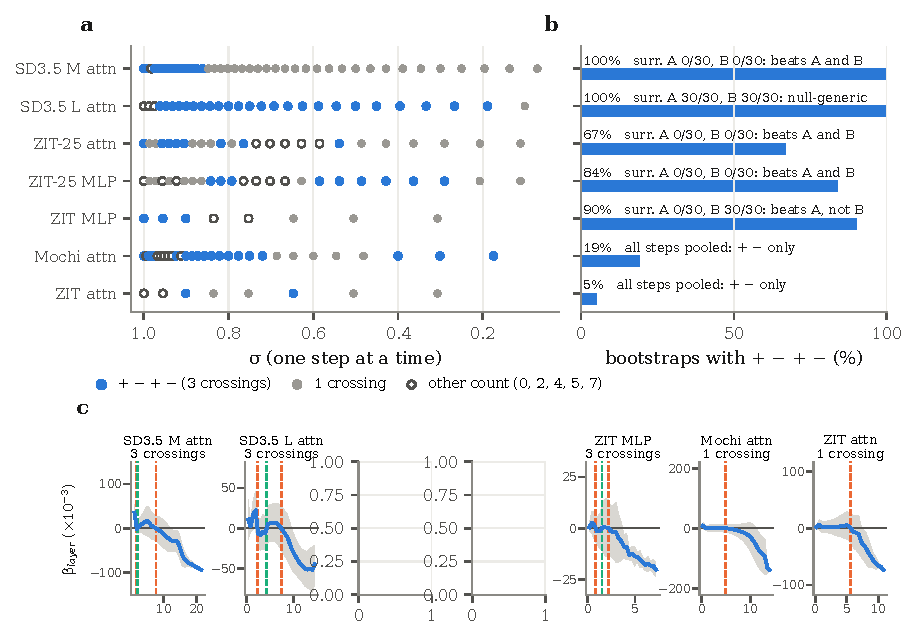
\includegraphics[width=\linewidth]{I-F8_layer_beta_topology}
 \caption{Along the layer axis, the analyzer's layer-direction flow $\beta_{\text{layer}} = g(L{+}1) - g(L)$ shows the $+\,-\,+\,-$ three-crossing pattern in Z-Image Turbo, SD3.5\,M/L and Mochi at some or all $\sigma$ (post hoc analyzer replay). Every Z-Image row is Turbo (ZIT-25 is the 25-step campaign); the real Base conditional branch has one crossing (Table~\ref{tab:beta}). \textbf{(a)} Crossing pattern at each denoising step, one $\sigma$ at a time. \textbf{(b)} Fraction of 100 generation bootstraps with $+\,-\,+\,-$ on all steps pooled: SD3.5\,M and L attention: 100\%; ZIT MLP: 90\%; ZIT-25 MLP: 84\%; ZIT-25 attention: 67\%; Mochi and ZIT attention: 19\% and 5\%. The panel also shows how often marginal (Surrogate A) and mean-field (Surrogate B) surrogates reproduce the observed pattern (30 draws; a 1000-draw rerun gives the same class in every channel, Table~\ref{tab:beta}). The pattern exceeds both surrogates in SD3.5\,M attention and in 25-step Turbo attention and MLP; SD3.5\,L is null-generic. \textbf{(c)} The binned curve $\beta_{\text{layer}}(g)$ itself for each channel, all steps pooled, as drawn by the analyzer's own \texttt{plot\_beta\_layer} (29 bins, at least 10 points per bin; blue: binned mean; grey band: $\pm1$ s.d.; dashed lines: the analyzer's crossings $g^{*}$, orange $+\to-$, green $-\to+$). In several channels the middle segment is narrow compared with the spread across generations. Read the pattern per $\sigma$ or with its bootstrap rate, not as a single crossing count.}
 \label{fig:beta}
\end{figure}

%=====================================================================
\section{Seed predictability without commitment language}\label{sec:seed}

For each sampling step we predict a generation's final seed residual (its state with the prompt mean removed) from its current residual, with ridge regression and prompt-grouped cross-validation, and record the $R^2$ curve $A(t)$.

The usual onset, the $\sigma$ at which $A(t)$ first exceeds $0.5$ ($\sigma_{50}$), turned out to be mostly a sample-size number. The ceiling $A(T-1)$ rises from $0.48$ to $0.89$ as the number of generations grows from 60 to 480, and $\sigma_{50}$ moves with it, from undefined (in 98\% of partitions at $n=60$) to $0.72$ and then $0.94$. An earlier contrast between ``early'' onsets in mixed-regime arms and ``late'' onsets in conditional arms was a comparison across different $n$. Cross-validated estimates at this sample size carry large error bars \citep{varoquaux2018cross}. We therefore use the relative onset, the $\sigma$ at which $A(t)/A(T-1)$ crosses $1/2$, reported at matched $n$ over prompt-grouped partitions. Across channels its range is $0.277$, against $0.501$ for $\sigma_{50}$, and its interval is narrower in 7 of 7 channels (preregistered, S3; Table~\ref{tab:seed}). Relative onsets lie at $\sigma=0.84$--$0.95$ (Turbo MLP $0.67$), and guidance shifts them by at most $+0.03$. Operationally, the relative onset is the noise level by which passive telemetry has reached half of its own final linear predictability of a seed's final residual; it says when the outcome becomes linearly readable from the spectra, not when it is decided: $A(t)$ is a linear-readability curve, and ``onset'' here never means commitment. The ridge penalty ($\alpha=100$, fixed in Round 6) matters little: for $\alpha$ from $10$ to $1000$ the onsets move by at most $0.06$ and the order of the seven channels is kept (Spearman $1.00$ and $0.93$ with $\alpha=100$); at $\alpha=1$ or $10^4$ they move by up to $0.11$ and $0.23$ (post hoc, RC23B). The ratio removes the ceiling's dependence on $n$ only to first order, so relative onsets are compared at matched $n$; a channel with few generations needs its ceiling estimated from as many generations as its comparison partner. It is not the plateau onset of \S\ref{sec:backbone}: the two do not order the channels alike (Spearman $0.56$, below the preregistered $0.7$; Round 10 R10-2).

\begin{table}[htbp]
\centering\small
\caption{Seed predictability at matched $n$ (60 prompts, 50 prompt-grouped subsets, archive regimes): median and 5--95\% interval. VR4/walk: four-step variance ratio divided by its simulated finite-walk value. \TT{}: 25-step Turbo.}
\label{tab:seed}
\begin{tabular}{lccc}
\toprule
Channel & Relative onset & $\sigma_{50}$ & VR4/walk\\
\midrule
ZIT attn & 0.841 [0.798, 0.867] & 0.514 [0.396, 0.608] & 1.13\\
ZIT MLP & 0.673 [0.627, 0.707] & 0.413 [0.362, 0.459] & 0.65\\
\TT{} attn & 0.934 [0.904, 0.948] & 0.871 [0.802, 0.918] & 0.54\\
\TT{} MLP & 0.887 [0.804, 0.939] & 0.754 [0.611, 0.854] & 0.49\\
Mochi attn & 0.902 [0.888, 0.910] & 0.862 [0.840, 0.879] & 0.85\\
SD3.5 M attn & 0.950 [0.928, 0.962] & 0.913 [0.865, 0.934] & 0.61\\
SD3.5 L attn & 0.930 [0.916, 0.946] & 0.867 [0.812, 0.910] & 0.87\\
\bottomrule
\end{tabular}
\end{table}

Seed deviations evolve gradually. Their four-step variance ratio \citep{lo1988stock}, calibrated, because the small-sample statistic is biased below one \citep{kim1991mean,lo1989size}, against simulated finite random walks of the same length (whose raw $\mathrm{VR}(4)\approx0.82$), lies at $0.49$--$0.87$ of the walk value. On that scale an AR(0.8) process sits at $0.85$--$0.88$. Both references are simulated at each channel's own (generations, steps, layers) shape and passed through the same overlapping-difference estimator without bias correction, so they are properties of this estimator; another estimator gives other references (Supplement~\ref{app:estimators}; Mode-II \S12). On this scale most channels ($0.49$--$0.65$) are more mean-reverting than AR(0.8), and only Mochi ($0.85$) and SD3.5 Large ($0.87$) reach it; 8-step Turbo attention is the exception at $1.13$, and that value is what its 8-state grid produces: subsampling the 25--40-step channels to the 8 states nearest Turbo's schedule lifts VR4/walk above one in 3 of 5 (to $1.13$--$1.35$), while their relative onsets move by at most $0.023$ (preregistered, Round 8 R8-2). This is also a within-model check: the 25-step Turbo attention, subsampled to the 8-step grid, gives the same $1.13$. Guidance contracts conditional-branch seed spread: on SD3.5 Medium at $1024$ pixels with shared seeds, the across-seed spread at CFG 4.5 is $0.637$ of that at CFG 1 (prompt bootstrap $0.45$--$0.87$). We make no statement about the timing of that contraction.

These are statements about gradual predictability and persistence of seed deviations under passive observation. They are not a committor or fate boundary, which would require cloned continuations from fixed intermediate states \citep{e2006towards,bolhuis2002transition,e2010transitionpath}.

\begin{figure}[t]
 \centering
 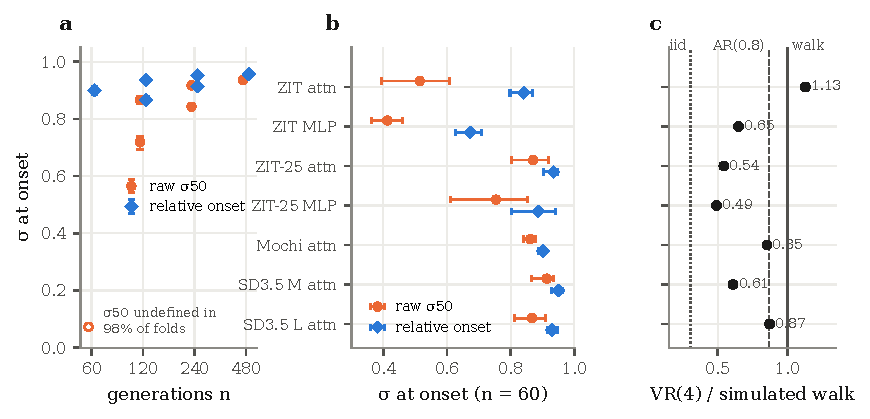
\includegraphics[width=\linewidth]{I-F10_estimators}
 \caption{Seed predictability rises gradually, and the raw $\sigma_{50}$ estimator depends on sample size. \textbf{(a)} Archive SD3.5\,M: raw $\sigma_{50}$ against the ceiling-free relative onset as the number of generations $n$ grows. $\sigma_{50}$ moves from undefined in 98\% of resamples at $n = 60$ to 0.94 at $n = 480$; the relative onset stays at 0.87--0.96. \textbf{(b)} At matched $n = 60$ (50 subsets; median and 5--95\% range), the relative onset is 0.84--0.95 in $\sigma$ in every channel except ZIT MLP (0.67). \textbf{(c)} VR(4) on the calibrated scale: observed divided by a simulated random walk, with AR(0.8) ($\approx 0.85$--$0.88$) and i.i.d.\ ($\approx 0.30$) references on this scale (their raw values are $0.72$ and $0.25$ against $0.82$ for the walk; Mode-II \S12). Seed deviations lie at 0.49--0.87 of walk, mostly below the AR(0.8) reference (only Mochi and SD3.5\,L reach it), except ZIT attention (1.13), a value its 8-state grid produces (subsampling other channels to 8 states gives 1.13--1.35; Round 8). $\sigma_{50}$ values are not compared across different $n$, and no commitment step is implied.}
 \label{fig:seed}
\end{figure}

\paragraph{Distilled checkpoints are less seed-sensitive (post hoc).} The seed share of the depth profile (within-prompt variance over total variance, standardised features) is much larger in both Base checkpoints than in their distilled students at matched $\sigma$ (post hoc): Z-Image attention $0.11$--$0.14$ against $0.05$--$0.08$, MLP $0.23$--$0.46$ against $0.08$--$0.17$; ACE-Step $0.51$--$0.79$ against $0.03$--$0.19$; prompt-bootstrap intervals exclude zero at every $\sigma$. The gap is already present at $\sigma=1$, before any guidance history. The Base captures ran at CFG 4 and the students at CFG 1, but guidance works against this contrast: in SD3.5 Medium, CFG 4.5 halves the seed share of the conditional branch relative to CFG 1 ($0.23$--$0.28$ against $0.30$--$0.66$ after step 0; Round 15, preregistered, R15-2). Reduced seed sensitivity is a candidate internal signature of reduced sample diversity in the distilled students, not evidence of commitment; an output-level diversity measure and a Base/Turbo capture at matched guidance and seed count are the clean tests.

%=====================================================================
\section{An intervention hierarchy}\label{sec:interventions}

Different interventions move the geometry by very different amounts (Fig.~\ref{fig:interventions}).
\begin{itemize}
 \item \textbf{Fixed weights, changed inference.} Mochi with CFG 1.0 versus 4.5 keeps registered shape at $0.9965$ (also a 100- versus 30-step comparison). SD3.5 Medium at $512$, $768$ and $1024$ pixels on the clean Round 4 captures (CFG 4.5, explicit branches, 30 prompts) moves the main $\beta$ crossing only within $g^*=0.074$--$0.085$, and the pooled Round 3 captures at the same three resolutions all show the depth sign sequence $+,-,+,-$ (24-bin estimator of the review rounds); the conditional plateau onset moves from $0.72$ to $0.76$ to $0.81$, and onto $0.84$, $0.81$, $0.81$ on the resolution-corrected clock. Resolution therefore shifts the operating point in $\sigma$ rather than the organisation. (A legacy single-prompt suite gives shape $0.989$--$0.996$ across resolutions; Supplement~\ref{app:legacy}.) Z-Image Turbo at 8 versus 25 steps, CFG 1 versus 4 and cond-only versus pooled capture keeps shape at $0.973$ (attention) and its tangent at $0.94$/$0.97$; at matched capture, $0.996$ and $0.99$ (Round 12 Z3).
 \item \textbf{Fixed architecture, targeted weight edit.} Abliteration of Mistral 7B \citep{arditi2024refusal} edits the weights to remove one direction, and keeps shape at $0.99977$; at prefill the median $|\Delta\log g|$ is $0.0013$, layers 0--5 are bit-identical, and the final layer moves four times more than any other. The depth tangent is kept: at prefill the tangent cosine between the two models is $0.9998$ (prompt bootstrap $0.99976$--$0.99983$; Round 9 R9-B3). After the prompt the sampled texts diverge at a median of generated token 7, so only the prefill is a clean comparison.
 \item \textbf{Scaling.} Qwen2.5 1.5B, 3B and 7B keep broad state resemblance (registered correlation $0.45$--$0.63$) but not depth derivatives: at matched $n$ the derivative correlation is $+0.63$ for 1.5B$\leftrightarrow$3B (prompt bootstrap $0.61$--$0.65$, above a layer-permutation null whose 95th percentile is $0.38$), $-0.12$ for 1.5B$\leftrightarrow$7B ($-0.16$ to $-0.08$) and $-0.06$ for 3B$\leftrightarrow$7B ($-0.10$ to $-0.01$), and in all three pairs it rises monotonically with context length (preregistered, Round 9 R9-B2). Scaling can therefore keep part of the local derivative, but not reliably. Why the 7B model breaks with the other two is untested; depth does not explain it, since the 1.5B and 7B models both have 28 layers. The three sizes share one chat-template regime (identical prefill lengths for all 24 prompts). SD3.5 Medium$\leftrightarrow$Large fails registration throughout, with shape $0.32$ and tangent $-0.25$; the pair differs in depth (24 and 38 layers), and its tangent changes sign under small depth shifts (\S\ref{sec:depthcal}).
 \item \textbf{Lineage (Base and a distilled or sibling checkpoint).} Z-Image Base and Turbo, siblings within one family, Turbo distilled from an unreleased SFT model (\S\ref{sec:intro}), keep registered shape at $0.85$ (attention) and $0.80$ (MLP) and the depth tangent at $0.55$/$0.77$ on the native grid ($0.71$/$0.72$ on the preregistered 24-point grid, Round 12). ACE-Step Base and its distilled turbo checkpoint keep shape at $0.71$/$0.61$ and the tangent at $0.85$/$0.57$ (Round 14). The shape $0.97$--$0.99$, tangents $0.94$--$0.99$ and MLP eigenmode closure ($p=0.002$) measured on the archive belong to the same Turbo weights under changed inference (first bullet), not to this lineage.
 \item \textbf{Capture functional.} With the trajectory held fixed, pooling the branches shifts $\log g$ by $+0.04$ to $+0.09$ (\S\ref{sec:instrument}).
\end{itemize}
Guidance, resolution, step count, a targeted weight edit and capture move the operating point or deform shape slightly. Distillation deforms shape more and keeps an intermediate share of the depth tangent, in two model families. Scaling preserves coarse resemblance but not local dynamics. Whether the retained tangent comes from the distillation objective or from shared pretraining is not separable here.

\begin{figure}[t]
 \centering
 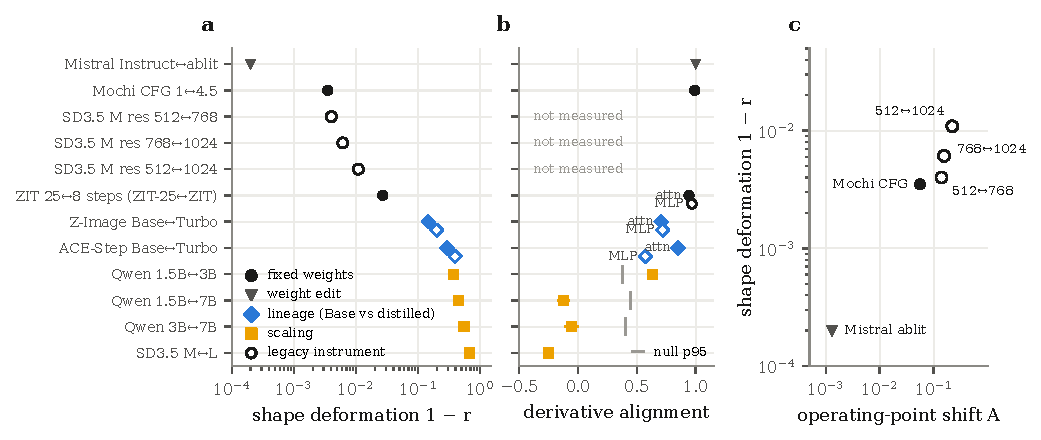
\includegraphics[width=\linewidth]{I-F11_intervention_hierarchy}
 \caption{Depth-shape deformation orders interventions. \textbf{(a)} Normalized shape deformation $1-r$: fixed-weight comparisons (Mochi CFG\,1$\leftrightarrow$4.5 0.9965; SD3.5\,M resolution pairs) and the targeted weight edit (Mistral Instruct$\leftrightarrow$abliterated 0.9998): $2\times10^{-4}$ to $1.1\times10^{-2}$; the same Turbo weights at 25 vs 8 steps, CFG 4 vs 1, pooled vs cond-only (\TT{}$\leftrightarrow$ZIT): 0.027; distillation lineages: Z-Image Base$\leftrightarrow$Turbo 0.15/0.20 and ACE-Step Base$\leftrightarrow$Turbo 0.29/0.39 (attn/MLP); capacity scaling: Qwen2.5 sizes 0.37--0.55 (one minus the registered correlations $0.45$--$0.63$) and SD3.5\,M$\leftrightarrow$L 0.68 (shape $0.32$, \S\ref{sec:interventions}). The SD3.5 resolution rows (open markers) use one prompt at CFG\,1 with the legacy instrument. The Mochi CFG comparison is also 30 vs 100 steps. \textbf{(b)} Local-dynamics alignment where it was measured: matched-$\sigma$ tangent cosine for diffusion (Mochi CFG 0.99; \TT{}$\leftrightarrow$ZIT 0.94/0.97 attn/MLP, same weights; Z-Image Base$\leftrightarrow$Turbo 0.71/0.72 on 24 points (0.55/0.77 native) and ACE-Step Base$\leftrightarrow$Turbo 0.85/0.57, lineage; SD3.5\,M$\leftrightarrow$L $-0.25$), the prefill depth-tangent cosine for the Mistral abliteration (0.9998, Round 9), and median depth-derivative $r$ at matched context length for Qwen (0.63, $-0.12$, $-0.06$). The Qwen prompt-bootstrap 5--95\% intervals are narrower than the markers; gray ticks mark each pair's layer-permutation null 95th percentile (0.38--0.45), which only 1.5B$\leftrightarrow$3B exceeds. \textbf{(c)} For the fixed-weight comparisons and the weight edit, shape deformation against the absolute operating-point shift $A$ (0.001--0.22): the root-mean-square difference between the two conditions of the population-mean absolute (unstandardised) statistics $(\log g,\log\gap,H)$ over matched (layer, state) cells, whereas shape is computed after standardising each profile across depth. These changes move the operating point while leaving the shape almost unchanged.}
 \label{fig:interventions}
\end{figure}

%=====================================================================
\section{Falsification results that define the claim boundary}\label{sec:falsification}

The following results were proposed during the project and did not survive. They are part of the empirical result and fix the claim boundary of this paper; Table~\ref{tab:retired} lists them, and Supplement~\ref{supp:fals} gives each with its numbers and Fig.~\ref{fig:sync}.

\begin{table}[htbp]
\centering\small
\caption{Retired claims. Each was proposed during the project and did not survive the test named. The last column says what the paper would have concluded had the claim held.}
\label{tab:retired}
\footnotesize
\begin{tabularx}{\linewidth}{@{}>{\raggedright\arraybackslash}p{0.2\linewidth}L>{\raggedright\arraybackslash}p{0.1\linewidth}>{\raggedright\arraybackslash}p{0.25\linewidth}@{}}
\toprule
Claim & What retired it & Status & If it had held\\
\midrule
Mid-run synchronisation peak ($R=0.81$--$0.93$) & a straight-line surrogate peaks as high in 7 of 7 channels; the monotone-warp null is not beaten in 4 of 7 (prereg.\ S5) & not an event & a shared mid-run event in every model\\
Universal semantic clock & semantic Fisher peak at $0.14$--$0.69$ of normalised time & retired & one semantic clock across models\\
Universal curvature, susceptibility, seed collapse & peaks at endpoints or mutually incompatible; seed share model-dependent; the $\sigma\approx1$ elevation coincides with pooled capture & retired & universal critical points of sampling\\
Raw $\sigma_{50}$ seed-onset contrast & $\sigma_{50}$ tracks sample size ($0.72$--$0.94$ over $n=120$--$480$) & replaced by relative onset & guidance or regime moves seed commitment\\
Autoregressive $\beta$ ladder (Qwen2.5-7B) & the statistic is a running statistic over context; i.i.d.\ rows with no model reproduce $|\rho|=1$ (R9-B1) & demoted & a size ladder in language models\\
Architecture ordering of scalar curves & capture regime and projection; both ``Z-Image'' campaigns are Turbo & retired & architectures ranked by scalar curves\\
Lineage read from an archive label ($0.94$--$0.99$) & identity gate: both campaigns are Turbo; real sibling lineage $0.71$/$0.72$ (24 points; $0.55$/$0.77$ native) & replaced & lineage nearly identical to same weights\\
Z-Image Base depth sequence and clock-axis contraction & real Base has one depth crossing and no contraction & Turbo, caption rows & a Base-model depth and clock signature\\
Depth sequence specific to image data & absent in ACE-Step Base and in real Z-Image Base & retired & a modality marker\\
Pooled-cloud fixed points & some crossings null-generic under marginal and mean-field surrogates & retired & fixed points of the pooled dynamics\\
Rotation index $\varphi$ & raw $-1/2$ is the differencing null (Mode-II); adds no held-out information & retired & a rotation of the trajectory\\
Middle tier specific to distillation & SD3 M$\leftrightarrow$SD3.5 M, not a distilled pair, $0.93$ (R17-2) & broad lineage & a distillation detector\\
MLP bottom tier & unrelated PixArt-$\Sigma$$\leftrightarrow$Cosmos MLP $0.69$, in the lineage range (R17-1) & attention only & tiers in both submodules\\
\bottomrule
\end{tabularx}
\end{table}


%=====================================================================
\section{An out-of-family check: a convolutional U-Net}\label{sec:unet}

Every model in the archive is a transformer denoiser trained on natural images. To see which results depend on the transformer family, we captured Stable Diffusion~1.5 \citep{rombach2022high}, a latent diffusion model whose denoiser is a convolutional U-Net \citep{ronneberger2015unet} with 16 transformer blocks embedded at four resolutions. Hooks read the self-attention output and the MLP output of each block. Width and token count change with the level: $(N,D)=(4096,320)$, $(1024,640)$, $(256,1280)$ and $(64,1280)$ in the middle block at $512$ pixels. The run used 476 generations on 119 of the archive prompts (about four seeds each), 50 steps, CFG 7.5 and explicit per-branch rows; all numbers below use the conditional branch, and the unconditional branch gives the same verdicts. Three predictions were frozen before the capture existed (SHA-256 prefix \texttt{efa613eb}, 2026-10-08 15:27 UTC), and the operational choices they left open were frozen before scoring (\texttt{7a3b852f}, 21:46 UTC). Every other number in this section is post hoc.

\paragraph{Preregistered.} Because $D$ and $N$ change across blocks, each block is compared with the value $g_{\rm MP}(N,D)$ that a white Gaussian matrix of the same shape gives \citep{marchenko1967distribution}.
\begin{itemize}
 \item \emph{Anisotropy (C1), tested and not supported.} The prediction was $g/g_{\rm MP}<0.10$ in at least $95\%$ of (step, block) cells, as in the archive transformers, whose median ratios are $0.018$--$0.071$ for attention and $0.0014$--$0.0019$ for the Z-Image MLP (a caption-row statistic, Table~\ref{tab:captionmap}). In SD1.5 the median ratio is $0.077$ for attention, with $31\%$ of cells at or above $0.10$, and $0.26$ for the MLP, with $95\%$ of cells above. The U-Net MLP is about a hundred times closer to isotropy than the Z-Image MLP. The image-token MLPs of PixArt-$\Sigma$ and Cosmos sit between them (medians $0.114$ and $0.058$), and all four Round 17 models fail the $95\%$ rule in attention as well (medians $0.057$--$0.074$, $10$--$55\%$ of cells at or above $0.10$; post hoc, RC35), so strong anisotropy in the sense of C1 is a property of some transformers, not of transformers as such. Strong anisotropy of the uncentred second moment is therefore not a fixed property of denoisers. We do not know the cause. Candidates are the few extreme activation channels that dominate uncentred transformer spectra \citep{sun2024massive}, the U-Net's group normalisation and convolutional mixing ahead of each transformer block, and its small widths at the outer levels; none is tested.
 \item \emph{Depth step is not a function of $g$ (C2), confirmed.} With the layer-step definition used throughout, $\beta_{\rm layer}=g_{\ell+1}-g_\ell$, a block effect adds a held-out $\Delta R^2$ of $0.46$ (attention) and $0.61$ (MLP) to a spline in $g$ (5-fold cross-validation grouped by prompt). The same test gives $0.49$--$0.65$ in every transformer channel. In this sense the depth step is non-autonomous in a U-Net as well (Mode-II).
 \item \emph{Depth beyond the level (C3), split.} On pairs of adjacent blocks within one level, block identity adds $\Delta R^2=0.22$ over the level in attention (prediction $\ge0.15$, confirmed) and $0.06$ in the MLP (tested, not supported). In the MLP, the level's width and token count account for almost all of what depth explains.
\end{itemize}

\paragraph{Post hoc.} Each analysis uses the archive method unchanged.
\begin{itemize}
 \item \emph{Backbone.} PC1 is $0.90$ (attention) and $0.62$ (MLP), with effective rank $1.46$ and $2.24$. Both beat all 999 depth-shift nulls (null means $0.22$ and $0.19$; $p=0.001$). The same implementation gives $0.90$ and $0.68$ on SD3.5 Medium and the 25-step Turbo MLP.
 \item \emph{The spectral triple is two-dimensional.} The first two principal components of the triple $(H,\log Dg,\log\gap)$, with both entropies divided by $\log D$, hold $0.995$ and $0.987$ of the variance, against $0.980$--$0.994$ in the transformers.
 \item \emph{Content geometry.} The ordered depth profile at the first state decodes the ten domains at $0.38$ (attention) and $0.42$ (MLP). This beats every depth scramble (maximum $0.17$ and $0.19$; $p=0.01$) and the layer mean ($0.19$, $0.18$), but only matches the TF-IDF decoder on the prompt text ($0.40$); the transformers exceed it (Table~\ref{tab:decode}). Prompt-relational geometry is shared with every transformer (Fig.~\ref{fig:unet}c): on the 116 prompts common to all six models, Mantel $\rho$ between SD1.5 attention and the five transformers is $0.11$--$0.35$ (every $p=0.0005$), the lower part of the $0.14$--$0.43$ range of unrelated transformer pairs on the same prompts.
 \item \emph{Plateau onset.} SD1.5 uses a variance-preserving $\varepsilon$-prediction schedule. Mapped to the rectified-flow clock at equal signal-to-noise ratio, $t=\sigma/(1+\sigma)$, the onset is $0.58$ (attention) and $0.67$ (MLP), below the archive's $0.78$--$0.87$ at $1024$ pixels. With the SD3 resolution shift for $512$ pixels it is $0.73$ and $0.80$, against $0.84$ for SD3.5 Medium at $512$ pixels on the same correction. The schedule starts at $t=0.94$, so the transient at $\sigma\approx1$ is truncated, and this comparison depends on the clock mapping.
 \item \emph{Prompt share.} Within a sampling state, prompt identity explains $0.56$--$0.67$ of the variance (ANOVA share), inside the archive's $0.36$--$0.95$.
 \item \emph{Clock-axis envelopes.} The layer-mean $g$ of both submodules rises over the whole schedule ($+,+,+$ in every bootstrap, on all three clock mappings; Fig.~\ref{fig:sigma}). The transformers' attention late fall and the Z-Image MLP contraction are both absent. This analysis was defined in writing before it was run (22:45 UTC, \texttt{6251b69f}) but after the data were seen, so it is post hoc.
\end{itemize}
The layer-axis sign structure of \S\ref{sec:topology} was not tested. Pooling $\beta$ across U-Net levels with different $D$ and $N$ is not meaningful, and the preregistration excluded it for that reason.

\begin{figure}[t]
 \centering
 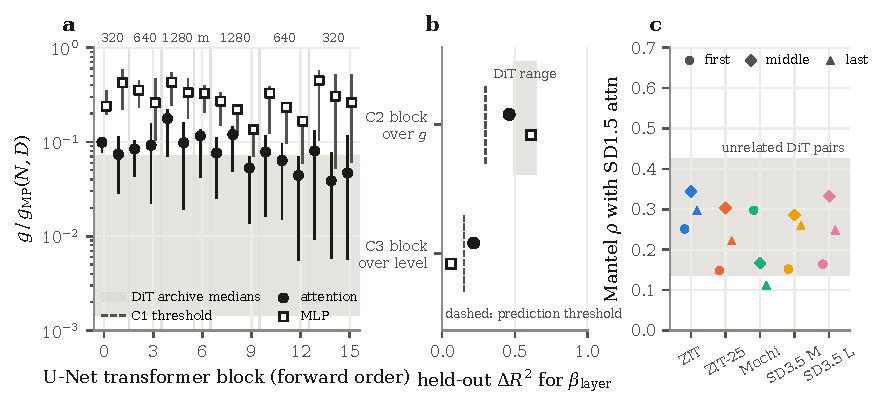
\includegraphics[width=\linewidth]{I-F13_unet}
 \caption{Out-of-family check on the SD1.5 U-Net (conditional branch). \textbf{(a)} Preregistered C1: per-block $g/g_{\rm MP}(N,D)$, median over 476 generations (markers) and range over 50 steps (bars), with the block width above. The transformer archive's median ratios lie in the grey band. The prediction ($<0.10$ in $\ge95\%$ of cells) fails: $31\%$ of attention cells and $95\%$ of MLP cells reach $0.10$. \textbf{(b)} Preregistered C2 and C3: held-out $\Delta R^2$ for $\beta_{\rm layer}$ of a block effect over a spline in $g$ (C2; transformer range in grey) and over the U-Net level on within-level pairs (C3). Dashed: prediction thresholds. \textbf{(c)} Post hoc: Mantel $\rho$ between the prompt-dissimilarity matrices of SD1.5 attention and each transformer on 116 shared prompts at the first, middle and last step (every $p=0.0005$); grey: unrelated transformer pairs on the same prompts.}
 \label{fig:unet}
\end{figure}

What carries over to the U-Net is a low-dimensional backbone, a two-dimensional triple, a depth step that is not a function of $g$, content-bearing depth order and prompt-relational geometry shared with transformers. What does not carry over is the degree of anisotropy, most strongly in the MLP. Domain decoding is weaker, the plateau onset is later on the matched clock under the $2\times$ rule (not under the $1.5\times$ or $3\times$ rule), and the clock-axis envelopes rise monotonically. This is one U-Net trained on natural images, so its results are existence statements: they show that a property can occur, or fail to occur, outside the transformer family, not how often. It separates the transformer block from the rest of the setup, but not the data or the objective.

%=====================================================================
\section{An out-of-modality check: an audio flow transformer, distilled and undistilled}\label{sec:ace}

The U-Net changes the block architecture but keeps natural-image data. To change the data modality instead, we captured ACE-Step~1.5 \citep{gong2026acestep15}, a music-generation flow transformer with 24 layers and width $D=2048$ whose sampled latent is a 180-second audio clip ($N=2250$ tokens, so $N\ge D$ as in the image captures). Its even layers use sliding-window self-attention over 128 tokens and its odd layers full attention. Hooks read the self-attention and MLP outputs of every layer. The run used the six-step distilled turbo checkpoint at CFG 1 (conditional branch only), 120 generations on 29 instrumental prompts in ten genre domains, mostly four random seeds per prompt. Ten predictions (B1--B10) were frozen before the capture existed, in the same preregistration as the U-Net arm (\texttt{efa613eb}, 2026-10-08 15:27 UTC). The scoring plan, which records how the capture departed from the protocol (turbo checkpoint, six steps, 29 of the 30 prompts) and fixes the operational rules, was frozen before scoring (\texttt{7fa54aab}, 2026-10-09 06:36 UTC). Every number not tied to B1--B10 is post hoc. The instrument gate B1 passed: 24 layers $\times$ two submodules on every step, $N=2250$, $D=2048$.

\paragraph{Preregistered results.}
\begin{itemize}
 \item \emph{Anisotropy (B2), tested and not supported.} The prediction was $g/g_{\rm MP}<0.10$ in at least $95\%$ of (step, layer) cells, with $g_{\rm MP}=0.75$ the isotropic value at this $(N,D)$. The median ratio is $0.15$ for attention and $0.30$ for the MLP, and $72\%$ and $95\%$ of cells reach $0.10$ (Fig.~\ref{fig:ace}a). As in the U-Net, the MLP sits far closer to isotropy than in the image transformers.
 \item \emph{The triple is two-dimensional (B3), tested and not supported.} The first two principal components of $(H/\ln D, \ln(gD)/\ln D, \ln\gap)$ carry $0.988$ of the variance in attention but $0.976$ in the MLP, just below the threshold of $0.98$ (images: $0.980$--$0.994$).
 \item \emph{Depth step is not a function of $g$ (B4), confirmed.} A layer effect adds a held-out $\Delta R^2$ of $0.60$ (attention) and $0.77$ (MLP) to a spline in $g$, against $0.49$--$0.65$ in the image channels.
 \item \emph{Layer parity (B5), confirmed.} Even layers have higher $\log g$ than odd layers in every (generation, step) cell (median difference $0.58$ in attention; the MLP shows the same sign, $0.12$, descriptively). The depth profile is a zig-zag that follows the attention window (Fig.~\ref{fig:ace}a).
 \item \emph{Layer-axis recurrence (B6), tested and not supported.} The analyzer's binned $\beta_{\rm layer}(g)$ for attention has a single crossing ($+,-$ at $g^{*}=0.090$), not the three of the image archive, in 99 of 100 prompt bootstraps (Fig.~\ref{fig:ace}b). The even-layer subsequence alone gives three crossings and the odd-layer subsequence one (descriptive). The crossing-slope prediction B7 depended on B6 and was not run.
 \item \emph{Plateau onset (B8), confirmed.} The onset lies at $\sigma=0.90$ (attention) and $0.80$ (MLP), inside the window $[0.73,0.92]$. With six steps only one interval lies below $\sigma=0.6$, so the plateau speed that defines the onset rests on that interval; with a window $0.19$ wide, the test was weakly identified.
 \item \emph{No susceptibility peak (B9), confirmed.} The seed variance of $\operatorname{logit} g$ has its maximum at the interior step $\sigma=0.60$ in every bootstrap, but it does not beat the last step by two bootstrap standard errors, so no peak passes the preregistered rule (Fig.~\ref{fig:ace}c). The curve is not flat; the rule, not the shape, decides this verdict.
 \item \emph{Prompt share rises first (B10), tested and not supported.} The prompt share of geometry variance is already $0.96$ (attention) and $0.94$ (MLP) at $\sigma=1$, dips to $0.86$ and $0.82$ at $\sigma=0.60$ and recovers at the last step, so its steepest rise is in the last interval, not the first.
\end{itemize}

\paragraph{Post hoc results.} The temporal backbone recurs: PC1 $0.78$ and $0.56$, effective rank $2.10$ and $2.73$, against depth-shift null ranks of $3.9$ and $4.1$ ($p=0.001$ and $0.011$; with six states the rank is at most five, Fig.~\ref{fig:backbone}). The clock-axis envelopes of both submodules peak at $\sigma=1$ and follow $-,+,-$ in every bootstrap (\S\ref{sec:topology}, Fig.~\ref{fig:sigma}). In the analyzer replay (Table~\ref{tab:beta}) attention has a single crossing at all six steps and in every generation bootstrap, and both surrogates reproduce it; the MLP has three crossings at 2 of 6 steps and in $5\%$ of generation bootstraps. Domain decoding is not informative, because 29 prompts give only two or three per domain and even a decoder on the prompt text is at chance (Table~\ref{tab:decode}). Prompt-relational geometry and depth tangents were not compared with the image models, which saw different prompts.

\begin{figure}[t]
 \centering
 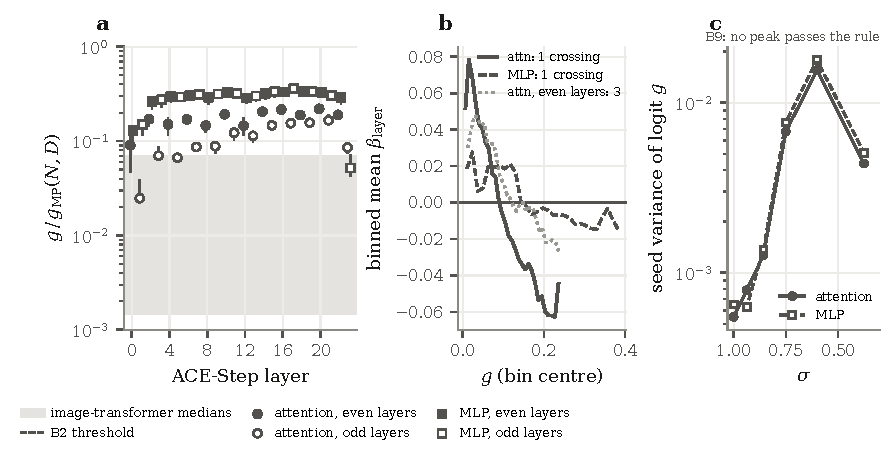
\includegraphics[width=\linewidth]{I-F14_ace}
 \caption{Out-of-modality check on the audio flow transformer ACE-Step~1.5 (turbo, 6 steps, cond-only, 120 generations, 29 prompts; the Base checkpoint is in Fig.~\ref{fig:tiers}). \textbf{(a)} Preregistered B2 and B5: per-layer $g/g_{\rm MP}$ ($g_{\rm MP}=0.75$), median over generations (markers) and range over steps (bars); even layers (sliding-window attention) filled, odd layers (full attention) open. Grey band: image-transformer median ratios. B2 fails ($72\%$ of attention and $95\%$ of MLP cells reach $0.10$); the even--odd zig-zag holds in every cell (B5). \textbf{(b)} Preregistered B6: the analyzer's binned $\beta_{\rm layer}(g)$, all steps pooled. Attention and MLP each cross zero once, not three times; the even-layer subsequence alone crosses three times (descriptive). \textbf{(c)} Preregistered B9: seed variance of $\operatorname{logit} g$ along $\sigma$. The interior maximum at $\sigma=0.60$ does not clear the last step by two bootstrap SE, so no peak passes the rule.}
 \label{fig:ace}
\end{figure}

\subsection{The undistilled checkpoint: ACE-Step~1.5 Base (Round 14)}
The turbo arm left modality confounded with distillation and step count. ACE-Step~1.5 Base was therefore captured on the same 30-prompt protocol: 50 steps, CFG 4 with explicit per-branch rows, two seeds per prompt (60 generations, all complete), 180 seconds, run on two GPUs whose files were joined by prompt hash and seed. Two tests had been frozen for it in Round 12 (\texttt{ad06a1bb}, 2026-10-18): the lineage tangent against the turbo checkpoint (R12-6) and a decision rule for the depth sign sequence (R12-7: three crossings modal in at least $50\%$ of bootstraps would attribute the turbo result to distillation, one crossing modal to modality). Before any statistic other than the identity gate was computed, a second preregistration (\texttt{dc997f6d}, 2026-11-05) fixed the operational choices, replayed B1--B10 unchanged on the Base conditional branch, and added six predictions. The identity gate passes: the step-0 depth profile correlates with the turbo checkpoint at only $0.34$ (attention) and $0.70$ (MLP), against $\ge0.92$ for turbo against itself. The two GPU halves agree (tangent $0.992$/$0.972$, field correlation $0.998$; R14-1), so they are pooled.

\paragraph{Preregistered results.}
\begin{itemize}
 \item \emph{Lineage (R12-6), supported.} Base$\leftrightarrow$turbo tangent $0.850$ (attention) and $0.572$ (MLP), against layer-permutation nulls of $0.316$ and $0.242$; both are at least $0.30$ above the null and below $0.95$ (\S\ref{sec:similarity}, Table~\ref{tab:tiers}). The MLP margin is narrow ($0.03$ above its bound).
 \item \emph{Depth sign sequence (R12-7).} Base attention has a single crossing in 100 of 100 prompt bootstraps. By the frozen rule, the single crossing of the turbo checkpoint is attributed to modality, not to distillation.
 \item \emph{B1--B10 replayed.} B1 passes, B5 (even layers above odd in every cell) and B8 (onset $\sigma=0.79$ and $0.85$) hold, and B2, B3 and B6 fail as in turbo (median $g/g_{\rm MP}$ $0.095$ and $0.276$, with $48\%$ and $89\%$ of cells at or above $0.10$; PC1+PC2 $0.9875$ and $0.9794$). Three verdicts differ from turbo. B4 fails in attention: a layer effect adds only $\Delta R^2=0.254$ to a spline in $g$ ($0.689\to0.943$), because $g$ alone already predicts the attention layer step well; the MLP adds $0.671$. B9 fails: the seed variance of $\operatorname{logit} g$ has an interior attention peak at the sixth step ($\sigma=0.957$), stable in $92\%$ of bootstraps and above both ends by more than two standard errors, inside the early transient. B10 holds: prompt share rises most in the first interval ($0.34\to0.46$ and $0.22\to0.41$).
 \item \emph{New predictions.} Conditional and unconditional branches share the fingerprint (tangent $0.997$/$0.964$; R14-3), the last MLP layer collapses ($\log g$ at layer 23 is $2.30$ below the median of layers 12--22, turbo $1.87$; R14-4), and the parity sign carries over (even above odd in $100\%$ of attention cells; R14-5). Two predictions fail: Base is not uniformly more concentrated than turbo (lower $g$ in 14 of 24 attention and 10 of 24 MLP layers; R14-2), and prompts do not dominate the final state (corrected prompt share $0.48$ and $0.52$ at the last step, against a threshold of $0.70$, fixed in the Round 14 preregistration below the turbo values of $0.82$--$0.96$; R14-6).
\end{itemize}

\paragraph{Post hoc.} The backbone recurs (PC1 $0.81$/$0.71$, rank $1.87$/$2.27$, $p=0.001$), the MLP depth axis has two crossings ($-,+,-$ in every bootstrap), and the clock-axis fits are $-,+,+$ (attention) and $+,+,-$ (MLP). Against the image models, ACE-Step Base tangents lie in the unrelated range ($-0.11$ to $0.27$ in attention, $0.13$ to $0.20$ in MLP).

\subsection{The release setting and a step panel (Round 16)}\label{sec:ace16}
The turbo arm ran at 6 steps, the default of the ComfyUI workflow, where the release recommends 8. Round 16 (\texttt{a3b59c92}, frozen 2026-11-06 15:05 UTC, before the capture) recaptured turbo on the Base prompts and seeds at CFG 1 and shift 3: 8 steps with both seeds (60 generations, matching the Base run) and 1, 2, 3, 4, 5, 7, 9 and 10 steps with one seed (30 each); all 330 generations are complete. The identity gate places every arm with the turbo checkpoint and away from Base, though only in its undecided band, not its same-weights band (step-0 $r$ with the 6-step turbo capture $0.863$--$0.927$, inside $0.85$--$0.98$; with Base $0.169$--$0.383$).
\begin{itemize}
 \item \emph{Supported.} The lineage pair at 8 steps, $0.795$/$0.594$ (R16-2, R16-3; \S\ref{sec:similarity}); one layer-axis crossing at 8 steps, in 94 of 100 prompt bootstraps (R16-5); the last-layer MLP collapse at every step count from 2 to 10, growing slowly with the step count ($1.61$ to $1.83$; R16-6); and even layers above odd in every attention cell at every step count (R16-7).
 \item \emph{Refuted.} The 8-step and 6-step captures differ by more than the same-weights bar ($0.918$/$0.821$ against $0.94$; R16-1), a difference between capture sessions, not step counts (\S\ref{sec:similarity}); the 3-step MLP tangent against 8 steps is $0.906$, the one failure among 12 cells (R16-4); and at 8 steps with two fixed seeds per prompt the final-step prompt share is $0.692$ (attention) and $0.593$ (MLP), below $0.70$ (R16-8; the 6-step arm with four to eight random seeds per prompt gave $0.82$--$0.96$).
\end{itemize}
By the consequence fixed in advance, ACE-Step turbo results are stated at 8 steps where the 8-step arm can replace the 6-step one: the lineage values, the single crossing, the end collapse and the parity. B1--B10 and Fig.~\ref{fig:ace} remain the 6-step arm, where they were measured, and are a secondary arm. The prompt-share statement (B10 and R14-6) is scoped to the 6-step design.

\begin{figure}[!htbp]
 \centering
 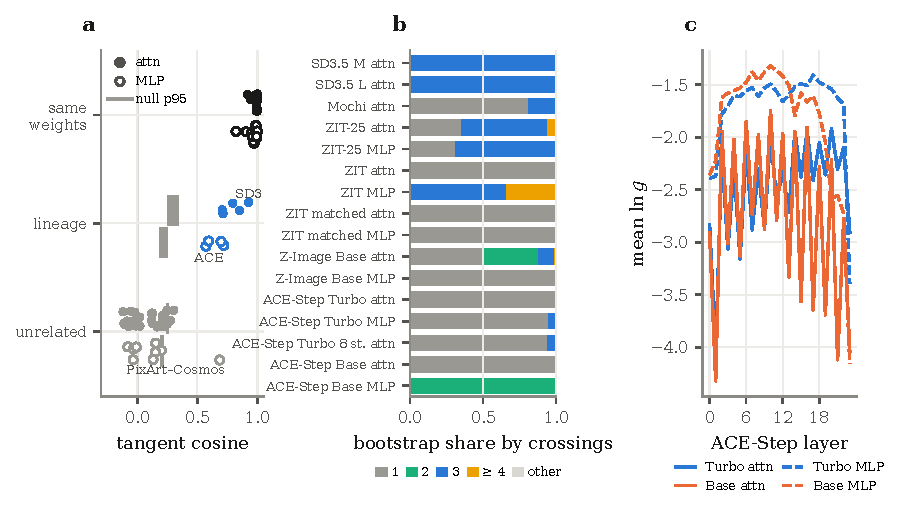
\includegraphics[width=\linewidth]{I-F15_tiers}
 \caption{Tiers, the crossing census and the two ACE-Step checkpoints (Rounds 12, 14, 16 and 17, preregistered values; panel (b) Base MLP and the unrelated ACE pairs in (a) are post hoc). \textbf{(a)} Matched-$\sigma$ tangent cosine by tier. Same weights under changed inference (25 vs 8 Turbo steps, matched Turbo rerun, conditional vs unconditional branch, GPU 0 vs 1, ACE-Step turbo at 3--10 steps, SD3.5 M recapture): 0.94--0.999 in attention; ACE-Step turbo across two capture sessions 0.92/0.82. Lineage now includes the same-vendor pair SD3 M$\leftrightarrow$SD3.5 M (``SD3'', 0.93, attention) and ACE-Step at 8 steps (0.80/0.59). Related pairs (depth-matched): Z-Image Base$\leftrightarrow$Turbo siblings 0.71/0.72 and 0.71/0.70 on 24 points (against Turbo and the matched Turbo rerun), ACE-Step Base$\leftrightarrow$Turbo 0.85/0.57 (attention filled, MLP open; gray ticks: layer-permutation null 95th percentiles, 0.20--0.32). Unrelated pairs (Z-Image vs SD3.5 and Mochi; ACE-Step vs every image model): $-0.12$ to $0.27$ over all of them (ACE-Step Base alone $-0.11$ to $0.27$, \S\ref{sec:ace}); the depth-matched image pair PixArt-$\Sigma$$\leftrightarrow$Cosmos (Round 17) is $0.30$ in attention and $0.69$ in MLP (``PixArt--Cosmos''). Only PixArt--Cosmos and the ACE-Step$\leftrightarrow$SD3.5 Medium pairs in the unrelated cloud are depth-matched; every other unrelated point is a cross-depth value and not a calibrated level (\S\ref{sec:depthcal}). Margins between the groups in (a), attention, depth-matched: same weights in a session over distillation lineage $0.15$--$0.29$ and over the successor $0.07$; distillation lineage over depth-matched unrelated pairs $0.40$--$0.96$ (\S\ref{sec:tierstatus}). Values are the preregistered 24-point ones; on the native grid the Z-Image siblings read $0.55$/$0.77$ on all rows (Table~\ref{tab:tiers}). (b) adds ACE-Step turbo attention at 8 steps (R16-5). \textbf{(b)} Share of 100 prompt bootstraps with 1, 2, 3 or $\geq4$ layer-axis crossings of the analyzer's $\beta_{\text{layer}}$. Three crossings are modal only in SD3.5 M/L attention, the 25-step Turbo campaign and ZIT MLP; the real Z-Image Base, the matched Turbo rerun, and both ACE-Step checkpoints are not $+,-,+,-$. The SD3.5 and Mochi rows record only the 1, 3 and $\geq5$ shares (Round 6). \textbf{(c)} Mean $\ln g$ (natural logarithm) by layer, ACE-Step Base at the Turbo $\sigma$s (R14-2): Base is lower in only 14 (attention) and 10 (MLP) of 24 layers, and both checkpoints share the even/odd alternation and the last-layer MLP drop.}
 \label{fig:tiers}
\end{figure}

\subsection{What the audio arms show}
What carries over to audio, in both checkpoints, is the low-dimensional backbone, the layer parity set by the attention window and a plateau onset inside the image range. What does not carry over is the strong anisotropy and the depth sign sequence $+,-,+,-$. The two checkpoints disagree on whether the depth step is a function of $g$ in attention, on a susceptibility peak and on the early rise of prompt share; each of these is stated per checkpoint. The depth sign sequence is absent from undistilled audio too, so its absence is not a distillation effect, as the frozen rule records. It does not follow that the sequence is a property of image data: the real Z-Image Base, an undistilled image model, lacks it in its conditional branch as well (Table~\ref{tab:beta}), and the same Turbo weights show or lose it with the capture settings. These are existence statements from one audio model in two checkpoints. The sequence is therefore not ``image- and video-specific''; it is specific to models and capture settings (SD3.5, Mochi, Z-Image Turbo at 25 steps), and in SD3.5 Medium it depends on the uncentred mean direction. Z-Image Turbo, distilled and few-step, keeps image-transformer anisotropy in its MLP (median $g/g_{\rm MP}$ $0.0014$--$0.0019$ in the Z-Image MLPs, against $0.28$--$0.30$ for both ACE-Step MLPs), so neither distillation nor step count produces the near-isotropy of the audio MLPs.

\FloatBarrier
%=====================================================================
\section{Synthesis}\label{sec:synthesis}
\begin{enumerate}
 \item Coarse organisation recurs across architectures and modalities: a low-dimensional backbone and an early transient followed by a $\sigma$-plateau. The depth sign sequence $+,-,+,-$ does not belong to this list: it appears in SD3.5, Mochi and Z-Image Turbo at some noise level, beats a mean-field surrogate at 6--12 single steps in SD3.5 Medium, SD3.5 Large, Mochi and 25-step Turbo attention, is null-generic pooled in SD3.5 Large, vanishes on centring in SD3.5 Medium, and is absent from the real Z-Image Base conditional branch and from both ACE-Step checkpoints. Evidence for a recurrent depth topology would need the same sign sequence at matched $\sigma$ beyond the surrogate nulls, stable under centring and row selection, in models that do not share weights; the data show it in some channels at some steps and rule out one sequence common to all models.
 \item \emph{(PA.)} A weak but reliable component of prompt-relational geometry is shared ($\rho=0.13$--$0.43$ between unrelated models), beyond theme and text, and strongest for the same weights; cross-model orderings of it hold at each model's recommended operating point, and RSA moves with that point (the same SD3.5 Medium weights give $0.75$ at CFG 1 and $0.38$ pooled at CFG 4.5), so the claim is about model and operating point together. It is shared between models with different text encoders (Z-Image's Qwen3 encoder against Mochi's T5: $0.39$, above SD3.5 Medium against Large, which share all three encoders, $0.31$). It does not replicate between the two audio checkpoints, a test with little power (RC23A).
 \item \emph{(Measured: LA, OOS; the finer ordering is a hypothesis; the qualifiers are stated once, in \S\ref{sec:tierstatus}.)} Among the depth-matched pairs measured, attention depth dynamics separate the related pairs from the two unrelated pair types on the native grid and on grids of 24 points or finer, and within the related pairs suggest an ordering: same weights ($0.98$--$0.999$ in a session; $0.92$--$1.00$ across sessions), a same-vendor successor ($0.93$) level with a documented teacher--student pair (SD3.5 Large, $0.90$), the ACE-Step Base--turbo pairs ($0.80$--$0.85$), and unrelated pairs ($-0.17$ to $0.20$). A preregistered activation-CKA baseline on nine of the models does not reproduce this separation (\S\ref{sec:cka}). The Z-Image siblings, derived separately within one family, sit between distillation and unrelated pairs on all rows ($0.55$; $0.71$ on 24 points) and level with the successor on image rows ($0.91$): separately derived models of one family keep a measurable common depth dynamics. In MLP the tiers do not hold ($0.57$ for an unrelated pair; $0.69$ on 24 points). The one cell that approaches same weights, Z-Image attention on image rows, suggests a hypothesis worth a direct test: at image positions attention may be dominated by spatial routing among latent patches, which output-matching distillation has no reason to change (\S\ref{sec:similarity}). In Z-Image, distillation changed the first and last layers and the size of the shared mean direction, and left the middle layers nearly unchanged.
 \item The same data therefore support a hierarchy of invariance, not one universal microscopic law.
 \item \emph{Confirmatory core.} If every analysis after Round 14 is treated as exploratory, what remains preregistered and replicated is: the attention tangent ordering (R12-1 to R12-6, R16-2, R17-1 to R17-4, R18-1, R18-2 and R18-4; Z-Image with disclosed lookahead, ACE-Step, the controls and the documented distillation pair out of sample), with the MLP bottom tier refuted (R17-1); the low-dimensional backbone (Round 1, replicated in Round 11); shared prompt-relational geometry (Round 6 S2, Round 8); and the relative onset replacing $\sigma_{50}$ (Round 6 S3). The identity gate is a post hoc audit tool, and the row-set, per-coordinate and seed-sensitivity results are hypotheses.
 \item In a convolutional U-Net the backbone, the non-autonomous depth step and shared prompt geometry recur, but the strong anisotropy of the archive transformer channels and their clock-axis envelope shapes do not (\S\ref{sec:unet}); four further transformers, captured for the tier controls, replicate the backbone, the two-component triple, decoding and prompt geometry and lack the strong anisotropy as well (post hoc, Supplement~\ref{supp:posthoc}).
 \item In an audio flow transformer, in both checkpoints, the backbone, the layer parity and the plateau onset recur, but the strong anisotropy and the depth sign sequence do not (\S\ref{sec:ace}). Its absence is not caused by distillation (Round 14), and since real Z-Image Base also lacks it, it is not caused by modality either.
 \item In Z-Image the uncentred MLP statistic is a caption-token statistic from layer 10 on, and the clock-axis contraction of Turbo MLP lives in those rows. Results for joint text--image sequences (Z-Image) and for image or visual streams (SD3.5, Mochi) should be read separately; MLP comparisons across them compare different row sets.
\end{enumerate}

\subsection{Practical use}\label{sec:practice}
Until the architecture control is run, the tangent's split is between the model families measured here, not between training relations in general, and with a false-positive bound of $45\%$ at best it is a screen to prompt a provenance check, not a decision rule. For someone capturing telemetry of their own models, the results reduce to six rules. (1) Name the capture functional of every number and never compare absolute $g$ across functionals: pooling raises $g$ by a known sign and a measured size (Mode-II \S3). (2) Capture the conditional branch, and, for joint text--image sequences, image rows; store centred statistics and a few leading singular values as well, so that later checks need no recapture. (3) Record the SHA-256 of every weight file; the hash is the provenance record. Run the first-state identity check as well, as an audit for runs whose metadata may be wrong: it costs one denoiser evaluation per prompt and in this record separates far-apart checkpoints (Base against distilled, unrelated models), but it reads close relatives as undecided ($0.93$--$0.94$ for SD3 against SD3.5 Medium), has no calibrated error rate, and has not been tested against a deliberate weight swap; it is an audit heuristic, superseded by the hash. (4) Compare two models' dynamics with the attention depth tangent only at equal depth, on the native grid (one point per hooked layer), against both a layer-permutation and a smoothness-preserving null, and with a same-weights reference captured in the same session. (5) Do not read envelope correlations as similarity: a shared trend sets their floor (Mode-II, trend dominance). (6) For seed predictability, report the relative onset at matched $n$, not $\sigma_{50}$. Why use telemetry when the weights are at hand? Weight-based comparison is stronger whenever two models' weights can be aligned, and should be preferred then. The tangent needs no alignment of parameters, so it compares models of different architecture and width (Mode-II, Lemma~9(ii)); it can be read from telemetry logged during ordinary generation, without storing activations; and for the adaptive-normalisation models here it is blind only to signed channel permutations (Mode-II, Corollary~10(c)), so it measures a near-functional similarity of depth dynamics rather than a parametric one. For distillation research the tangent is at most a screen, and only in the form of rule (4): attention, equal depth, read against a same-weights reference captured in the same session. No attention value currently separates the same weights from a close relative (ACE-Step across sessions $0.918$, the SD3 successor $0.926$), the MLP admits unrelated pairs ($0.57$--$0.69$; a same-vendor language-model pair $0.66$), and nothing here licenses a reading of distillation strength or of output quality (no quality labels, \S\ref{sec:limits}). A student that falls toward the unrelated range against its teacher is worth a closer look by other means; one that does not is not thereby shown to be close.

%=====================================================================
\section{Limitations and future tests}\label{sec:limits}
\begin{itemize}
 \item \textbf{Commitment.} A separatrix or commitment claim needs cloned continuations around candidate noise levels with scored final images (gate G3); recent work on semantic commitment in diffusion \citep{handke2026entropic,raya2023spontaneous} motivates it.
 \item \textbf{Autoregressive dynamics.} Per-token phases need context-invariant statistics (G4).
 \item \textbf{Output quality.} The archive has no stable output identifier or quality label, so no geometry$\to$quality statement is possible (D14).
 \item \textbf{Response.} Finite perturbations would turn the descriptive local maps into response or Jacobian measurements (G1).
 \item \textbf{Submodules.} Among the transformers, MLP hooks exist for Z-Image, PixArt-$\Sigma$ and Cosmos-Predict2 only; the clock-axis result needs them on Mochi and SD3.5, and the PixArt-$\Sigma$ and Cosmos MLPs do not show it (post hoc, Supplement~\ref{supp:posthoc}). The U-Net and the audio model have MLP hooks, and neither MLP shows the Z-Image clock-axis pattern (post hoc, \S\ref{sec:topology}).
 \item \textbf{Massive activations and caption rows.} Uncentred spectra can be dominated by a few extreme channels \citep{sun2024massive,sun2026anatomy}, which in DiTs are tied to the timestep modulation \citep{gan2025massive,gan2025unleashing}; every archive result is scoped to the uncentred statistic (\S\ref{sec:instrument}). The Round 11 recapture covers three models only (Z-Image Base and Turbo, SD3.5 Medium) at CFG 1 on 60 prompts. On it, lineage stays far above unrelated models when the statistic is centred or pruned; the SD3.5 Medium depth sequence needs the mean direction; and the Z-Image MLP statistic is dominated by caption rows. The SD3.5, Mochi and Round 17 hooks read the image or visual stream only (no caption rows enter them), so the caption-row confound is specific to Z-Image's single-stream joint sequence; what Mochi and SD3.5 Large lack is a centred and channel-pruned recheck, so their anisotropy and sign-structure results are conditional on the uncentred statistic. Z-Image results not restated from image rows remain joint-sequence statistics. Because extreme channels also carry prompt information \citep{turri2026few}, removal may remove content signal as well.
 \item \textbf{Origin of the recurring structure.} We make no claim about where the coarse organisation comes from. Every transformer channel here shares natural-image statistics, a denoising objective whose noise schedule already orders generation coarse-to-fine in frequency \citep{falck2025fourier}, and residual transformer blocks. The U-Net check (\S\ref{sec:unet}) changes the block architecture only, and leaves the data and the objective unchanged. The audio checks (\S\ref{sec:ace}) change the data modality and keep a transformer and a flow-matching objective, in a distilled and an undistilled checkpoint of one model; models may also converge on shared statistics of their inputs \citep{huh2024platonic} without abstracting the underlying laws \citep{kang2025videophysics}. Separating inherited data statistics from a more general regularity needs matched models trained on data with altered statistics, a different objective or a different architecture, and context-invariant language-model captures (G4).
 \item \textbf{Capture-protocol maturity.} The captures were made while the protocol was being built, and several of its gaps bear on the results. (i) No weight-file hash was recorded for the archive or for Rounds 11--17 (Round 18 records them, Appendix~\ref{app:provenance}); the archive stores a run label, not the file loaded, so the cause of the mislabelled campaign (a Turbo file run under a Base label) cannot be reconstructed from the record. The Mode-III capture code now writes the SHA-256 of every loaded weight file into the capture metadata, and the identity gate (\texttt{fingerprint\_check.py}) is run on every new capture. (ii) Two attempts to lock a frozen prompt file and a unique-seed design failed on real captures; captures now use the shipped prompt file and preflight. (iii) Two captures of one checkpoint in different sessions can differ already at the first state (ACE-Step turbo, \S\ref{sec:ace16}), and the logs do not record which condition differed (conditioning fields, node version or seed design). (iv) The deviations from recommended operating points are listed in the next item. None of these changes a stated scope, but each is a reason the results are existence results at these captures. Branch energies ($\operatorname{tr}M$ per branch) were not logged before Round 18; any capture that relies on the pooling theorem's equal-energy form (Mode-II \S3) must log them. In the two Round 18 guidance arms the per-cell ratio $\operatorname{tr}M_{\mathrm{cond}}/\operatorname{tr}M_{\mathrm{uncond}}$ has a median of $1.004$ (SD3.5 Large) and $1.021$/$1.013$ (Z-Image Base, attention/MLP), with tails from $0.62$ to $2.17$.
 \item \textbf{Language models.} The v1 language-model channels here are fixed-weight and scaling controls only: they record a running statistic over the growing context, so per-token values (for instance after two sampled texts diverge) are not comparable, and differences between sizes are not interpreted. The Round 15 language-model tangents use the windowed v2.1 instrument of Mode-III. Context-invariant language-model telemetry is the subject of Mode-III.
 \item \textbf{Depth and submodule.} The depth tangent is calibrated for depth-matched pairs only (\S\ref{sec:depthcal}), and its bottom tier in attention only: two depth-matched unrelated pairs, of which the image pair sits just above its permutation and surrogate nulls on the 24-point grid ($0.30$), inside them on the native grid ($0.20$), and reaches the lineage range in MLP ($0.57$--$0.69$), with or without its end layers. More depth-matched unrelated pairs are needed before the tangent has a false-positive rate (Round 18 added the documented teacher--student pair); the smoothness-preserving surrogate bounds it per pair (at most $5\%$ of draws reach the lineage rule) but is not a population rate. The grid is part of the estimator (Table~\ref{tab:grid}); the native grid settles the choice for equal-depth pairs but not across depth, and a depth-invariant tangent that needs no grid choice is the central open estimator question for this programme, ahead of the Mode-III items below.
 \item \textbf{What a universality claim would need.} Mode-II (\S13) lists eight conditions a cross-model universality claim in these coordinates would have to meet, among them a fixed capture functional, survival of both surrogate classes, held-out tangent prediction, robustness to centring and channel removal, the right row set and depth calibration. No result in this paper meets all eight, and none is claimed as universal; Mode-II's Fig.~10 maps each candidate structure of this paper onto that boundary.
 \item \textbf{Operating points and schedules.} Models run at their recommended settings, so cross-model comparisons are at default operating points. The arms that deviate are these. Z-Image Base: shift $3.0$ instead of the official $6.0$, chosen so that Base shares the 25-step schedule of \TT{} exactly (Round 18 recaptures Base at $6.0$; the sibling values move by at most $0.06$). \TT{} and Z3: Turbo at 25 steps with guidance, an extra inference arm rather than a recommended setting. ACE-Step turbo in \S\ref{sec:ace}: 6 steps, the ComfyUI template default, where its release recommends 8 (the 8-step recapture, Round 16, gives the same lineage values within $0.06$, \S\ref{sec:ace16}). ACE-Step Base: 50 steps at CFG 4 against turbo at CFG 1, so distillation and guidance are confounded in that pair, as in Z-Image Base (CFG 4) against ZIT (CFG 1); Z2 (Base at CFG 1) and Z3 (Turbo at Base's settings) control the guidance and step axes in Z-Image only. Mochi: sampling shift and frame size were not recorded (the $\sigma$ of every step is logged, so matching is unaffected).
 \item \textbf{A coarse activation baseline.} The Round 18 CKA baseline (\S\ref{sec:cka}) uses 36 image tokens per hook in float16 at four states, on 60 prompts and four related pairs; Z-Image Base loses up to 12 layers to float16 overflow. It ranks related above unrelated pairs well (AUC $0.968$) and fails only the stricter separation rule, so what it shows is that this coarse baseline does not reproduce the tangent's separation, not that activation similarity cannot detect relatedness; whether the tangent adds discrimination over a clean activation baseline is open. A full-resolution float32 baseline, with SVCCA \citep{raghu2017svcca} and orthogonal Procrustes, and a CKA null that asks about relatedness rather than prompt order, are Mode-III tests.
 \item \textbf{No external replication.} Every number derives from one capture node, one 120-prompt pool and one analysis culture, and the preregistrations are internal. No number has been reproduced outside the originating lab. The data deposit (Data availability) and the released scripts are meant to make that possible; until it has happened, the recurrence claims are existence results at these captures.
 \item \textbf{State variables indexed by the noise level.} The language-model channels confound context length with the statistic (\S\ref{sec:falsification}). The diffusion analogue is the sampling clock: the noise level sets how much of the latent is signal, and the spectral content of the activations changes with it. Comparisons here are made at matched $\sigma$, which removes this from cross-model comparisons at equal noise, but trends along the clock (envelopes, the clock-axis contraction) mix what the network computes with what the noise level allows, and are read that way.
 \item \textbf{One prompt pool.} Content results rest on one researcher-defined pool of 120 prompts in ten domains; decoding chance levels and RSA matrices inherit its design.
 \item \textbf{A lossy archive.} The archive stores only $(g,\gap,H)$ per hook, so centred statistics, row splits and channel pruning needed recaptures, and Mochi and SD3.5 Large have not been rechecked for extreme-channel effects (their hooks hold no caption rows). Future captures should store the leading eigenvalues per (layer, step), which the capture node's spectrum side file now writes (top 32 by default; Round 18 records it, with each branch's $\operatorname{tr}M$ as well, and we treat it as required for Mode-III), and per-row-group summaries, so that such checks can be re-derived, and the analyzer should fail on header-less or malformed files rather than drop them (Supplement~\ref{app:analyzer}).
 \item \textbf{Questions that need new captures.} The reviews of this paper raised questions that the existing data cannot answer. Three were answered by Round 18 (\S\ref{sec:similarity}): a documented teacher--student pair at equal depth (SD3.5 Large against SD3.5 Large Turbo), a second Z-Image capture session with image rows (an exact replay, so the band comes from the prompt set), and Base at shift $6.0$. The rest are Mode-III tests. The first is an architecture control, which the reviews ranked highest: one small architecture trained from several seeds (same architecture, no parent--child relation), a fine-tune and a distilled student of one of them, and an unrelated architecture of equal depth, captured with the native-grid rule and an error budget fixed in advance; it will run as a language-model training study, where every relation is under control. With it go a centred attention and MLP tangent across independent architectures with the estimator preregistered before the captures, a float32 activation baseline on the same checkpoints, the depth-frequency result on pairs not used to find it, and reproduction outside this research environment. The others are the image-row attention-routing prediction M3-P1 (\S\ref{sec:similarity}); further depth-matched unrelated pairs and a depth-invariant tangent (Round 17 added one pair); tiers on text-encoder activations with the denoiser fixed; the identity gate on an SFT checkpoint and on deliberately swapped files; the actual Z-Image teacher, and Base and Turbo at matched guidance and seed count; a dose--response curve of the tangent along a fine-tuning trajectory or across LoRA ranks; the cause of the ACE-Step session effect, by recapturing one checkpoint with one condition changed at a time; caption-row energy after channel pruning, and row-split captures of Mochi and SD3.5 Large; a held-out prompt set; a full-resolution activation baseline; and a provenance test with API access only.
\end{itemize}

\section*{Data availability}
The raw telemetry (about 0.7\,GB) and the derived cubes (about 0.3\,GB) are too large for the code repository and will be deposited as a Hugging Face dataset with a DOI; the link and DOI will be added to the repository's \texttt{DATA.md} on deposit. \texttt{DATA.md} lists every raw and derived file, where it belongs in the repository and its SHA-256 (the passive archive \texttt{TELEMETRY.zip}: 140{,}472{,}929 bytes, 506{,}345{,}966 unpacked). Until the deposit, the verification scripts run on the derived tables shipped with the code; the scripts that rebuild every cube from the raw captures are included. The preregistrations, scoring scripts and their outputs are in the repository. The project's findings ledger and its internal planning notes are not part of the release; they are available from the author on request for review.

\section*{Code and data}
All scripts, figure code (Python) and derived tables are at \url{https://github.com/Z-L-D/mode-I}. The capture node ships with unit and end-to-end tests (mock sampler and real ComfyUI sampling), and the repository includes verification scripts that rebuild every figure's data table and check it against the recorded copy. It also holds the Round 11--18 preregistrations, scripts and outputs, a script that rebuilds every Round 11--14 telemetry cube from the raw captures, and a number index (\texttt{NUMBERS.md}) that maps each Round 11--18 number to the script and output that produce it. The post hoc checks requested in review (depth calibration, row sets, identity gate, grid size, sample size) are in \texttt{review/r15\_deep\_dive/review\_checks/}, and the post hoc follow-ups of 2026-11-10 (RC34--RC49, Supplement~\ref{supp:posthoc}) in \texttt{review/posthoc\_2026-11-10/}.

\bibliographystyle{plainnat}
\bibliography{references}

\appendix
\section{Capture and provenance}\label{app:provenance}
The passive archive (\texttt{TELEMETRY.zip}, SHA-256 prefix \texttt{d7f5a82e}, 140{,}472{,}929 bytes, 506{,}345{,}966 unpacked) holds the six diffusion campaigns of Table~\ref{tab:corpus} and the language-model controls; one further domain file of the 25-step campaign (48 generations) was supplied separately, bringing it to 476 generations on 117 prompts. That campaign was labelled Z-Image Base until the Round 12 identity gate showed it to be Turbo. The Round 11--14 captures (Table~\ref{tab:corpus}, third block) are separate files: Z-Image Base Z1 (120 prompts $\times$ 4; 479 complete conditional generations in attention, 478 in MLP, after dropping one interrupted generation, blank cells and surplus generations), Z2 and Turbo Z3 (Round 12), the row-split captures of Round 11, and the two ACE-Step Base halves (Round 14, 30 generations per GPU). Generation identifiers are namespaced by campaign and seed. The Round 3 and Round 4 captures were made with an updated capture node that writes per-branch rows, a prompt-influence column and the seed; a repeated CFG 1 capture reproduces the earlier one in every cell to six decimals, and the synthetic branch mean equals the per-branch mean to $2\times10^{-16}$. The Turbo archive also contains four auxiliary 100-step generations, used only for the step-count control.

\paragraph{Sampler, software and weight files.} Every diffusion capture used the CoS-PAFS sampler with one setting (hybrid phases, exploration noise $0$, consolidation momentum $0.84$, phase ends $0.45$ and $0.85$), with the \texttt{simple} scheduler, or \texttt{sgm\_uniform} for SD3.5, except the four Round 17 models, which ran the samplers of the capture kit's model-card workflows (\texttt{dpmpp\_2m}; \texttt{euler} for Cosmos), as did their Round 18 re-runs. ComfyUI was held at version 0.16.3 for every capture. Round 18 is the first round that wrote the settings each arm ran and the SHA-256 of every weight file it loaded (\texttt{review/r18/out/r18\_settings.json}, \texttt{r18\_weight\_hashes.json}; prefixes: SD3.5 Large \texttt{ffef7a27}, SD3.5 Large Turbo \texttt{fb64610b}, Z-Image Turbo \texttt{24076130}, Z-Image Base \texttt{996a67d3}, SD3.5 Medium \texttt{11fe06e2}, SD3 Medium \texttt{cc236278}, PixArt-$\Sigma$ \texttt{e63941dd}, Cosmos-Predict2 2B \texttt{76a8b3c6}). The same files hashed again on 2026-11-12 give the same values. For the earlier rounds no hash was recorded at capture; the files now on the capture machine give ACE-Step 1.5 Base \texttt{4177f600}, ACE-Step 1.5 turbo \texttt{3f6e0797} and Mochi 1 \texttt{e445b9b3}, which identify those files but cannot show that they were the ones loaded. Full hashes are in \texttt{model\_weight\_sha256.csv}. The second Z-Image Turbo session and the Round 18 re-runs of the four Round 17 models reproduce their earlier captures in every recorded cell, on another machine and days later: at fixed prompt, seed, settings and software the capture is deterministic, so session-to-session differences such as the ACE-Step one (\S\ref{sec:ace16}) come from a condition that changed, not from the instrument.

\section{Preregistration scorecards}\label{app:prereg}
\begin{table}[htbp]
\centering\small
\begin{tabularx}{\linewidth}{@{}lllcL@{}}
\toprule
Round & SHA-256 & Frozen (UTC) & Rows & Confirmed / partial / refuted\\
\midrule
1 (review) & -- & 2026-10-05 & -- & not preregistered\\
2 & \texttt{2343fd02} & 2026-10-05 11:05 & 28 & 18 / 3 / 7\\
3 & \texttt{d29fdfa6} & 2026-10-05 15:21 & 32 & 1 / -- / 2 (29 not scorable)\\
4 & \texttt{82ef210a} & 2026-10-06 23:01 & 16 & 11 / -- / 5\\
4 (captures) & \texttt{82ef210a} & 2026-10-06 23:01 & 12 & 5 / -- / 1 (5 not scorable; 1 report-only)\\
5 & \texttt{78b250a2} & 2026-10-08 05:24 & 22 & 13 / -- / 9\\
6 & \texttt{c0279f03} & 2026-10-08 07:06 & 22 & 17 / -- / 5\\
7 (release audit) & \texttt{9012d20f} & 2026-10-08 09:02 & 8 & consistency checks only\\
R3 Part C (U-Net) & \texttt{efa613eb} & 2026-10-08 15:27 & 3 & 1 / 1 / 1 (C3 split by channel)\\
R3 Part B (ACE-Step) & \texttt{efa613eb} & 2026-10-08 15:27 & 10 & 4 / -- / 4 (B1 gate; B7 not run)\\
8 (correlations) & \texttt{acc578ac} & 2026-10-09 08:30 & 16 & 7 / -- / 9\\
9 (salvage) & \texttt{09c1f170} & 2026-10-09 09:07 & 12 & 6 / -- / 6\\
10 (final sweep) & \texttt{2338e502} & 2026-10-09 22:27 & 2 & 0 / -- / 2\\
11 (uncentred controls) & \texttt{3834abb0} & 2026-10-17 13:22 & 7 & 2 / -- / 5\\
12 (real Base, lineage) & \texttt{ad06a1bb} & 2026-10-18 06:21 & 9 & 6 / -- / 0 (R12-0 gate; R12-7 rule; R12-8 descriptive)\\
13 (split-half holdout) & \texttt{47cf1e67} & 2026-10-27 & 6 & 6 / -- / 0\\
14 (ACE-Step Base) & \texttt{dc997f6d} & 2026-11-05 18:56 & 6 + 10 & 4 / -- / 2; B replay 3 / -- / 5\\
15 (held-out replications) & \texttt{3acbb027} & 2026-11-05 21:23 & 7 & 6 / -- / 1\\
16 (ACE-Step turbo, 8 steps; step panel) & \texttt{a3b59c92} & 2026-11-06 15:05 & 9 & 5 / -- / 3 (R16-0 gate)\\
17 (tier controls) & \texttt{16ccbe54} & 2026-11-07 22:07 & 5 & 2 / -- / 1 (R17-0 gate; R17-2 rule: middle tier)\\
18 (documented distillation, session, shift) & \texttt{6db32be7} & 2026-11-09 10:32 & 7 & 6 / -- / 0 (R18-0 gate)\\
18 addendum B (activation CKA) & \texttt{24a739d4} & 2026-11-09 12:42 & 4 & 1 / -- / 1 (B2, B3 rules: no separation, no agreement)\\
\bottomrule
\end{tabularx}
\end{table}
Over all rounds, 197 rows were scored, 8 are consistency checks (Round 7), 34 were not scorable as captured (29 in Round 3, 5 in the Round 4 captures), and 14 are gates, rule outputs, descriptive or report-only rows, or predictions not run (Round 4 captures 1; R3 Part B 2; Round 12 3; Round 14 replay 2; Round 16 1; Round 17 2; Round 18 1; Round 18 addendum B 2). Most preregistered rules are threshold criteria with no $p$-value, so a family-wise correction over the 253 rows is not defined; for the permutation $p$-values behind the primary claims, a descriptive Benjamini--Hochberg adjustment is given in Table~\ref{tab:primary} (every $q\le0.01$). Round 3 predictions were mostly unscorable because the captures did not match the frozen prompt file. In the U-Net arm, C1 (per-block anisotropy) is refuted in both channels, C2 (depth step not a function of $g$) is confirmed in both, and C3 (depth beyond the level) is confirmed in attention and refuted in the MLP (\S\ref{sec:unet}); its scoring plan was frozen separately (\texttt{7a3b852f}, 21:46 UTC) because the preregistration left the cell definition and the C3 comparison open. In the audio arm (\S\ref{sec:ace}), B4, B5, B8 and B9 are confirmed and B2, B3, B6 and B10 refuted; B7 was conditional on B6 and was not run. Its scoring plan, which records the deviations of the capture from the protocol, was frozen before scoring (\texttt{7fa54aab}, 2026-10-09 06:36 UTC). Rounds 3--5 refuted several of the project's own earlier readings: the synchronisation pulse, the $\sigma_{50}$ onset contrast, the historical scalar ordering and an apparent pooled-capture seed collapse. Round 11 (with an addendum making the 60 preregistered prompts primary) refuted five of seven predictions; two of those (R11-1, R11-2) had thresholds anchored on the archive same-weights pair. Round 12's R12-1 to R12-5 hold, R12-6 holds (scored in Round 14), R12-7's rule returned ``modality'', and R12-8 is descriptive. Round 13 froze its predictions on one half of the real-Base prompts (\texttt{3973063e} split) and scored them on the other half; it also scored four predictions about ACE-Step turbo on image prompts (all held), which belong to Mode-III. Round 14 scored R14-1, R14-3, R14-4 and R14-5 as supported and R14-2 and R14-6 as refuted; its replay of B1--B10 on the Base checkpoint confirmed B5, B8 and B10 and refuted B2, B3, B4, B6 and B9 (B1 gate passed, B7 not run). Round 16 scored R16-2, R16-3, R16-5, R16-6 and R16-7 as supported and R16-1, R16-4 and R16-8 as refuted (gate R16-0 passed). Round 17 scored R17-3 and R17-4 as supported and R17-1 as refuted (the MLP bottom tier did not replicate); R17-2 is a decision rule with no predicted direction and returned ``middle tier''; its gate R17-0 passed for completeness and hooks and failed on one identity check (SD3 against SD3.5 Medium, $0.940$), which the paper reports as a gate false positive. Round 18 scored R18-1, R18-2, R18-3a, R18-3b, R18-3c and R18-4 as supported; R18-3a and R18-3b are exact replays of the Round 11 session and carry no independent information (\S\ref{sec:similarity}). Its gate R18-0 failed completeness on the first upload (SD3.5 Large Turbo, 56 of 60 generations, with its weight file still a placeholder) and passed after the four prompts were recaptured. Addendum B scored B1 as supported and B4 as refuted; its decision rules returned ``does not separate'' (B2) and ``does not agree'' (B3).

\section{Glossary}\label{app:glossary}
The glossary is the label list at the end of the Introduction (\S\ref{sec:labels}).

\section{Results imported from Mode-II}\label{app:imports}
\begin{table}[htbp]
\centering\small
\caption{Results of Mode-II used in this paper, with their status there.}
\label{tab:imports}
\begin{tabularx}{\linewidth}{@{}>{\raggedright\arraybackslash}p{3.6cm}>{\raggedright\arraybackslash}p{3.2cm}L@{}}
\toprule
Result (Mode-II) & Status & Used here for\\
\midrule
Pooling theorem (Thm.~4) and equal-energy corollary & proved; Monte Carlo check & the sign of the capture-functional bias; measured size conditional on near-equal branch energies, not logged in the archive and close in most cells of the two Round 18 arms that log them (\S\ref{sec:instrument})\\
Trend dominance (Prop.~7) & proved, under a sign condition on fitted slopes & why envelope correlations cannot compare models (\S\ref{sec:similarity})\\
Invariance of the triple (Lemma~9, Cor.~10) & proved; Lemma~9(iv) by numerical certificate & what agreement in the triple can and cannot mean; width differences alone cannot lower the tangent\\
Differencing null (Prop.~13) & proved for Gaussian factors and, via Hanson--Wright, for independent sub-Gaussian coordinates & the raw $\varphi\approx-1/2$ statistic (\S\ref{sec:falsification})\\
Comparison levels (Def.~8) & definitions; as exact relations shape and tangent coincide on standardised profiles, so the levels differ as graded statistics & the levels compared in Table~\ref{tab:hierarchy}\\
Fitted residual fields do not transfer (Finding~12) & empirical, with a same-weights null (RC28) & field transfer bullet of \S\ref{sec:similarity}\\
Eight universality conditions (\S13) & necessary for a strong, trajectory-level claim, not a theorem & the claim boundary (\S\ref{sec:limits})\\
\bottomrule
\end{tabularx}
\end{table}


\clearpage
\setcounter{section}{0}\setcounter{table}{0}\setcounter{figure}{0}
\renewcommand{\thesection}{S\arabic{section}}\renewcommand{\thetable}{S\arabic{table}}\renewcommand{\thefigure}{S\arabic{figure}}
\renewcommand{\theHsection}{S\arabic{section}}\renewcommand{\theHtable}{S\arabic{table}}\renewcommand{\theHfigure}{S\arabic{figure}}
\begin{center}{\Large\bfseries Supplementary material}\\[4pt]\small Mode-I: What Recurs and What Is Shared. Sections, tables and figures here are numbered S1, S2, \ldots; the main text points to each.\end{center}
\addcontentsline{toc}{section}{Supplementary material}
% Supplementary material for Mode-I. Input at the end of main.tex; numbering S1, S2, ...
\section{Tangent robustness}\label{supp:tangent}
Within the scope of \S\ref{sec:depthcal} the estimator is stable (post hoc review checks). Subset ranges and a prompt-level bootstrap (prompts drawn with replacement, all generations of a drawn prompt kept; RC26) agree in width: for every lineage, successor and unrelated pair the estimate falls at the 46th--68th percentile of the bootstrap draws, and for same-weights pairs near $1$ most draws fall below it, as with subsets, so the uncertainty from the prompt sample is of the same small size.

The tangent is nearly symmetric (reversing which model supplies the states changes no tier value by more than $0.022$). The grid size moves magnitudes, and at 12 points the order as well. In the earlier comparison set (RC2: cross-depth unrelated pairs), with 12, 24 or 48 grid points and linear or cubic interpolation, same weights stay at $0.93$--$0.98$ and unrelated pairs at most $0.24$, while Z-Image attention lineage moves from $0.71$ (12 and 24 points) to $0.53$--$0.57$ (48), ACE-Step attention from $0.72$ (12) to $0.85$, and ACE-Step MLP from $0.82$ (12) to $0.57$--$0.62$. On the depth-matched pairs of Table~\ref{tab:grid} (RC26), the depth-matched unrelated pairs rise to $0.38$--$0.63$ at 12 points, level with ACE-Step lineage there, so related lie above unrelated at 24 and 48 points only. The 24-point grid was fixed in Round 5, before any lineage data existed. Three generations per model already separate the tiers (lineage 5th percentile $0.66$ in Z-Image attention and $0.44$ in ACE-Step MLP, unrelated 95th percentile at most $0.28$), and from ten generations every channel is within $0.05$ of its full value. A threshold set on Z-Image pairs alone ($0.47$) classifies 11 of 12 held-out ACE-Step and language-model pairs correctly; the threshold was chosen on Z-Image data, and the 12 pairs are a check of transfer, not a calibration set; its one error is the same-vendor Qwen MLP pair above. Per-state standardisation across depth discards the absolute operating point by design; that shift is reported separately (Fig.~\ref{fig:interventions}c).

The tangent weights its three coordinates equally, and $\log g$ and $H$ are close to monotone in each other. Computed on each coordinate alone (post hoc, RC18; depth-matched pairs, 300 layer permutations each), the ordering holds on $\log g$ and on $H$ in every cell: same weights $0.973$--$0.999$ and $0.975$--$0.999$, lineage $0.61$--$0.91$ and $0.64$--$0.97$, the depth-matched unrelated pair $-0.14$ to $-0.07$. On the gap alone the order holds in three of four lineage cells ($0.65$--$0.82$ against same weights $0.92$--$0.97$), and ACE-Step MLP falls to $0.22$, below its null ($0.34$); on $H$ alone that cell reaches $0.97$, inside the same-weights range. The weak ACE-Step MLP value is therefore a disagreement of the gap profile combined with near-identical $\log g$ and $H$ profiles, and the equal weighting is load-bearing for that cell only. Table~\ref{tab:cells} collects the four lineage cells.

\section{Identity gate: table and limits}\label{supp:gate}
The gate compares the depth profile of mean $\log g$ at the first state with a reference (Pearson $r$ of the mean-removed profiles; \texttt{fingerprint\_check.py}). Table~\ref{tab:gate} gives it on every labelled pair available (post hoc). Across 22 same-weights comparisons, which change steps, guidance, branch, resolution, seed, GPU or capture node, $r$ is $0.937$--$1.000$; its lowest values are the unconditional against the conditional branch in Z-Image Base MLP ($0.937$), 512 against 1024 pixels in SD3.5 Medium ($0.975$) and CFG 1 against 4.5 ($0.977$). Across eight comparisons of different checkpoints, $r$ is at most $0.70$: Z-Image Base against Turbo $0.59$--$0.65$, ACE-Step Base against turbo $0.34$ (attention) and $0.70$ (MLP), and ACE-Step against SD3.5 Medium, an unrelated model of equal depth, $-0.06$ and $0.37$. Later captures (Rounds 16--17) add PixArt-$\Sigma$ against Cosmos ($0.10$/$0.67$), the SD3.5 Medium recapture against Round 11 ($1.000$), ACE-Step turbo across two capture sessions ($0.863$--$0.927$) and SD3 against SD3.5 Medium ($0.940$), a different-checkpoint pair that the gate does not separate. A single generation suffices for the pairs tested: over 200 single-generation draws, same-weights values stay at or above $0.94$ and different-checkpoint values at or below $0.75$. The choice of $\log g$ is not the only one that works (post hoc, RC19): on $H$ the same comparisons give same weights at least $0.968$ against different checkpoints at most $0.788$, and on linear $g$ $0.806$ against $0.535$; the gap alone does not separate them ($0.892$ against $0.894$). The Z-Image thresholds $0.95$ and $0.98$ ($0.85$ and $0.92$ for other models) were written into \texttt{fingerprint\_check.py} when the mislabel was found, before the 30 comparisons of Table~\ref{tab:gate} were assembled; they are labelled points, not a calibration set, so no false-positive or false-negative rate is available. The reference chain is internal to the archive: the campaigns were checked against each other, and the weight files' hashes were not recorded, so an external anchor (a fresh capture of the released checkpoint, or the file hash) is a Mode-III item. The gate needs equal layer counts, uses the conditional branch, and was calibrated after the failure it caught. Resolution lowers it into the Z-Image gate's undecided band ($0.95$--$0.98$), and a swap between two closely related checkpoints passes it (SD3 and SD3.5 Medium, $0.940$), so the gate does not cover a swap between, for instance, a Base model and its SFT model.

\begin{table}[htbp]
\centering\small
\caption{Identity gate (step-0 depth-profile $r$, attention / MLP) on labelled pairs (post hoc). Z-Image thresholds of the shipped gate: $r\ge0.98$ same as the Turbo reference, $r<0.95$ different. --: no MLP hooks in that capture (Mochi, SD3.5, SD3).}
\label{tab:gate}
\begin{tabularx}{\linewidth}{@{}Lr@{}}
\toprule
Pair & $r$\\
\midrule
\multicolumn{2}{l}{\emph{Same weights}}\\
Z-Image Turbo: \TT{} vs ZIT; Z3 vs ZIT; Round 11 vs archive & 0.990 / 0.993; 1.000 / 1.000; 1.000 / 1.000\\
Z-Image Turbo, Round 3: CFG 1 vs 4 & 0.998 / 0.999\\
Z-Image Base: CFG 4 vs CFG 1; cond vs uncond & 1.000 / 1.000; 0.974 / 0.937\\
ACE-Step Base: GPU 0 vs 1; cond vs uncond & 1.000 / 1.000; 0.993 / 0.998\\
Mochi archive vs Round 5 rerun & 0.994 / --\\
SD3.5 M: archive vs Round 11; CFG 1 vs 4.5; seeds & 0.985; 0.977; 0.997\\
SD3.5 M: 512 vs 1024 px; 768 vs 1024 px & 0.975; 0.990\\
\midrule
\multicolumn{2}{l}{\emph{Different checkpoints}}\\
Z-Image Base (CFG 4; CFG 1) vs Turbo & 0.649 / 0.586; 0.651 / 0.585\\
ACE-Step Base vs turbo & 0.340 / 0.697\\
ACE-Step turbo; Base vs SD3.5 M (24 layers each) & $-0.064$; 0.367\\
\bottomrule
\end{tabularx}
\end{table}


\section{Layer-axis sign structure: surrogates and per-step nulls}\label{supp:beta}
Two surrogates qualify it. Surrogate A permutes each layer's $g$ across all rows (keeps per-layer marginals); Surrogate B permutes $g$ across generations within each (layer, step) cell (keeps the mean field). In SD3.5 Medium attention and 25-step Turbo attention and MLP neither surrogate reproduces the pattern (0 of 1000 each; 0 of 30 in the original 30-draw run), so it requires within-generation coupling across layers. In 8-step Turbo MLP it beats Surrogate A but follows from the mean field (B reproduces it in 999 of 1000 draws). In SD3.5 Large both surrogates reproduce it: it is null-generic. Mochi at CFG 4.5 and Turbo attention give a single crossing in the aggregate.\footnote{The analyzer silently drops one header-less Mochi CFG 4.5 domain file (73{,}152 rows), so the Mochi CFG 4.5 analyzer views cover 9 of 10 domains (Appendix~\ref{app:analyzer}).} So does the audio model ACE-Step, where the pattern was preregistered and is refuted in both checkpoints (B6, \S\ref{sec:ace}): turbo attention has a single crossing at every one of its six steps and in 99 of 100 prompt bootstraps, and surrogates reproduce that single crossing; its MLP shows three crossings at 2 of 6 steps. Base attention has a single crossing in 100 of 100 bootstraps.

The per-step counts need their own null, because a pattern that appears at some step out of many could appear by chance. At a single step the two surrogates coincide: each layer's $g$ is permuted across generations, which keeps the mean field at that $\sigma$ and removes within-generation coupling. With 20 draws per step (post hoc, prompted by review), the observed $+,-,+,-$ is reproduced in at most 1 of 20 draws at 6 of its 13 steps in SD3.5 Medium ($\sigma=0.86$--$0.92$), 12 of 24 in SD3.5 Large ($0.19$--$0.92$), 10 of 18 in Mochi ($0.17$--$0.86$) and 6 of 8 in 25-step Turbo attention ($0.54$--$0.96$). These counts cannot be combined as independent draws, because adjacent steps share their generations. A step-joint null that applies one permutation of generations per layer to every step at once, and so keeps the dependence between steps, gives fewer three-crossing steps than observed in all 60 draws in each of these four channels (observed 13, 24, 18 and 8 steps; null maxima 7, 13, 16 and 6; $p=1/61$ at the resolution of the test; post hoc, RC13). In 25-step Turbo MLP the same null gives more three-crossing steps than observed (mean $15.8$ against 9), and in 8-step Turbo MLP as many ($p=0.54$). In 25-step Turbo MLP (1 of 9) and 8-step Turbo MLP (1 of 3) the per-step pattern mostly follows from the mean field, and in 8-step Turbo attention (0 of 2) entirely. SD3.5 Large is therefore null-generic in the pooled cloud but not at about half of its single noise levels, and Mochi, which gives one crossing pooled, has the coupled pattern at ten (script \texttt{perstep\_surrogate.py}, with the analyzer's own \texttt{plot\_beta\_layer}).

\begin{table}[htbp]
\centering\small
\caption{Layer-axis $\beta$ sign pattern (analyzer). Boot.: share of 100 generation bootstraps with $+,-,+,-$. Steps: share of single-$\sigma$ clouds with $+,-,+,-$. A, B: surrogate draws reproducing the observed aggregate pattern, of 1000 for the archive rows (RC14) and of 30 for ACE-Step. \TT{}: 25-step Turbo. Second block: ACE-Step turbo (\S\ref{sec:ace}; 6 steps, cond-only; the attention row is preregistered B6, the MLP row post hoc). Third block: share of 100 \emph{prompt} bootstraps with three crossings (R12-8, R14 and R11 cubes, conditional branch); steps and surrogates not computed.}
\label{tab:beta}
\setlength\tabcolsep{4pt}\begin{tabular}{llccccc}
\toprule
Channel & Aggregate & Boot. & Steps & A & B & Qualification\\
\midrule
SD3.5 M attn & $+-+-$ & 100\% & 13/40 & 0 & 0 & beats both\\
SD3.5 L attn & $+-+-$ & 100\% & 24/28 & 1000 & 1000 & null-generic\\
ZIT MLP & $+-+-$ & 90\% & 3/8 & 0 & 999 & beats A only\\
\TT{} MLP & $+-+-$ & 84\% & 9/25 & 0 & 0 & beats both\\
\TT{} attn & $+-+-$ & 67\% & 8/25 & 0 & 0 & beats both\\
Mochi attn (CFG 4.5) & $+-$ & 19\% & 18/30 & 1000 & 140 & one crossing\\
ZIT attn & $+-$ & 5\% & 2/8 & 1000 & 1000 & one crossing\\
\midrule
ACE-Step attn & $+-$ & 0\% & 0/6 & 30 & 30 & one crossing\\
ACE-Step MLP & $+-$ & 5\% & 2/6 & 30 & 30 & one crossing\\
\midrule
Z-Image Base attn (Z1) & $+-$ & 11\% & & & & one crossing (modal 50\%)\\
Z-Image Base MLP (Z1) & $+-$ & 0\% & & & & one crossing\\
Z-Image Turbo matched (Z3) & $+-$ & 0\% & & & & one crossing (attn, MLP)\\
SD3.5 M attn, centred (R11) & $+-$ & 0\% & & & & all rows 98\%; top-8 removed 100\%\\
ACE-Step Base attn (R14) & $+-$ & 0\% & & & & one crossing (B6 replayed)\\
ACE-Step Base MLP (R14) & $-+-$ & 0\% & & & & two crossings (post hoc)\\
\bottomrule
\end{tabular}
\end{table}

No universal crossing location or interval ratio exists: the share of the middle segment ranges from $3\%$ (SD3.5 Medium) to $77\%$ (25-step Turbo MLP), and the crossing count depends on the capture regime, on whether attention and MLP are pooled, on which steps enter the cloud, and on sample size. Within one channel the crossing also moves with $\sigma$: per step, 25-step Turbo MLP's first $+\to-$ crossing lies at higher $g^*$ inside its clock-axis contraction window ($\sigma=0.82$--$0.97$, above) than outside it (Mann--Whitney $p=0.004$; $p=0.011$ after scaling by each step's median $g$, post hoc), and the per-step three-crossing pattern occurs mostly on the plateau (preregistered, Round 8 R8-7). The robust statement is the sign sequence with its bootstrap rate and surrogate class, per channel and per $\sigma$. Figure~\ref{fig:beta}c shows the binned curves themselves, taken from the data arrays of the analyzer's figure; an independent numpy recomputation from the raw telemetry reproduces every curve to $3\times10^{-16}$ and every crossing (RC17). The aggregate is sensitive to the prompt pool: without its abstract-conceptual domain file (48 of the 482 generation records the analyzer reads; 476 of them are complete), 25-step Turbo attention gives one crossing instead of three.

\section{The falsification record in full}\label{supp:fals}
\paragraph{A mid-run synchronisation peak.} A cross-layer synchronisation index $R(\tau)$ peaks at $0.81$--$0.93$ near mid-sampling in every channel, and the values reproduce exactly. The peak is not an event. A straight-line surrogate with no dynamics gives a peak at least as high in 7 of 7 channels (preregistered, S5), only 3 of 7 channels beat a monotone-warp null at $p<0.05$, and centring-free co-movement measures have no interior maximum in 7 of 7. What survives is optional and supplementary: cross-layer timing coordination beyond independent monotone drift in 8-step Turbo attention and MLP ($p=0.014$, $0.008$) and, marginally, 25-step Turbo attention ($p=0.048$).

\paragraph{A universal semantic clock.} The step of maximal semantic Fisher information ranges from $0.14$ to $0.69$ in normalised time across channels; there is no common semantic peak.

\paragraph{Universal curvature, susceptibility and seed collapse.} Passive susceptibility peaks sit at the endpoints or are mutually incompatible; seed-share collapse is model-dependent and flat after the initial transient, and an elevated seed share at $\sigma\approx1$ coincides with pooled capture.

\paragraph{An autoregressive scaling anomaly.} A multiscale $\beta$ ladder in Qwen2.5-7B survived two nulls, but the recorded language-model statistic is a running statistic over context (rank correlation $1.000$ with context length in all seven channels), so the ladder is a context-clock effect and is demoted (Fig.~\ref{fig:S3}). The perfect rank correlation is a property of the instrument, not of the models: a nested sample of i.i.d.\ rows with no model at all, re-measured as rows are added, gives $|\rho(n,g)|=|\rho(n,gD/n)|=|\rho(n,H)|=1$ for isotropic, power-law and spiked populations at $D=1536$ and $4096$ (preregistered, Round 9 R9-B1). Every v1 capture has $n\le389<D$, so $g\le n/D$, but $g$ sits at $0.33$--$0.37$ of that ceiling; the ceiling alone does not produce the effect.

\paragraph{Architecture ordering of scalar curves.} The historical ``ZIB''$\leftrightarrow$Mochi $>$ ``ZIB''$\leftrightarrow$ZIT ordering is a capture-regime and projection effect (\S\ref{sec:similarity}); both Z-Image campaigns in it are Turbo.

\paragraph{A lineage read from an archive label.} Read by its file label as Z-Image Base, the 25-step campaign gave depth tangents of $0.94$--$0.99$ against Turbo and a margin of $+0.703$ over unrelated pairs. The identity gate (Round 12) showed both campaigns are Turbo. The real lineage value is $0.55$/$0.77$ on the native grid ($0.71$/$0.72$ on 24 points; \S\ref{sec:similarity}); the archive values are same-weights values.

\paragraph{A Z-Image Base layer-axis sequence and clock-axis contraction.} Through the same label, the $+,-,+,-$ depth sequence and the clock-axis $+,-,+$ were first attributed to Z-Image Base. Real Base has one depth crossing and no clock-axis contraction (\S\ref{sec:topology}).

\paragraph{Image-specific depth sequence.} The distilled ACE-Step checkpoint alone suggested that the depth sequence is specific to image and video data, with distillation as a confound (R3 Part B). Undistilled ACE-Step lacks it as well, and so does real Z-Image Base (\S\ref{sec:ace}): it is not a modality property.

\paragraph{Pooled-cloud fixed points.} Crossings of the pooled $(g,\beta)$ cloud were once read as fixed points. Under marginal and mean-field surrogates some are null-generic (\S\ref{sec:topology}), and dense multi-crossings are the temporal profile folded into $(g,\beta)$.

\paragraph{A rotation index.} The raw cosine between successive layer displacements clusters at $-1/2$, which is exactly what independent layers give (Mode-II, differencing-null proposition); after correction it adds no held-out information beyond depth and $\sigma$.

\begin{figure}[t]
 \centering
 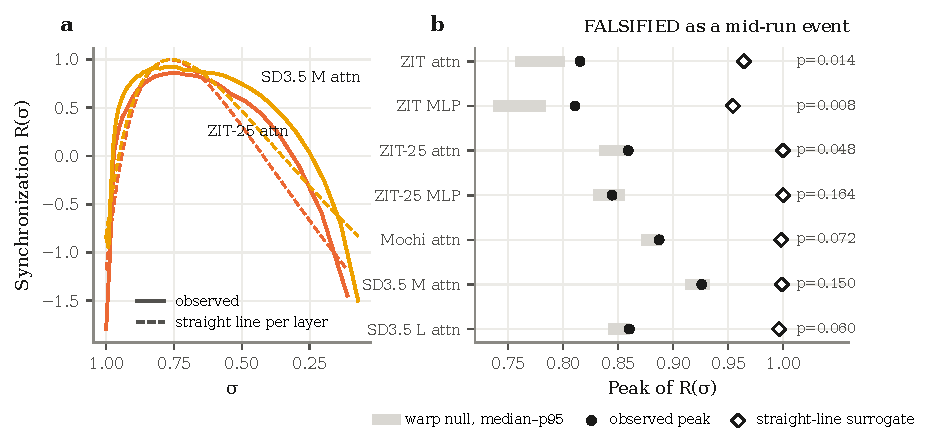
\includegraphics[width=\linewidth]{I-F12_sync_falsification}
 \caption{The historical synchronization peak is not a mid-run event. \textbf{(a)} Cross-layer order parameter $R(\sigma)$ of the population-mean field: observed against a per-layer straight-line surrogate (\TT{} and SD3.5\,M attention). The straight-line surrogate reaches a higher peak (1.00 vs 0.86; 1.00 vs 0.93). \textbf{(b)} Observed $R$ peak (0.81--0.93) against the monotone-warp null (median to p95, 500 draws) and the straight-line surrogate for seven channels: the straight-line surrogate exceeds the observed peak in 7/7; the warp null matches it ($p > 0.05$) in 4/7. The warp null is beaten only in ZIT attention and MLP ($p = 0.014$, $0.008$) and, marginally, \TT{} attention ($p = 0.048$). FALSIFIED as a mid-run synchronization event.}
 \label{fig:sync}
\end{figure}

\section{Analyzer instrument notes}\label{app:analyzer}
The layer-axis results use the CoS-PAFS Live Analyzer v3 (SHA-256 prefix \texttt{4089062551a3c900}) without modification. Four behaviours matter when it is applied to diffusion telemetry:
\begin{itemize}
 \item Its mean-profile, interval and ratio tools keep only rows with token type \texttt{generated}, so they return nothing on diffusion rows (type \texttt{step}); they were built for the language-model corpus. The layer-flow measurement on diffusion data is the dashboard's $\beta$-layer view.
 \item When a file contains both attention and MLP rows, most views average them per (layer, step) cell. Pooled Z-Image channels then show a single crossing.
 \item A header-less CSV is silently dropped by the loader. One Mochi CFG 4.5 domain file (73{,}152 rows) is affected, so Mochi CFG 4.5 results cover 9 of 10 domains; every Mochi CFG 4.5 number and figure panel in both papers inherits this coverage, and none of them enters the related--unrelated split or a lineage value. A loader for archive analysis should fail on such files instead.
 \item The Turbo archive includes four auxiliary 100-step generations, which enter step-axis views up to step 99.
\end{itemize}

\section{Estimator sensitivity}\label{app:estimators}
\begin{table}[htbp]
\centering\small
\caption{$\sigma_{50}$ and relative onset against sample size (SD3.5 Medium archive, branch-mean).}
\begin{tabular}{lcccc}
\toprule
Prompts $\times$ seeds & $n$ & $\sigma_{50}$ & Relative onset & Final $R^2$\\
\midrule
$30\times2$ & 60 & undefined (98\%) & 0.900 & 0.48\\
$60\times2$ & 120 & 0.720 & 0.867 & \\
$30\times4$ & 120 & 0.867 & 0.935 & \\
$120\times2$ & 240 & 0.843 & 0.915 & \\
$60\times4$ & 240 & 0.917 & 0.952 & \\
$120\times4$ & 480 & 0.936 & 0.956 & 0.89\\
\bottomrule
\end{tabular}
\end{table}
The fold partition alone moves $\sigma_{50}$ between $0.48$ and $0.63$ on one dataset. Simulated references for VR(4) on paths of the archive's length: random walk $0.816$--$0.828$, AR(0.8) $0.694$--$0.725$, i.i.d.\ $0.25$.

\section{Legacy instrument results}\label{app:legacy}
An early SD3.5 Medium suite (one prompt, 30 seeds per resolution, CFG 1, 100 steps, $512/768/1024$ pixels) and a CFG 1.0 versus 5.5 study at $256$ pixels were recorded with a capture path that substitutes an exponential-moving-average attention whenever it is registered. On those files depth profiles show a terminal rebound with four crossings, shape correlations of $0.989$--$0.996$ across resolutions, and a stable complex eigenpair of the local depth map. Because the instrument differs and the suite has a single prompt, these results are not used as evidence in this paper. The Round 3 captures at the same resolutions, with 60 prompts on the patched instrument, show $+,-,+,-$ rather than four crossings (\S\ref{sec:interventions}).

\section{Post hoc follow-ups on existing captures}\label{supp:posthoc}
After Round 18 was frozen, a sweep looked for analyses the existing captures allowed and the papers had not run. The checks were written down before they were run (\texttt{review/posthoc\_2026-11-10/\allowbreak PLAN.md}, SHA-256 prefix \texttt{27d056e4}, 2026-11-10 11:51 UTC) but after the data had been seen, so every result here is post hoc. The main value of the sweep is that the four Round 17 models, captured only for the tier controls, had never been used for the atlas: they are an untouched replication set for rules formed on the archive.

\begin{table}[htbp]
\centering\footnotesize
\caption{Archive rules replayed on the Round 17 models (PixArt-$\Sigma$, Cosmos-Predict2 2B: attention and MLP; SD3 Medium, SD3.5 Medium: attention; conditional branch, 60 prompts, seed 1001). Post hoc.}
\label{tab:posthocR17}
\begin{tabularx}{\linewidth}{@{}l>{\raggedright\arraybackslash}p{3.6cm}L@{}}
\toprule
Check & Rule replayed & Result\\
\midrule
RC34 & backbone (R11-5: PC1 $\ge0.70$, beats 999 depth-shift nulls) & 6 of 6 channels (PC1 $0.72$--$0.91$, rank $1.40$--$2.21$; unconditional branch 6 of 6)\\
RC35 & two components (B3, $\ge0.98$); autonomy (B4, $\Delta R^2\ge0.30$); anisotropy (B2/C1) & B3 5 of 6 (Cosmos MLP $0.967$); B4 6 of 6 ($0.51$--$0.67$); anisotropy fails in 6 of 6 (medians $0.057$--$0.114$)\\
RC36 & plateau onset in $[0.73,0.92]$ (B8) & 6 of 10 with Z1 and Z3; range $0.66$--$0.97$\\
RC37 & clock envelope signs (S4) & PixArt-$\Sigma$, Cosmos $+,+,-$ in both submodules; SD3 and SD3.5 Medium attention $+,+,+$ (all 100\% of bootstraps)\\
RC38 & layer-axis crossings & count changes with the row set in 5 of 6 channels (PixArt-$\Sigma$ MLP 4, 5 or 8): not stable\\
RC39 & first-state domain decoding & conditional branch 6 of 6 beat every baseline ($0.37$--$0.48$; scramble maximum $0.22$--$0.25$); unconditional at chance\\
RC40 & cross-model prompt geometry (S2) & unrelated attention pairs $0.04$--$0.49$ (median $0.29$), $96\%$ significant after removing text and length; PixArt-$\Sigma$$\leftrightarrow$Cosmos $0.33$--$0.44$\\
RC41 & text-to-latent handoff (R15-1) & 4 of 6; PixArt-$\Sigma$ reaches $0.5$ at step 4 of 20 instead of 2, and ends at $0.995$\\
\bottomrule
\end{tabularx}
\end{table}

\paragraph{What replicates and what narrows.} The backbone, the two-component triple, the non-autonomous depth step, first-state decoding and shared prompt geometry replicate on models that played no part in forming them. Three archive readings narrow: strong anisotropy of the uncentred second moment (it fails in all four models, so the C1 failure of the U-Net is not specific to convolution), the attention envelope $+,+,-$ (the SD3 family's conditional branch rises throughout; these captures used the card sampler rather than CoS-PAFS, Appendix~\ref{app:provenance}, which is a confound) and the plateau-onset window. The layer-axis crossing count is unstable, as RC29 found for most channels.

\paragraph{Row sets, the identity gate and decoding (RC43--RC46).} The identity gate separates Z-Image Base from Turbo through the caption rows: $0.655$ (attention) and $0.585$ (MLP) on all rows, $0.537$ and $0.904$ on caption rows, $0.945$ and $0.930$ on image rows and $0.959$ and $0.884$ centred, with split-half same weights at $0.997$ or more. On image rows the gate therefore reads the siblings in its undecided band, as it reads SD3.5 Large and Large Turbo ($0.986$, Round 18). First-state domain decoding holds on every row set of Z2 and the Round 11 Turbo session ($0.29$--$0.47$; RC45) and on the real Base ($0.54$/$0.46$; RC46).

\paragraph{The successor by depth half (RC47) and matrix regression (RC48).} SD3.5 Medium adds self-attention to its first 13 blocks (MMDiT-X). The successor tangent is $0.940$ on blocks 0--12 and $0.912$ on blocks 12--23 (same weights $0.990$ and $0.971$), so its shortfall from same weights is not concentrated in the changed blocks. A multiple regression of one model's prompt-distance matrix on another's gives the lineage pair $\beta=0.56$--$0.62$ and unrelated pairs $0.13$--$0.43$, every cell positive ($p\le0.01$), which restates the shared prompt geometry of \S\ref{sec:content}.

Three planned checks (seed estimators on the real Base, state against derivative alignment on the real lineage pair, and theme residuals for Base against Turbo) need older code ported to the new cubes and were not run.

\section{Round-8 review checks: the screen's limits}\label{supp:round8}
{\sloppy Post hoc checks RC53--RC56 (2026-11-11). The scripts are \texttt{rc53\_fpr\_inventory.py}, \texttt{rc54\_rc55\_round8.py} and \texttt{rc56\_grid12\_reconstruction.py} in the review-checks folder (\texttt{review/\allowbreak r15\_deep\_dive/\allowbreak review\_checks/}), with outputs in its \texttt{out/} folder. Summarised in \S\ref{sec:similarity} (``What the screen can and cannot claim'').\par}

\begin{table}[htbp]
\centering\scriptsize
\caption{Every depth-matched unrelated pair with an attention tangent on file (RC53). Native grid: one point per hooked layer (24 for these, so native and 24-point coincide except for PixArt-$\Sigma$$\leftrightarrow$Cosmos, 28 layers). Perm.\ p95: layer-order permutation; Surr.\ p95: smoothness-preserving surrogate (24-point grid). The ten capture pair-directions are five distinct model pairs of two types; none meets the lineage rule (p95 $+0.30$) on either grid; one lies above its permutation null on 24 points. Zero false positives among $k$ independent pairs give a one-sided 95\% upper bound of $1-0.05^{1/k}$ on the false-positive rate: $0.78$ ($k=2$), $0.45$ ($k=5$), $0.26$ ($k=10$).}
\label{tab:unrelinv}
\setlength\tabcolsep{2.5pt}
\begin{tabularx}{\linewidth}{@{}lLccccc@{}}
\toprule
Captures & Model pair & 24-pt & Perm. & Surr. & Native & Perm. (nat.)\\
\midrule
PixArt-$\Sigma$$\leftrightarrow$Cosmos 2B & PixArt-$\Sigma$ / Cosmos-Predict2 2B & 0.30 & 0.26 & 0.24 & 0.20 & 0.26\\
ACE turbo 6$\leftrightarrow$SD3.5 M (R17) & ACE-Step turbo / SD3.5 Medium & $-$0.07 & 0.32 & 0.26 & $-$0.07 & 0.35\\
ACE turbo 6$\leftrightarrow$SD3 M & ACE-Step turbo / SD3 Medium & $-$0.05 & 0.31 & 0.29 & $-$0.05 & 0.34\\
ACE turbo 6$\leftrightarrow$SD3.5 M (R11) & ACE-Step turbo / SD3.5 Medium & $-$0.09 & 0.33 & 0.26 & $-$0.09 & 0.36\\
ACE Base$\leftrightarrow$SD3.5 M (R17) & ACE-Step Base / SD3.5 Medium & $-$0.10 & 0.29 & 0.26 & $-$0.10 & 0.33\\
ACE Base$\leftrightarrow$SD3 M & ACE-Step Base / SD3 Medium & $-$0.06 & 0.30 & 0.34 & $-$0.06 & 0.33\\
ACE Base$\leftrightarrow$SD3.5 M (R11) & ACE-Step Base / SD3.5 Medium & $-$0.11 & 0.30 & 0.27 & $-$0.11 & 0.34\\
ACE turbo 8$\leftrightarrow$SD3.5 M (R17) & ACE-Step turbo / SD3.5 Medium & $-$0.16 & 0.34 & 0.29 & $-$0.16 & 0.37\\
ACE turbo 8$\leftrightarrow$SD3 M & ACE-Step turbo / SD3 Medium & $-$0.15 & 0.34 & 0.34 & $-$0.15 & 0.38\\
ACE turbo 8$\leftrightarrow$SD3.5 M (R11) & ACE-Step turbo / SD3.5 Medium & $-$0.17 & 0.36 & 0.30 & $-$0.17 & 0.37\\
\bottomrule
\end{tabularx}
\end{table}

\begin{table}[htbp]
\centering\scriptsize\setlength\tabcolsep{2pt}
\caption{The tangent by depth frequency (RC54, native grid $n$). Each state's depth differences are expanded in an orthonormal DCT-II basis along depth; the cosine is recomputed on the low ($k<(n-1)/4$), middle and high ($k\ge(n-1)/2$) coefficients and on the lowest 11, the most a 12-point grid can hold. Band permutation-null p95 in parentheses (300 draws). Upper energy: share of the first model's difference energy in the high band. The full-band cosine equals the native tangent.}
\label{tab:bands}
\begin{tabularx}{\linewidth}{@{}>{\raggedright\arraybackslash}p{1.9cm}Lcccccccc@{}}
\toprule
Relation & Pair & Sub & $n$ & Native & Low & Middle & High & 12-pt & Upper $E$\\
\midrule
same weights, sessions & Z3$\leftrightarrow$ZIT & attn & 30 & 0.99 & 0.98 (0.35) & 0.99 (0.45) & 0.99 (0.31) & 0.99 (0.42) & 0.66\\
same weights, sessions & Z3$\leftrightarrow$ZIT & mlp & 30 & 0.99 & 0.99 (0.36) & 0.99 (0.36) & 0.99 (0.29) & 0.99 (0.30) & 0.70\\
same weights, sessions & SD3.5 M (R17)$\leftrightarrow$SD3.5 M (R11) & attn & 24 & 0.98 & 0.99 (0.70) & 0.98 (0.44) & 0.97 (0.31) & 0.99 (0.50) & 0.41\\
same weights, sessions & ACE turbo 8$\leftrightarrow$ACE turbo 6 & attn & 24 & 0.92 & 0.83 (0.55) & 0.89 (0.48) & 0.92 (0.39) & 0.88 (0.46) & 0.89\\
same weights, sessions & SD3.5 L (R18)$\leftrightarrow$SD3.5 L (archive) & attn & 38 & 1.00 & 1.00 (0.49) & 0.99 (0.45) & 1.00 (0.38) & 1.00 (0.44) & 0.90\\
same weights, run & PixArt-$\Sigma$$\leftrightarrow$PixArt-$\Sigma$ uncond & attn & 28 & 1.00 & 0.99 (0.40) & 1.00 (0.43) & 1.00 (0.27) & 0.99 (0.35) & 0.67\\
successor & SD3 M$\leftrightarrow$SD3.5 M (R17) & attn & 24 & 0.93 & 0.96 (0.68) & 0.90 (0.42) & 0.91 (0.35) & 0.94 (0.48) & 0.46\\
distillation, documented & SD3.5 L (R18)$\leftrightarrow$SD3.5 L Turbo & attn & 38 & 0.90 & 0.94 (0.45) & 0.74 (0.44) & 0.91 (0.38) & 0.91 (0.43) & 0.90\\
distillation & ACE Base$\leftrightarrow$ACE turbo 8 & attn & 24 & 0.79 & 0.67 (0.55) & 0.72 (0.45) & 0.81 (0.34) & 0.65 (0.36) & 0.91\\
distillation & ACE Base$\leftrightarrow$ACE turbo 8 & mlp & 24 & 0.59 & 0.73 (0.53) & 0.74 (0.46) & 0.46 (0.23) & 0.74 (0.46) & 0.55\\
sibling & Z1 (Base)$\leftrightarrow$ZIT & attn & 30 & 0.55 & 0.65 (0.65) & 0.78 (0.51) & 0.46 (0.33) & 0.67 (0.52) & 0.65\\
sibling & Z1 (Base)$\leftrightarrow$ZIT & mlp & 30 & 0.77 & 0.82 (0.38) & 0.59 (0.34) & 0.80 (0.29) & 0.78 (0.27) & 0.67\\
unrelated & PixArt-$\Sigma$$\leftrightarrow$Cosmos 2B & attn & 28 & 0.20 & 0.66 (0.54) & 0.36 (0.49) & 0.01 (0.34) & 0.56 (0.41) & 0.67\\
unrelated & PixArt-$\Sigma$$\leftrightarrow$Cosmos 2B & mlp & 28 & 0.57 & 0.90 (0.47) & 0.41 (0.33) & 0.28 (0.24) & 0.78 (0.32) & 0.21\\
unrelated, cross-modal & ACE Base$\leftrightarrow$SD3.5 M (R17) & attn & 24 & $-$0.10 & 0.58 (0.50) & $-$0.22 (0.43) & $-$0.25 (0.39) & 0.35 (0.39) & 0.91\\
unrelated, cross-modal & ACE turbo 8$\leftrightarrow$SD3 M & attn & 24 & $-$0.15 & 0.36 (0.51) & $-$0.20 (0.49) & $-$0.25 (0.45) & 0.17 (0.41) & 0.89\\
unrelated, cross-modal & ACE turbo 6$\leftrightarrow$SD3.5 M (R11) & attn & 24 & $-$0.09 & 0.46 (0.52) & $-$0.25 (0.48) & $-$0.18 (0.37) & 0.18 (0.42) & 0.89\\
\bottomrule
\end{tabularx}
\end{table}

\begin{table}[htbp]
\centering\scriptsize
\caption{MLP tangent variants on the pairs with row-split captures (RC55, native grid, 300-draw nulls). Image rows equal all rows for PixArt-$\Sigma$ and Cosmos, whose hooks read image tokens only. End trim: first and last hooked layer removed.}
\label{tab:mlpvar}
\begin{tabularx}{\linewidth}{@{}Llllcccc@{}}
\toprule
Relation & Pair & Statistic & End trim & $n$ & Tangent & Perm.\ p95 & Surr.\ p95\\
\midrule
sibling & Z2 (Base)$\leftrightarrow$Turbo R11 & all & no & 30 & 0.77 & 0.21 & 0.37\\
sibling & Z2 (Base)$\leftrightarrow$Turbo R11 & all & yes & 28 & 0.79 & 0.22 & 0.39\\
sibling & Z2 (Base)$\leftrightarrow$Turbo R11 & image & no & 30 & 0.74 & 0.21 & 0.33\\
sibling & Z2 (Base)$\leftrightarrow$Turbo R11 & image & yes & 28 & 0.80 & 0.22 & 0.35\\
sibling & Z2 (Base)$\leftrightarrow$Turbo R11 & centred & no & 30 & 0.52 & 0.17 & 0.25\\
sibling & Z2 (Base)$\leftrightarrow$Turbo R11 & centred & yes & 28 & 0.50 & 0.15 & 0.22\\
sibling & Z2 (Base)$\leftrightarrow$Turbo R11 & top8 removed & no & 30 & 0.51 & 0.20 & 0.27\\
sibling & Z2 (Base)$\leftrightarrow$Turbo R11 & top8 removed & yes & 28 & 0.70 & 0.24 & 0.34\\
unrelated & PixArt-$\Sigma$$\leftrightarrow$Cosmos 2B & all & no & 28 & 0.57 & 0.17 & 0.29\\
unrelated & PixArt-$\Sigma$$\leftrightarrow$Cosmos 2B & all & yes & 26 & 0.39 & 0.21 & 0.23\\
unrelated & PixArt-$\Sigma$$\leftrightarrow$Cosmos 2B & image & no & 28 & 0.57 & 0.17 & 0.29\\
unrelated & PixArt-$\Sigma$$\leftrightarrow$Cosmos 2B & image & yes & 26 & 0.39 & 0.21 & 0.23\\
unrelated & PixArt-$\Sigma$$\leftrightarrow$Cosmos 2B & centred & no & 28 & 0.27 & 0.21 & 0.21\\
unrelated & PixArt-$\Sigma$$\leftrightarrow$Cosmos 2B & centred & yes & 26 & 0.26 & 0.18 & 0.16\\
unrelated & PixArt-$\Sigma$$\leftrightarrow$Cosmos 2B & top8 removed & no & 28 & 0.76 & 0.15 & 0.31\\
unrelated & PixArt-$\Sigma$$\leftrightarrow$Cosmos 2B & top8 removed & yes & 26 & 0.55 & 0.21 & 0.26\\
same weights, run & PixArt-$\Sigma$$\leftrightarrow$PixArt-$\Sigma$ uncond & all & no & 28 & 1.00 & 0.22 & 0.39\\
same weights, run & PixArt-$\Sigma$$\leftrightarrow$PixArt-$\Sigma$ uncond & all & yes & 26 & 1.00 & 0.23 & 0.37\\
same weights, run & PixArt-$\Sigma$$\leftrightarrow$PixArt-$\Sigma$ uncond & image & no & 28 & 1.00 & 0.22 & 0.39\\
same weights, run & PixArt-$\Sigma$$\leftrightarrow$PixArt-$\Sigma$ uncond & image & yes & 26 & 1.00 & 0.23 & 0.37\\
same weights, run & PixArt-$\Sigma$$\leftrightarrow$PixArt-$\Sigma$ uncond & centred & no & 28 & 0.99 & 0.19 & 0.32\\
same weights, run & PixArt-$\Sigma$$\leftrightarrow$PixArt-$\Sigma$ uncond & centred & yes & 26 & 0.94 & 0.15 & 0.34\\
same weights, run & PixArt-$\Sigma$$\leftrightarrow$PixArt-$\Sigma$ uncond & top8 removed & no & 28 & 1.00 & 0.17 & 0.35\\
same weights, run & PixArt-$\Sigma$$\leftrightarrow$PixArt-$\Sigma$ uncond & top8 removed & yes & 26 & 1.00 & 0.23 & 0.36\\
\bottomrule
\end{tabularx}
\end{table}

\begin{table}[htbp]
\centering\scriptsize\setlength\tabcolsep{2pt}
\caption{Reconstruction of the 12-point tangent from native-grid depth frequencies (RC56). 12-pt: the tangent after linear interpolation of the native profile onto 12 points. Ideal LP: the same after removing, before interpolation, every depth-cosine component of the profile that 12 points cannot represent ($k\ge11$). Band: the RC54 12-point band of the native differences (Table~\ref{tab:bands}). Folded: percentage of the 12-point difference energy contributed by the removed components, which linear interpolation folds back into the represented ones. An ideal low-pass filter would give 12-pt = Ideal LP and Folded = 0.}
\label{tab:recon12}
\begin{tabularx}{\linewidth}{@{}>{\raggedright\arraybackslash}p{1.9cm}Lccccccc@{}}
\toprule
Relation & Pair & Sub & $n$ & Native & 12-pt & Ideal LP & Band & Folded (\%)\\
\midrule
same weights, sessions & Z3$\leftrightarrow$ZIT & attn & 30 & 0.99 & 0.99 & 0.98 & 0.99 & 35\\
same weights, sessions & Z3$\leftrightarrow$ZIT & mlp & 30 & 0.99 & 0.99 & 0.99 & 0.99 & 21\\
same weights, sessions & SD3.5 M (R17)$\leftrightarrow$SD3.5 M (R11) & attn & 24 & 0.98 & 0.98 & 0.99 & 0.99 & 8\\
same weights, sessions & ACE turbo 8$\leftrightarrow$ACE turbo 6 & attn & 24 & 0.92 & 0.90 & 0.87 & 0.88 & 33\\
same weights, sessions & SD3.5 L (R18)$\leftrightarrow$SD3.5 L (archive) & attn & 38 & 1.00 & 0.99 & 1.00 & 1.00 & 27\\
same weights, run & PixArt-$\Sigma$$\leftrightarrow$PixArt-$\Sigma$ uncond & attn & 28 & 1.00 & 0.99 & 0.99 & 0.99 & 28\\
successor & SD3 M$\leftrightarrow$SD3.5 M (R17) & attn & 24 & 0.93 & 0.93 & 0.96 & 0.94 & 10\\
distillation, documented & SD3.5 L (R18)$\leftrightarrow$SD3.5 L Turbo & attn & 38 & 0.90 & 0.96 & 0.97 & 0.91 & 27\\
distillation & ACE Base$\leftrightarrow$ACE turbo 8 & attn & 24 & 0.79 & 0.51 & 0.67 & 0.65 & 23\\
distillation & ACE Base$\leftrightarrow$ACE turbo 8 & mlp & 24 & 0.59 & 0.59 & 0.53 & 0.74 & 14\\
sibling & Z1 (Base)$\leftrightarrow$ZIT & attn & 30 & 0.55 & 0.70 & 0.66 & 0.67 & 16\\
sibling & Z1 (Base)$\leftrightarrow$ZIT & mlp & 30 & 0.77 & 0.81 & 0.84 & 0.78 & 20\\
unrelated & PixArt-$\Sigma$$\leftrightarrow$Cosmos 2B & attn & 28 & 0.20 & 0.60 & 0.65 & 0.56 & 28\\
unrelated & PixArt-$\Sigma$$\leftrightarrow$Cosmos 2B & mlp & 28 & 0.57 & 0.80 & 0.79 & 0.78 & 6\\
unrelated, cross-modal & ACE Base$\leftrightarrow$SD3.5 M (R17) & attn & 24 & $-$0.10 & 0.56 & 0.57 & 0.35 & 23\\
unrelated, cross-modal & ACE turbo 8$\leftrightarrow$SD3 M & attn & 24 & $-$0.15 & 0.62 & 0.53 & 0.17 & 33\\
unrelated, cross-modal & ACE turbo 6$\leftrightarrow$SD3.5 M (R11) & attn & 24 & $-$0.09 & 0.56 & 0.49 & 0.18 & 35\\
\bottomrule
\end{tabularx}
\end{table}

\section{Capture cost}\label{supp:cost}
Per hook and sampling step the capture node forms the $D\times D$ Gram matrix $X^\top X/N$ in single precision and takes its symmetric eigendecomposition (\texttt{torch.linalg.eigvalsh}), a cost of order $ND^2+D^3$ on the GPU, and stores three numbers plus metadata, so storage grows with layers $\times$ steps $\times$ generations, not with $N$ or $D$. The full passive archive (six diffusion campaigns and the language-model controls) is about 0.7\,GB of CSV. Wall-clock overhead was not benchmarked systematically; for the largest image model here (SD3.5 Large, $D=2432$, 38 layers, 28 steps, one hook) it is one eigendecomposition of a $2432\times2432$ matrix per layer and step. Routine auditing would only need the first sampling state (the identity gate) or a few states, which is a small fraction of a full capture. A benchmark of overhead against model size and resolution is a Mode-III item.

\section{Supplementary figures}\label{app:supp}
\begin{figure}[h]
 \centering
 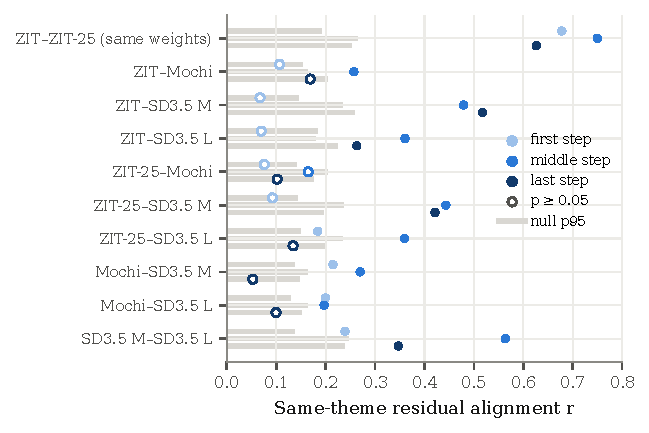
\includegraphics[width=\linewidth]{I-S1_theme_residual}
 \caption{Same-theme residual alignment after each model/time backbone is removed, for all model pairs at the first, middle and last step. Bars show the theme-label permutation null p95. The two Turbo campaigns (same weights): 0.63--0.75 at every step, the strongest; at the first step every other pair is $\le 0.24$; by the middle step unrelated pairs reach up to 0.48, and up to 0.52 by the last step (ZIT$\leftrightarrow$SD3.5\,M). Theme alignment is strongest for the same weights at every step and specific to them only at the first step.}
 \label{fig:S1}
\end{figure}

\begin{figure}[h]
 \centering
 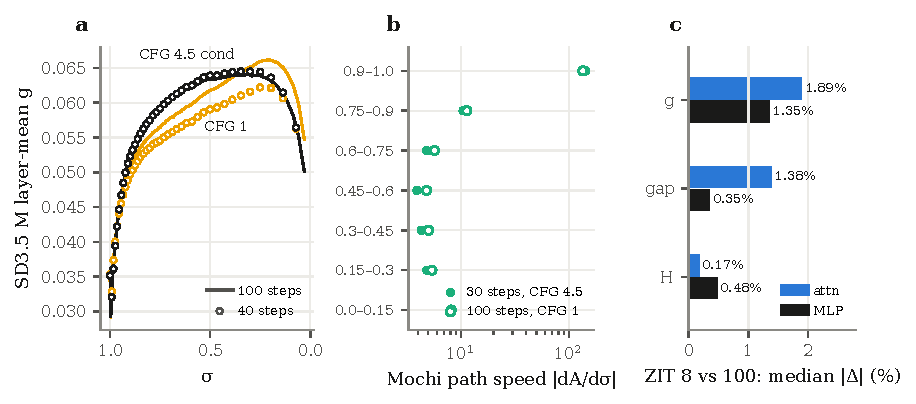
\includegraphics[width=\linewidth]{I-S2_stepcount_controls}
 \caption{Per-$\sigma$ geometry changes by at most 2--3\% between 8/40 and 100 steps. \textbf{(a)} SD3.5\,M, one prompt, explicit cond branch: layer-mean attention $g(\sigma)$ at 40 (markers) and 100 steps (lines), CFG\,1 and CFG\,4.5. The same-prompt 40$\to$100 shift is 0.033 at CFG\,1 (seed-split null p95 0.027, $p = 0.023$) and 0.007 at CFG\,4.5 (p95 0.022, $p = 0.70$). \textbf{(b)} Mochi 30 vs 100 steps: path speed by $\sigma$ band (ratio 0.81--1.06). The two arms also differ in CFG (4.5 vs 1). \textbf{(c)} ZIT 8 vs 100 steps at matched $\sigma$: median relative difference of $g$ (1.9\% attn / 1.4\% MLP), gap (1.4\% / 0.4\%) and $H$ (0.2\% / 0.5\%). The 100-step set contains only 4 generations.}
 \label{fig:S2}
\end{figure}

\begin{figure}[h]
 \centering
 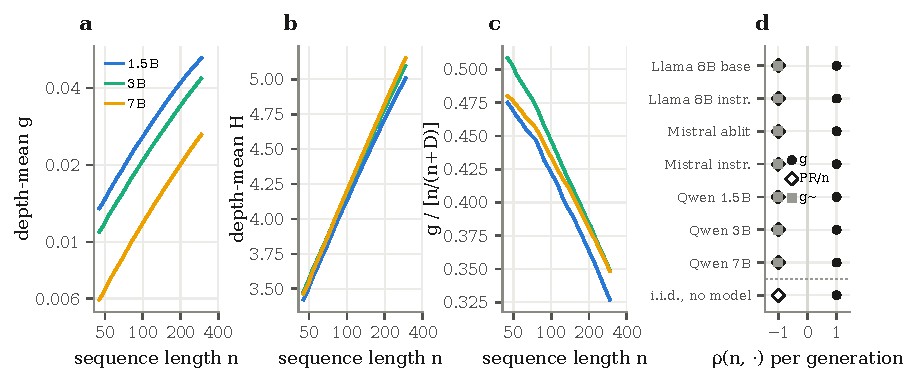
\includegraphics[width=\linewidth]{I-S3_qwen_context_clock}
 \caption{Why per-token phase claims for autoregressive models are not made. The v1 LLM capture re-encodes the full context at every token without a KV cache, so each logged value is a running statistic of a nested $n\times D$ matrix. \textbf{(a, b)} Depth-mean $g$ and $H$ of generated tokens against sequence length $n$ for Qwen2.5 1.5B/3B/7B (median per $n$ bin). \textbf{(c)} $g$ normalized by the finite-sample baseline $n/(n+D)$ remains monotone in $n$. \textbf{(d)} Median within-generation Spearman $\rho(n,\cdot)$ for all seven LLM captures: $\rho = 1.00$ for $g$ and $\le -0.999$ for PR$/n$ and $\tilde g$. The bottom row is a model-free reference (Round 9, preregistered): nested running statistics of i.i.d.\ Gaussian rows (180 simulations; isotropic, power-law and spiked spectra; $D=1536$ and $4096$) give the same $\rho$ without any network, so the monotonicity is a property of the capture. The Qwen multiscale $\beta$ "anomaly" therefore is a context-length clock, and it is demoted.}
 \label{fig:S3}
\end{figure}

\begin{figure}[h]
 \centering
 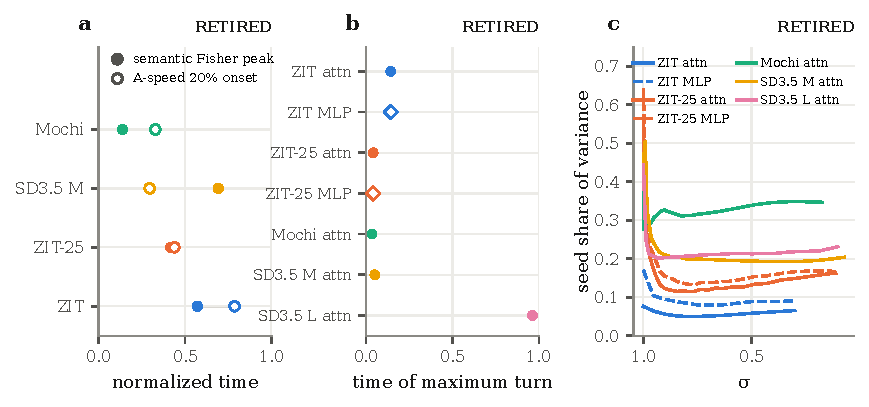
\includegraphics[width=\linewidth]{I-S4_negative_atlas}
 \caption{Retired claims. Every panel is marked RETIRED. \textbf{(a)} "The semantic decoder maximum is the universal C1 time": the smoothed semantic Fisher peak (0.14--0.69) does not track the A-speed 20\% onset (0.30--0.79) in normalized time (differences $-0.21$ to $+0.40$). \textbf{(b)} "Trajectory curvature gives a universal C1 detector": the time of the maximum turning angle falls in the early transient ($\tau \le 0.14$) in six of seven channels and at $\tau = 0.96$ in SD3.5\,L. \textbf{(c)} "Universal seed collapse": seed share of within-step variance along $\sigma$ (ANOVA). It ranges from 0.05--0.08 (ZIT attention) to a peak of 0.64 (25-step Turbo MLP, \TT{}), with no common collapse. The retired passive-susceptibility peak is not shown, because no per-channel values are stored.}
 \label{fig:S4}
\end{figure}

\begin{figure}[h]
 \centering
 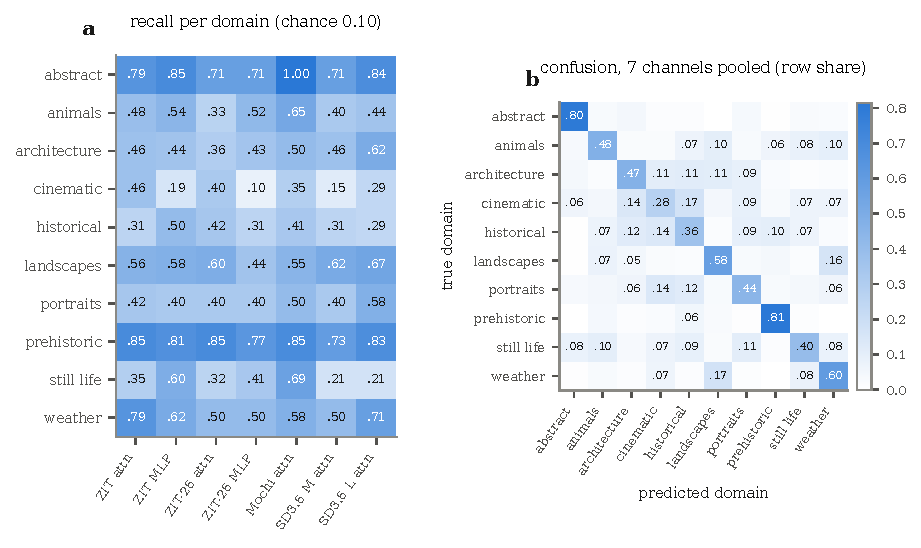
\includegraphics[width=\linewidth]{I-S5_domain_confusion}
 \caption{Which domains the first-state decoder recovers (descriptive). Same decoder, features and prompt-grouped folds as Fig.~\ref{fig:decode}a, with out-of-fold predictions. \textbf{(a)} Recall per domain for the seven archive channels (chance 0.10). Every cell is above chance except cinematic prompts in 25-step Turbo MLP (\TT{}; 0.10). Abstract (0.71--1.00) and prehistoric (0.73--0.85) prompts are recovered best, cinematic (0.10--0.46) and still-life prompts (0.21--0.69) worst. \textbf{(b)} Confusion matrix summed over the seven channels, as row shares; values below 0.05 are not printed. Errors spread over several domains rather than concentrating in one pair; the largest off-diagonal shares are landscapes$\leftrightarrow$weather (0.16, 0.17).}
 \label{fig:S5}
\end{figure}


\end{document}
